\documentclass[12pt]{jarticle}
\usepackage[utf8]{inputenc}
\usepackage[top=30truemm, bottom=30truemm, left=20truemm, right=20truemm]{geometry}
\usepackage{amsmath}
\usepackage{amssymb}
\usepackage{mathtools}
\usepackage{siunitx}
\usepackage{bm}
\usepackage[dvipdfmx]{graphicx}
\usepackage[dvipdfmx]{color}
\usepackage[subrefformat=parens]{subcaption}
\usepackage{booktabs}
\usepackage{tabularx}
\usepackage{tocloft}
\usepackage{enumerate}
\usepackage{url}
\usepackage{multirow}
\usepackage{caption}
\usepackage{enumitem}
\usepackage{makecell}
\usepackage{array}
\usepackage{algorithm}
\usepackage{algpseudocode}
\usepackage{physics}
\usepackage{hyperref}

\numberwithin{equation}{section}    % 数式番号にセクション番号をつける
\numberwithin{figure}{section}      % 図番号にセクション
\numberwithin{table}{section}      % 図番号にセクション

% \renewcommand{\figurename}{Fig.}    % 図 -> Fig.
% \renewcommand{\tablename}{Table }   % 表 -> Table

\renewcommand{\baselinestretch}{1.1}

\newlength{\figcaptionskip}
\setlength{\figcaptionskip}{5pt} % 図のキャプション間隔
\newlength{\tabcaptionskip}
\setlength{\tabcaptionskip}{-5pt} % 表のキャプション間隔
\captionsetup[figure]{skip=\figcaptionskip}
\captionsetup[table]{skip=\tabcaptionskip}

\setlist[enumerate]{topsep=5pt, partopsep=5pt, itemsep=0pt, parsep=0pt}
\setlength{\topsep}{5pt}
\setlength{\partopsep}{5pt}

% data
\newcommand{\dataset}{\mathcal{D}}
\newcommand{\dimLower}{d}
\newcommand{\dimUpper}{D}
\newcommand{\heightLower}{h}
\newcommand{\heightUpper}{H}
\newcommand{\indexLower}{i}
\newcommand{\indexUpper}{I}
\newcommand{\inputLower}{x}
\newcommand{\inputUpper}{X}
\newcommand{\numLower}{n}
\newcommand{\numUpper}{N}
\newcommand{\outputLower}{y}
\newcommand{\outputUpper}{Y}
\newcommand{\timeLower}{t}
\newcommand{\timeUpper}{T}
\newcommand{\widthLower}{w}
\newcommand{\widthUpper}{W}

% model
\newcommand{\biasLower}{b}
\newcommand{\classLower}{c}
\newcommand{\classUpper}{C}
\newcommand{\dilationUpper}{R}
\newcommand{\numHeadLower}{h}
\newcommand{\numHeadUpper}{H}
\newcommand{\kernelSizeLower}{k}
\newcommand{\kernelSizeUpper}{K}
\newcommand{\modelLower}{f}
\newcommand{\modelUpper}{F}
\newcommand{\strideUpper}{S}
\newcommand{\weightLower}{w}
\newcommand{\weightUpper}{W}
\newcommand{\weightAndBias}{\theta}

% other
\newcommand{\binaryMaskLower}{m}
\newcommand{\binaryMaskUpper}{M}
\newcommand{\optimEmaConst}{\beta}
\newcommand{\epochLower}{e}
\newcommand{\counter}{\tau}
\newcommand{\learningRate}{\eta}
\newcommand{\lossFuncUpper}{L}
\newcommand{\normScale}{\gamma}
\newcommand{\normShift}{\beta}
\newcommand{\probaLower}{p}
\newcommand{\regConst}{\lambda}

% math
\newcommand{\closedinterval}[2]{[#1, #2]}
\newcommand{\openinterval}[2]{(#1, #2)}
\newcommand{\leftclosedinterval}[2]{[#1, #2)}
\newcommand{\rightclosedinterval}[2]{(#1, #2]}
\newcommand{\realSet}{\mathbb{R}}
\newcommand{\naturalSet}{\mathbb{N}}

% operator
\newcommand{\elemMul}{\odot}
\newcommand{\elemSum}{\oplus}

\allowdisplaybreaks[4]

\begin{document}

\begin{titlepage}
    \begin{center}
        {\Large 2024年度後期 修士論文}
        \vspace{120truept}

        {\huge 深層学習による口唇音声変換に関する研究}
        \vspace{30truept}

        {\huge A Study on the Conversion from Lip-Video to Speech Using a Deep Learning Technique}
        \vspace{120truept}

        {\Large 2025年月日}
        \vspace{10truept}

        {\Large 九州大学芸術工学府音響設計コース}
        \vspace{70truept}

        {\Large 2DS23095M}
        \vspace{10truept}

        {\Large 南 汰翼}
        \vspace{10truept}

        {\Large MINAMI Taisuke}
        \vspace{30truept}

        {\Large 研究指導教員 鏑木 時彦 教授}
    \end{center}
\end{titlepage}

\section*{概要}
\thispagestyle{empty}
\clearpage

\setcounter{tocdepth}{3}
\tableofcontents
\thispagestyle{empty}
\clearpage

\pagestyle{plain}
\setcounter{page}{1}

\section{序論}
\subsection{背景}
音声は基本的なコミュニケーション手段として,人々の日常生活において重要な役割を果たしている.しかし,癌などの病気で喉頭を摘出すると,声帯振動による音声生成が不可能になり,従来の発声手段を失う.このような場合の代用音声手法として,電気式人工喉頭や食道発声,シャント発声があるが,自然で聞き取りやすい音声を生成することが難しかったり,習得に訓練を必要としたり,器具の交換のための定期的な手術を必要とするといった課題がある.これに対して本研究では,新たな代用音声手法として,深層学習を活用して口唇の動きと音声波形の関係性を学習することで,口唇の動きから音声を合成するアプローチを提案する.この手法により,訓練や手術を必要とせずとも,自然な声でのコミュニケーションを可能にすることを目指す.

% 音声は基本的なコミュニケーションの手段であり,人と人とのコミュニケーションの場面において,重要な役割を果たしている.音声は,肺からの呼気流による声帯の振動が音源波を生成し,声道特性に伴ったフィルタリングと口唇からの放射特性に従って生成される.これより,音声の生成には音源を作り出す声帯やその制御のための喉頭,舌や口唇といった調音器官の働きが重要となる.しかし,癌などの重い病気で喉頭を摘出した場合,音源波を生成することができなくなるため,これまで通り発声を行うことが不可能になってしまう.このようなコミュニケーション機能の喪失に対し,現在でも電気式人工喉頭や食道発声,シャント発声といった代用音声手法が存在する.電気式人工喉頭では,専用の発振器を顎下に当てて振動を加えることにより,それを音源とした発声を行う.発振器を用意すれば容易に発声することが可能であるが,生成される音声のピッチが発振器の振動に依存してしまうため,抑揚のない単調な音声になってしまう.食道発声では,まず口や鼻から食道内に空気を取り込み,その空気を逆流させることで食道入口部の粘膜を振動させることによって発声する.電気式人工喉頭と違って道具を必要とせず,ピッチも本人が調節できるが,その習得に長期間の訓練を要する.シャント発声では,手術によって気管と食道を繋ぐ管を設ける.これにより,息を吐き出す際に設けられた喉の穴を手で塞ぐことによって肺からの呼気流が食道に流れる.そのため,食道発声と同様に粘膜の振動を音源とし,発声することが可能となる.習得は容易であり,比較的自然に話すことが可能となるが,設けられた管を交換するための定期的な手術が必要となる.このように,現在用いられている代用音声手法にはそれぞれデメリットが存在する.

% これに対し,本研究ではビデオカメラで撮影した口唇の動きから音声合成を行うことによる,新たな代用音声手法を検討する.本来,音声は声帯の振動や声道の形状に依存して生成されるものであり,口唇の動きのみから音声波形を直接推定することは困難である.そこで,近年画像や自然言語処理,音声といった分野において成果を上げている深層学習を活用し,口唇の動きと音声の間の関係を学習することで推定を行う.これにより,従来の代用音声手法よりも自然性の高い音声を,訓練や定期的な手術の必要なく提供することを目指す.

% これまでの動画音声合成は英語が中心に検討が進んでおり,近年ではYouTube上のデータを収集,処理することによって構築した大規模データセット\cite{afouras2018lrs3,chung2018voxceleb2}を用いることで,大規模で表現力の高いモデルが構築可能となっている.特に,従来行われてきた教師あり学習のみならず,動画と音声の関係性を自己教師あり学習(Self Supervised Learning; SSL)によって学習し,そのモデルを動画音声合成や,動画からテキストを推定するVisual Speech Recognition(VSR)にFineTuningするアプローチが提案され,その有効性が示されている.自己教師あり学習モデルにもいくつかの種類があり,近年多くの研究で応用例のあるAVHuBERT\cite{shi2022learning}は,動画・音声の入力領域においてマスクされた区間の予測と,予測対象の更新を繰り返して学習を進めていくモデルである.予測対象の更新は5回行われ,1回目は音声波形から計算されるMFCCをクラスタリングした結果を利用するが,2回目以降はモデルの中間特徴量をクラスタリングした結果を新たな予測対象に設定する.更新のたびに再度モデルをランダム初期化して再学習するが,その予測対象の複雑さが増していくことによって,学習が促進されるようなメカニズムとなっている.また,これに類似したVATLM\cite{zhu2023vatlm}は,動画と音声のみならずテキストも加えた学習によって,精度改善を達成した.その他,StudentとTeacherという二つのネットワークを利用し,Teacherから出力される特徴量をStudentがマスクされた入力から予測することによって学習を進めるRAVEn\cite{haliassos2022jointly}やAV-data2vec\cite{lian2023av},RAVEnの改善版として提案されたBRAVEn\cite{haliassos2024braven}など,多くのモデルが提案されている.

近年の動画音声合成では,LRS3\cite{afouras2018lrs3}やVoxCeleb2\cite{chung2018voxceleb2}などの大規模データセットを活用して構築された,自己教師あり学習(Self Supervised Learning; SSL)モデルをFineTuningすることの有効性が示されている.特に,近年の動画音声合成においてはAVHuBERT\cite{shi2022learning}というモデルが動画からの特徴抽出器として採用される場合が多い.AVHuBERTは,動画と音声の対応関係をMasked Predictionという自己教師あり学習方法により捉えたモデルであり,Modality Dropoutという工夫により,自己教師あり学習時には動画と音声の両方を入力とするものの,FineTuning時には動画あるいは音声のみを入力とできる柔軟性を持ち合わせている.これに加え,従来の動画音声においては動画からの予測対象としてメルスペクトログラムが選択されることが多かったが,近年ではこれにテキストや,音声SSLモデルであるHuBERTを利用して得られた離散特徴量を合わせて予測対象とする,マルチタスク学習の有効性が示されている\cite{kim2023lip_multitask,choi2023intelligible}.

% 近年の動画音声合成では,こういったSSLモデルを動画からの特徴抽出器として活用しつつ,さらなる工夫によって精度改善を達成している.動画音声合成について,\cite{kim2023lip_multitask}では予測対象として従来用いられてきたメルスペクトログラムに加え,テキストを予測するマルチタスク学習手法を提案した.損失においては上記の二つに加え,予測したメルスペクトログラムを事前学習済みの音声認識モデルに入力して得られる特徴表現も採用した.音声波形はメルスペクトログラムに対してGriffin-Limアルゴリズムを適用することで獲得しており,従来のメルスペクトログラムのみを損失とする手法に対して客観評価指標における改善を達成した.これに続き,\cite{choi2023intelligible}では前述した手法がテキストアノテーションされたデータのみにしか用いることができないという課題を解消するため,テキストと同様に言語的な情報を持つと考えられている,音声SSLモデルのHuBERT\cite{hsu2021hubert}を利用して得られるHuBERT離散特徴量を用いる手法を提案した.ここで,HuBERT離散特徴量は,HuBERTのTransformer層出力に対してk-means法によるクラスタリングを適用することで得られる.また,予測されたメルスペクトログラムとHuBERT離散特徴量の両方を入力とするMulti-input Vocoderと,Multi-input Vocoderの学習時にメルスペクトログラムにノイズをかけるデータ拡張手法を合わせて提案し,客観評価と主観評価の両方で\cite{kim2023lip_multitask}を含む既存手法に対する改善を達成した.加えて,ここではAVHuBERTの転移学習についても合わせて検討が行われ,これによってさらに性能を改善できることを示した.手法\cite{choi2023intelligible}に関連して,上記のようなマルチタスク学習手法以外にも,HuBERT離散特徴量や,離散化する前の連続特徴量を音声波形までの中間特徴量として扱う手法が存在する.例えば,\cite{hsu2023revise}ではメルスペクトログラムの推定を行わず,HuBERT離散特徴量のみを推定して音声波形に変換する手法が提案された.\cite{choi2023intelligible}では離散化におけるクラスタ数を200としていたのに対して,\cite{hsu2023revise}ではクラスタ数を2000と大きく取っている点で実装が異なっている.メルスペクトログラムを省略する分,クラスタリングによる情報圧縮の程度を軽減することで,音声波形への変換に十分な情報を保持する目的があると考えられる.また,\cite{choi2023intelligible}や\cite{hsu2023revise}ではAVHuBERTを直接動画音声合成にFineTuningしていた一方で,\cite{sahipjohn2023robustl2s}ではAVHuBERTをVSRによってFineTuningし,その後重みを固定した上で特徴抽出器として利用するアプローチを提案している.この手法では,VSRでFineTuningされたAVHuBERTから得られる動画特徴量を入力とし,HuBERT特徴量を予測するネットワークが追加で学習され,HuBERT特徴量のみから音声波形に変換するボコーダを用いることで動画音声合成が実現された.ここで,HuBERT特徴量と表した予測対象について,この研究では他の研究においても検討されたHuBERT離散特徴量だけでなく,クラスタリングによって離散化する前の連続値を用いる場合,離散値と連続値の両方を予測対象とする場合が検討され,連続値のみを予測対象とした場合が最も客観評価指標が優れていたことが示されている.検討された離散値のクラスタ数が100であったことと,\cite{hsu2023revise}の検討とを合わせると,HuBERT離散特徴量のみを用いて音声波形に変換するアプローチを取るのであれば,クラスタ数を十分大きく取る必要があることが示唆される.

% 一方VSRについて,\cite{yeo2024akvsr}では,HuBERT離散特徴量から純粋な言語情報のみを持つCompact Audio Memoryを構築し,これを動画特徴量とアテンションで関連付ける手法を提案した.ここで,Compact Audio MemoryはHuBERT離散特徴量,すなわちインデックス系列を学習可能なベクトルに写し,これを入力とした音声認識モデルを学習させることで得られる.この研究では,HuBERT離散特徴量が言語的な情報のみを持った特徴量であると考えつつ,話者性など言語情報以外の情報が含まれる可能性を考慮して,音声認識に最適化された新たなコードブックを構築することで冗長性を排除した.このCompact Audio Memoryは,VSRモデルの学習時にアテンションをとる対象として用いられる.Compact Audio Memoryが言語情報のみを持つ離散的な表現だと考えると,これは予測対象であるテキストとほとんど同一のものとなるから,提案された手法は予測対象と同等な情報に対するアテンションをモデル内部で取ることによって,最終予測値に対する動画からの特徴抽出をうまく行えるようにネットワークを構成したのだと解釈できる.また,\cite{cheng2023opensr}では,AVHuBERTが動画あるいは音声のどちら一方を入力とした場合でも同じ音素空間にマッピングできる点に着目し,VSRのための学習データを少量に絞ったFew-shot Learningや,VSRのための学習データを用いないZero-shot Learningを検討した.特にZero-shot Learningでは,AVHuBERTの重みを固定したまま音声波形を特徴量に変換して音声認識モデルを学習し,その後動画をAVHuBERTに通して特徴量に変換して音声認識モデルへの入力とすることで,VSR用の学習データを用いることなくテキストの推定が可能であることを示した.加えて,\cite{djilali2023lip2vec}では,AVHuBERTを動画特徴抽出器として利用し,音声認識モデルの中間表現を予測するネットワークを学習するアプローチが提案されている.この手法では,AVHuBERTと音声認識モデルの事前学習済み重みを固定した上で,両者の潜在表現間を繋ぐPrior Networkを学習し,動画から得られる特徴量を音声に近い表現に変換する.この変換された表現を音声認識モデルに入力し,テキストを推定することで,VSRを実現している.
% さらに,静止画像と音声から動画を合成するネットワークを構築し,音声認識用のデータセットを用いてVSRの学習データを大量に合成するデータ拡張手法\cite{liu2023synthvsr}や,事前学習済みの音声認識モデルによって教師なしデータにラベリングを行うデータ拡張手法\cite{ma2023auto},10万時間分の教師ありデータを新たに増強した研究\cite{chang2024conformer}など,大規模な学習データを確保することで精度改善を達成した例も報告されている.

% 上記の研究は英語データを用いたものであったが,VSRにおいては英語以外の言語に焦点を当てた研究や,多言語対応モデルの構築も検討が進んでいる.\cite{zinonos2023learning}ではRAVEnを利用し,英語に加えてスペイン語,イタリア語,ポルトガル語など計6種類の言語が含まれるデータセット\cite{ephrat2018looking,salesky2021multilingual,zhao2019cascade}を用いて多言語モデルの構築を検討した.結果として,教師ありデータの少ない英語以外の言語に対する,多言語モデルの有効性が明らかとなった.また,\cite{kim2023lip_vsr}では英語データで学習されたAVHuBERTを用いつつ,特定の言語ごとに構築した音声認識モデルのデコーダを転移学習することで,特定言語ごとにモデルを構築するアプローチを提案した.さらに,\cite{yeo2023visual}では音声認識モデルであるWhisperを利用し,教師なしデータへのラベリングによるデータ拡張を行うことで,上記二つのアプローチを超える精度を達成した.

% 本研究では,近年の主流とも言える英語大規模データセットを用いた実験は高い計算スペックを必要とするという課題と,世界的に見て日本語での動画音声合成の検討例が少ないことを考慮して,文献\cite{taguchi,esaki}で収録された日本語データを用いて研究を行うこととした.英語データと比較して小規模なデータである分性能に課題を抱えたが,予備実験として英語データで学習されたAVHuBERTのFineTuningを検討したところ,スクラッチで構築したモデルと比較して,より高い精度を示すことが明らかとなった.しかしながら,それでも依然として合成音声の品質は低く,自然音声に迫る合成音は実現されていないことが課題である.

\subsection{目的}
本研究では,動画音声合成モデルによって得られる合成音声の品質が依然として低く,自然音声に迫る合成音の実現が困難である点を課題とする.この課題に対し,近年高い精度を達成した手法\cite{choi2023intelligible}における,「AVHuBERTを利用したメルスペクトログラムとHuBERT離散特徴量を予測対象とするマルチタスク学習手法」をベースラインとして採用し,この性能を上回る新たなモデルを提案することを目的とする.

% その他にも近年高い精度を達成したモデルは存在\cite{hsu2023revise,sahipjohn2023robustl2s,kim2024let}するが,手法\cite{choi2023intelligible}が採用しているマルチタスク学習の有効性は,テキストを用いた先行研究\cite{kim2023lip_multitask}でも同様に示されている.これより,このアプローチが現状特に有効性が高いと判断し,本研究においてはこの手法をベースラインとして,さらなる改善を狙う形で研究を行うこととした.この手法では,動画を入力としてメルスペクトログラムと音声SSL離散特徴量を推定し,これら両方をMulti-input Vocoderに入力することで音声波形へと変換する.しかし,動画と音声の間には,同様の口の動きであっても声道形状の違いによって生じる発話内容の曖昧さや,話者によるパターンの多様さが存在すると考え,推定を動画のみに依存した先行研究の手法ではこういった側面への対処が難しいと考えた.これに対して本研究では,音声SSLモデルであるHuBERTを利用した動画音声合成モデルを提案し,合成音声の推定残差をHuBERTを利用した後処理によって軽減することで,合成音声の品質改善を狙った.HuBERTは,音声波形を畳み込み層を通すことによってダウンサンプリングしつつ特徴量に変換し,ここでマスクをかけた上でTransformer層を通す.そして,マスクされたフレームにおける予測対象を推定する,Masked Predictionを行うことで学習する.大規模な音声データを用いてこの自己教師あり学習を行うことで,音声のコンテキスト自体をデータそのものから学習することが可能であり,音声認識において有効性が確認されている.本研究では,大規模日本語音声データで事前学習済みのHuBERTを活用し,動画音声合成モデルにおいて生じる推定残差を,音声自体のコンテキストを考慮する形で補うようなアプローチを検討した.

\subsection{本論文の構成}

\subsection{本論文で用いる演算子}
\begin{tabular}{|c|l|}
    \hline
    記号                              & 説明                         \\
    \hline
    $\elemMul$                      & 要素積                        \\
    \hline
    $\concat{\cdot, \ldots, \cdot}$ & 特徴量の次元方向の結合                \\
    \hline
    $\lrRepeat{\bm{x}}{N}$          & ベクトル$\bm{x}$を$N$回列方向に並べる   \\
    \hline
    $\onehot$                       & インデックス系列をOne-hotベクトルに変換    \\
    \hline
    $\argmax$                       & 特徴量の次元方向に、最大の値を取るインデックスに変換 \\
    \hline
\end{tabular}
\clearpage

\section{音声信号処理}
音声にはフォルマントや基本周波数(ピッチ)など,様々な周波数的な特徴が存在している.フォルマントは母音や子音を知覚するため,ピッチはアクセントやイントネーションを表現するために重要なものである.このような音声信号の持つ複雑さから,時間波形のままその特徴を分析することは困難である.これに対し,本節では音声の特徴を捉えやすくするための信号処理について説明する.

\subsection{音声のフーリエ変換}
音声の時間波形に対して,周波数領域での情報を得るためにはフーリエ変換(Fourier Transform)を使用する.特に,音声はマイクロフォンで収録され,コンピュータ内で処理されることが多い.この時,音声はアナログ信号ではなく,サンプリング周波数と量子化ビット数に従って離散化されたデジタル信号として扱われる.このような場合,離散信号に対してのフーリエ変換である離散フーリエ変換(discrete Fourier transform; DFT)が用いられる.また,信号の系列長をゼロパディングして2のべき乗の長さに調整することで,計算量を抑えた高速フーリエ変換(fast Fourier transform; FFT)を用いることができる.

離散信号を$x\lrsq{\numLower}$,それに対するフーリエ変換を$X\lrsq{\freqLower}$とする.ここで,nはサンプルのインデックス,kは周波数インデックスである.$X\lrsq{\freqLower}$は複素数であり,以下のように極座標表示することができる.
\begin{align}
    X\lrsq{\freqLower} & = \Re\lr{X\lrsq{\freqLower}} + \imUnit\Im\lr{X\lrsq{\freqLower}}    \\
                       & = \lrAbs{X\lrsq{\freqLower}}\exp^{\imUnit\angle X\lrsq{\freqLower}}
\end{align}
ここで,$\lrAbs{X\lrsq{\freqLower}}$は振幅特性(振幅スペクトル),$\angle X\lrsq{\freqLower}$は位相特性(位相スペクトル)であり,
\begin{gather}
    \lrAbs{X\lrsq{\freqLower}} = \sqrt{\Re\lr{X\lrsq{\freqLower}}^{2} + \Im\lr{X\lrsq{\freqLower}}^{2}} \\
    \angle X\lrsq{\freqLower} = \tan^{-1} \frac{\Im\lr{X\lrsq{\freqLower}}}{\Re\lr{X\lrsq{\freqLower}}}
\end{gather}
と表される.また,$\lrAbs{X\lrsq{\freqLower}}^2$はパワースペクトルと呼ばれる.これにより,信号中にどのような周波数成分がどれくらい含まれているかを調べることができる.しかし,音声はフォルマントやピッチが時々刻々と変化するため,信号全体に対して直接フーリエ変換を適用したとしても有用な結果が得られない.このような音声の持つ非定常性の問題に対して,十分短い時間幅においては信号の定常性が成り立つという仮定のもと,短時間フーリエ変換(short-time Fourier transform; STFT)が用いられる.STFTでは,音声信号に対して窓関数による窓処理を適用し,短時間に区切られた信号それぞれに対してDFTを適用する.ここで,窓処理とはある特定の窓関数と音声信号を時間領域でかけ合わせることであり,窓関数の時間幅を窓長という.また,窓関数を時間方向にシフトするときの時間幅をシフト幅という.STFTには時間分解能と周波数分解能の間に不確定性が存在し,両者の間にトレード・オフの関係がある.窓長が長い場合には周波数分解能が向上する一方,時間分解能が低下する.窓長が短い場合にはその逆となる.音声信号$x\lrsq{\numLower}$のSTFTを時刻$\timeLower$,周波数インデックスを$\freqLower$として$X\lrsq{\timeLower, \freqLower}$と表すと,$X\lrsq{\timeLower, \freqLower}$は時間周波数領域における複素数となる.これを複素スペクトログラムと呼ぶ.また,$|X\lrsq{\timeLower, \freqLower}|$を振幅スペクトログラム,$\angle X\lrsq{\timeLower, \freqLower}$を位相スペクトログラム,
$\lrAbs{X\lrsq{\timeLower, \freqLower}}^{2}$をパワースペクトログラムと呼ぶ.「小さな鰻屋に,熱気のようなものがみなぎる」と発話した音声に対し,窓関数としてハニング窓を用いた上で,複数の窓長・シフト幅によって計算した対数パワースペクトログラムを,図~\ref{sec2:fig:log_power_spectrograms}に示す.窓長が100msと長い場合には周波数分解能が高いが,時間分解能が低下することでスペクトルの時間変化が滑らかでないことがわかる.一方,窓長が12.5msと短い場合には時間分解能が高いが,周波数分解能が低下することでスペクトルがぼやけていることがわかる.これが窓長に対する時間分解能と周波数分解能とトレード・オフであり,窓長25msや50msが程よいパラメータであることがわかる.
\begin{figure}[tb]
    \centering
    \begin{subfigure}[b]{0.48\textwidth}
        \centering
        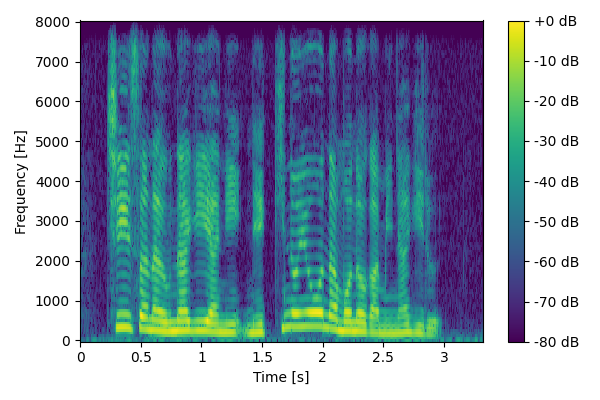
\includegraphics[width=\textwidth]{./figure/sec2/spectrogram_1.png}
        \caption{窓長12.5ms,シフト幅5ms}
        \label{sec2:fig:spectrogram1}
    \end{subfigure}
    \begin{subfigure}[b]{0.48\textwidth}
        \centering
        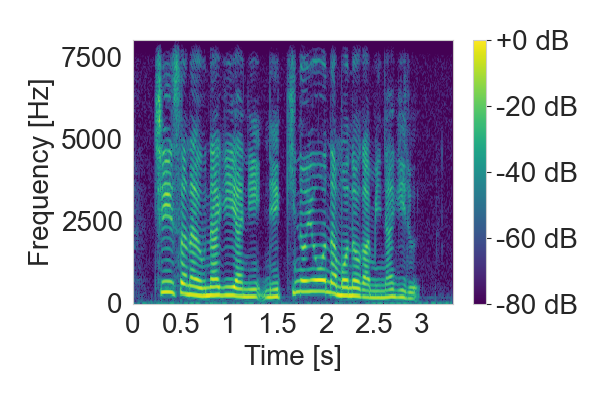
\includegraphics[width=\textwidth]{./figure/sec2/spectrogram_2.png}
        \caption{窓長25ms,シフト幅10ms}
        \label{sec2:fig:spectrogram2}
    \end{subfigure}

    \vspace{0.5cm}

    \begin{subfigure}[b]{0.48\textwidth}
        \centering
        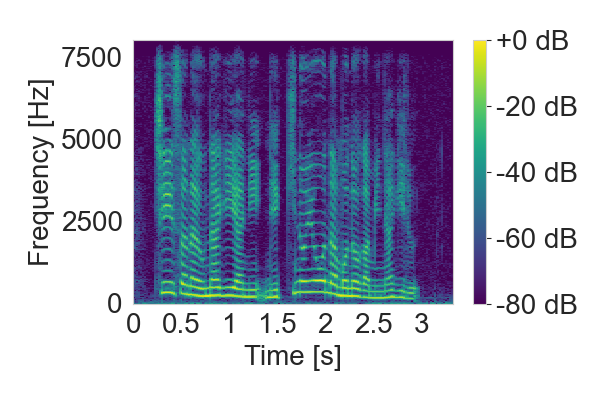
\includegraphics[width=\textwidth]{./figure/sec2/spectrogram_4.png}
        \caption{窓長50ms,シフト幅20ms}
        \label{sec2:fig:spectrogram3}
    \end{subfigure}
    \begin{subfigure}[b]{0.48\textwidth}
        \centering
        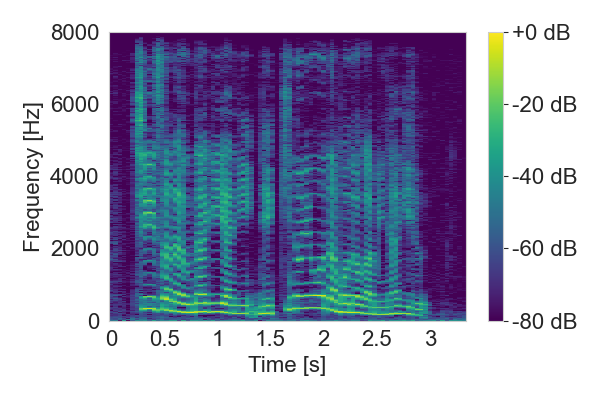
\includegraphics[width=\textwidth]{./figure/sec2/spectrogram_8.png}
        \caption{窓長100ms,シフト幅40ms}
        \label{sec2:fig:spectrogram4}
    \end{subfigure}
    \caption{「小さな鰻屋に,熱気のようなものがみなぎる」と発話した音声から計算された対数パワースペクトログラム}
    \label{sec2:fig:log_power_spectrograms}
\end{figure}

\subsection{メルスペクトログラム}
メルスペクトログラムは,パワースペクトログラムを人間の聴感特性を考慮したメル尺度に変換することによって得られる.周波数軸をメル尺度に変換する際,以下の式を用いる.
\begin{equation}
    \text{Mel}\lr{f} = 2595\log_{10} \lr{1 + \frac{f}{700}}
\end{equation}
メル尺度は,$\SI[]{1000}{Hz}$,$\SI[]{40}{dB}$の純音を$\SI[]{1000}{\text{mel}}$とする比率尺度である.メル尺度を用いることにより,低い周波数ほど細かく,高い周波数ほど荒い特徴量になる.メルスペクトログラムは,パワースペクトログラムに対してメルフィルタバンクを適用することによって得られる.メルフィルタバンクの数は任意に決定できるパラメータであり,メルスペクトログラムの周波数方向の次元はこれに一致する.音声合成においては,音声のサンプリング周波数を$\SI[]{16}{kHz}$とするとき,メルフィルタバンクの数を80とし,$\SI[]{8000}{Hz}$までの帯域に対して適用することが多い.「小さな鰻屋に,熱気のようなものがみなぎる」と発話した音声に対し,窓関数にハニング窓を用い,窓長25ms,シフト幅10msとしてパワースペクトログラムを計算した上で,80次元のメルフィルタバンクを適用して得られた対数メルスペクトログラムを,図~\ref{sec2:fig:melspectrogram}に示す.
\begin{figure}[bt]
    \centering
    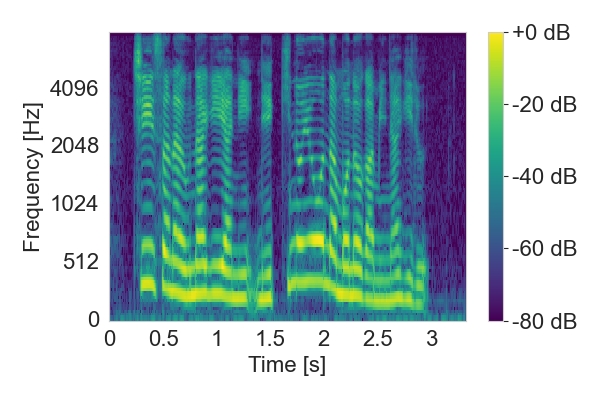
\includegraphics[height=70mm]{./figure/sec2/melspectrogram.png}
    \caption{「小さな鰻屋に,熱気のようなものがみなぎる」と発話した音声に対する対数メルスペクトログラム}
    \label{sec2:fig:melspectrogram}
\end{figure}
\clearpage

\section{深層学習}
深層学習とは,人間の神経細胞の仕組みを模擬したニューラルネットワークを用いる機械学習手法のことである.特に近年ではその層を深くしたディープニューラルネットワーク(Deep Neural Network; DNN)が用いられ,大量のパラメータによる表現力により,自然言語処理や画像処理,音声処理など様々な分野で成果を上げている.本章では,DNNの構成要素及び,構築したDNNの学習方法について説明する.
\subsection{DNNの構成要素}
\subsubsection{全結合層}
全結合層は,入力に対して線型変換を施す層である.全結合層への入力を$\bm{\inputLower} \in \realSet^{\dimUpper_{\text{in}}}$とすると,出力$\bm{\outputLower} \in \realSet^{\dimUpper_{\text{out}}}$は,
\begin{equation}
    \bm{\outputLower} = \fcLayerValue{\bm{\inputLower}}{\bm{\weightAndBias}} = \lr{\bm{\inputLower}^{\top} \bm{\weightUpper}}^{\top} + \bm{\biasLower}
\end{equation}
で与えられる.ここで,$\dimUpper_{\text{in}}, \dimUpper_{\text{out}}$は入出力の次元,$\bm{\weightUpper} \in \realSet^{\dimUpper_{\text{in}} \times \dimUpper_{\text{out}}}$は重み,$\bm{\biasLower} \in \realSet^{\dimUpper_{\text{out}}}$はバイアスであり,$\bm{\weightAndBias}$は重みとバイアスをまとめて表す変数とする.また,入力が行列$\bm{\inputUpper} \in \realSet^{\timeUpper \times \dimUpper_{\text{in}}}$である時,出力$\bm{Y} \in \realSet^{\timeUpper \times \dimUpper_{\text{out}}}$は,
\begin{equation}
    \bm{\outputUpper} = \fcLayerValue{\bm{\inputUpper}}{\bm{\weightAndBias}} = \bm{\inputUpper} \bm{\weightUpper} + \bm{\biasLower} \bm{1}^{\top}
\end{equation}
で与えられる.ここで,$\timeUpper$は系列長,$\bm{1} \in \{1\}^{\timeUpper}$は全成分が1のベクトルである.全結合層はDNN内部での特徴量の次元の変換や,最終層において所望の出力に次元を合わせるのに用いられる.

\subsubsection{畳み込み層}
畳み込み層は,入力に対して畳み込み演算を行う層である.1次元畳み込み層について,入力を$\bm{\inputUpper} \in \realSet^{\dimUpper_{\text{in}} \times \timeUpper_{\text{in}}}$,出力を$\bm{\outputUpper} \in \realSet^{\dimUpper_{\text{out}} \times \timeUpper_{\text{out}}}$とし,それぞれ$\dimLower$次元目,$\timeLower$番目の成分を$\inputLower_{\dimLower_{\text{in}}, \timeLower}, \outputLower_{\dimLower_{\text{out}}, \timeLower}$で表す.$\dimUpper_{\text{in}}, \dimUpper_{\text{out}}$は入出力の次元,$\timeUpper_{\text{in}}, \timeUpper_{\text{out}}$は入出力の系列長である.このとき,$\outputLower_{\dimLower_{\text{out}}, \timeLower}$は,
\begin{align}
    \outputLower_{\dimLower_{\text{out}}, \timeLower} = b_{\dimLower_{\text{out}}} + \sum_{\dimLower_{\text{in}} = 1}^{\dimUpper_{\text{in}}} \sum_{\kernelSizeLower = 1}^{\kernelSizeUpper} \inputLower_{\dimLower_{\text{in}}, \timeLower - \lrFloor{\frac{\kernelSizeUpper}{2}} + \kernelSizeLower - 1} \weightLower_{\dimLower_{\text{in}}, \dimLower_{\text{out}}, \kernelSizeLower}
\end{align}
で与えられる.ここで,$\kernelSizeUpper$はカーネルサイズ,$\weightLower_{\dimLower_{\text{in}}, \dimLower_{\text{out}}, \kernelSizeLower}$は入力の$\dimLower_{\text{in}}$次元目から出力の$\dimLower_{\text{out}}$次元目に割り当てられたカーネルの$\kernelSizeLower$番目の成分,$b_{\dimLower_{\text{out}}}$は出力の$\dimLower_{\text{out}}$次元目に割り当てられたバイアスである.上式より,1次元畳み込み層の$\timeLower$番目の出力は,$\timeLower$番目を中心としたカーネルサイズの範囲分の入力から計算されることがわかる($\kernelSizeUpper$は奇数を想定した).これより,畳み込み層は入力の局所的な特徴を抽出するのに適した層だと考えられる.1次元畳み込みはテキストや音声など,データの形状が$\lr{\dimUpper \times \timeUpper}$となっている時に用いられる.

これに加えて,カーネルを2次元配列とすれば2次元畳み込み層,3次元配列とすれば3次元畳み込み層となる.2次元畳み込み層は画像など,データの形状が$\lr{\dimUpper \times \heightUpper \times \widthUpper}$となっている場合に用いられる.ここで,$\heightUpper$は高さ,$\widthUpper$を表す.3次元畳み込み層は動画など,データの形状が$\lr{\dimUpper \times \heightUpper \times \widthUpper \times \timeUpper}$となっている場合に用いられる.

畳み込み層における主要なパラメータは3つある.1つ目はカーネルサイズであり,これによって考慮できる入力特徴量の範囲が定まる.2つ目はストライドであり,これによってカーネルのシフト幅を設定できる.3つ目はダイレーションであり,これは畳み込み演算において計算対象となる入力特徴量の間隔を表す.ダイレーションを大きくすることで,カーネルサイズが同じでも考慮できる入力特徴量の範囲を広げることが可能である.また,出力系列長$\timeUpper_{\text{out}}$を入力系列長$\timeUpper_{\text{in}}$の整数倍に保つには,上記のパラメータに対して適切なパディング長を指定する必要がある.図\ref{sec3:fig:conv_variations}に,ある入出力次元間における1次元畳み込み層の処理を示す.赤が入出力,青がカーネルを表している.図\ref{sec3:fig:conv1}は,カーネルサイズを3,ストライドとダイレーションを1とした場合であり,入力の両端に1ずつゼロパディングすることで,入出力の系列長が変わらないことを表している.図\ref{sec3:fig:conv2}は,カーネルサイズを5,ストライドとダイレーションを1とした場合であり,カーネルサイズが大きくなることで,出力1フレームを計算する際に考慮される入力の範囲が図\ref{sec3:fig:conv1}よりも広がることを表した.図\ref{sec3:fig:conv3}はカーネルサイズが3,ストライドが2,ダイレーションが1の場合であり,ストライドを2にしたことによって出力の系列長が入力よりも短くなることを表している.ここではパディングを1とすることで,入力に対して出力の系列長を$1/2$にできることを表した.図\ref{sec3:fig:conv4}はカーネルサイズが3,ストライドが1,ダイレーションが2の場合であり,ダイレーションを2とすることで,カーネルに対して入力が1フレーム飛ばしで計算されることを示した.

\begin{figure}[tb]
    \centering
    \begin{subfigure}[b]{0.48\textwidth}
        \centering
        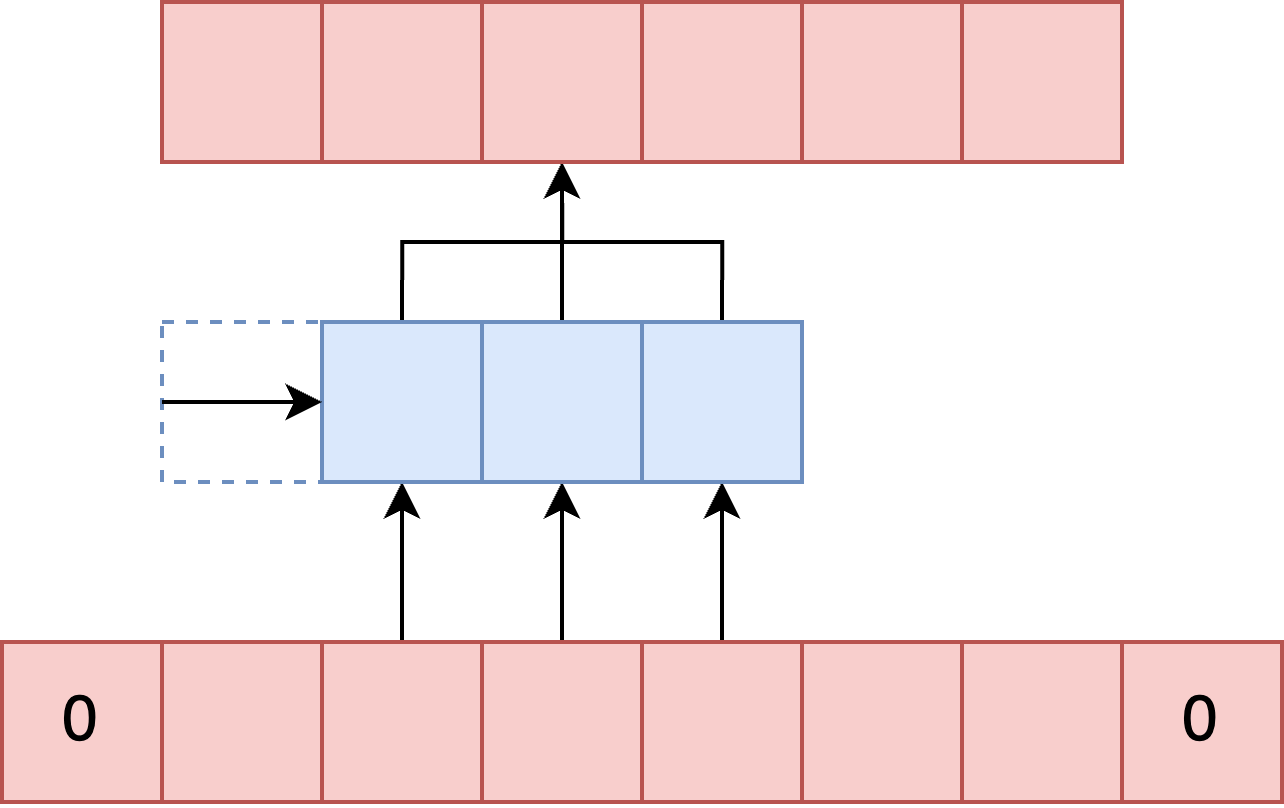
\includegraphics[height=4cm]{./figure/sec3/conv1.drawio.png}
        \caption{$\lr{\kernelSizeUpper, \strideUpper, \dilationUpper} = \lr{3, 1, 1}$}
        \label{sec3:fig:conv1}
    \end{subfigure}
    \begin{subfigure}[b]{0.48\textwidth}
        \centering
        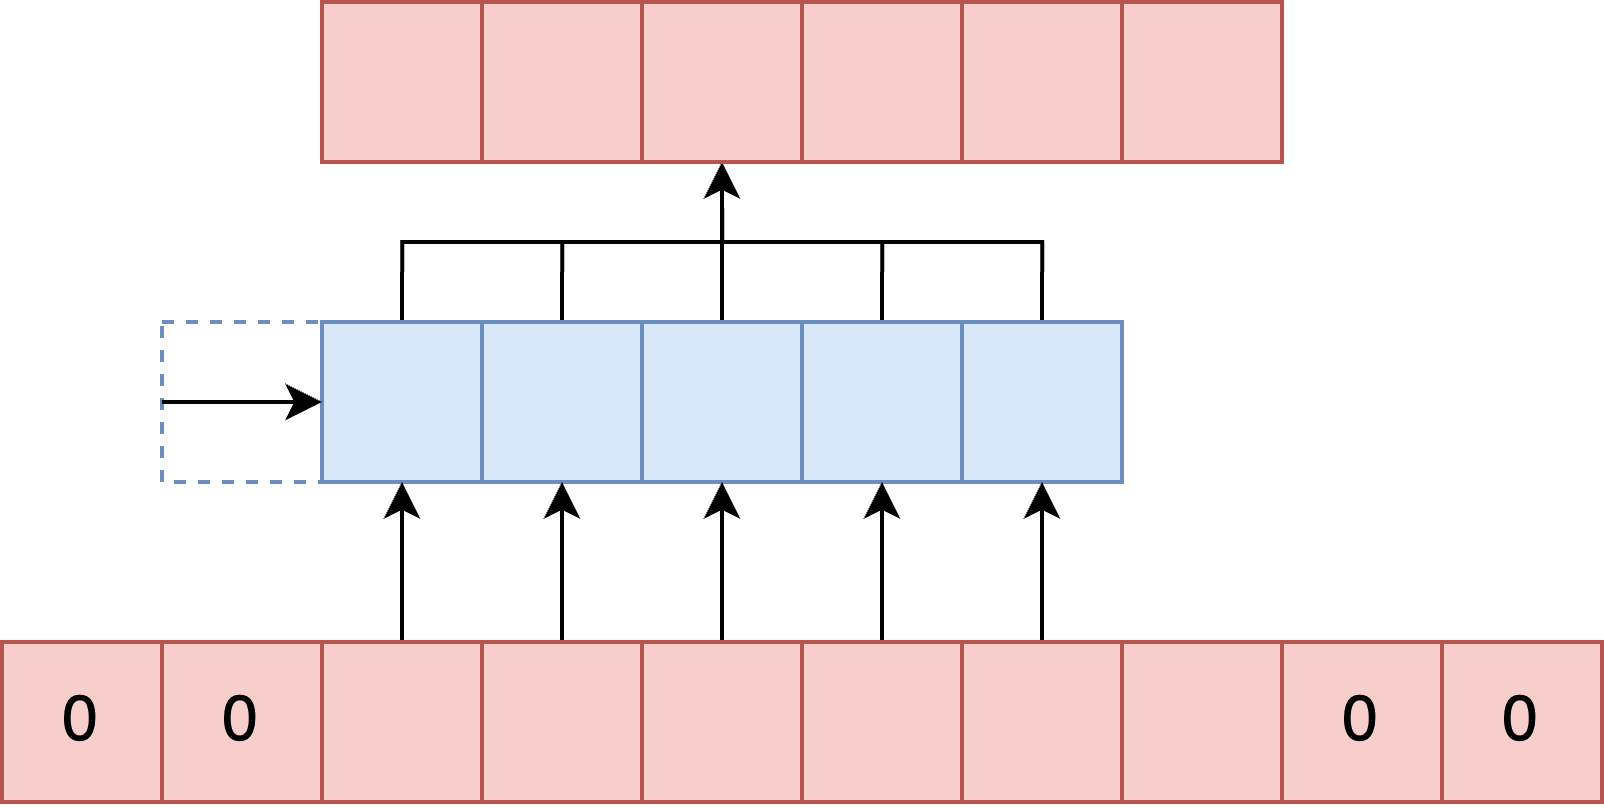
\includegraphics[height=4cm]{./figure/sec3/conv2.drawio.png}
        \caption{$\lr{\kernelSizeUpper, \strideUpper, \dilationUpper} = \lr{5, 1, 1}$}
        \label{sec3:fig:conv2}
    \end{subfigure}

    \vspace{0.5cm}

    \begin{subfigure}[b]{0.48\textwidth}
        \centering
        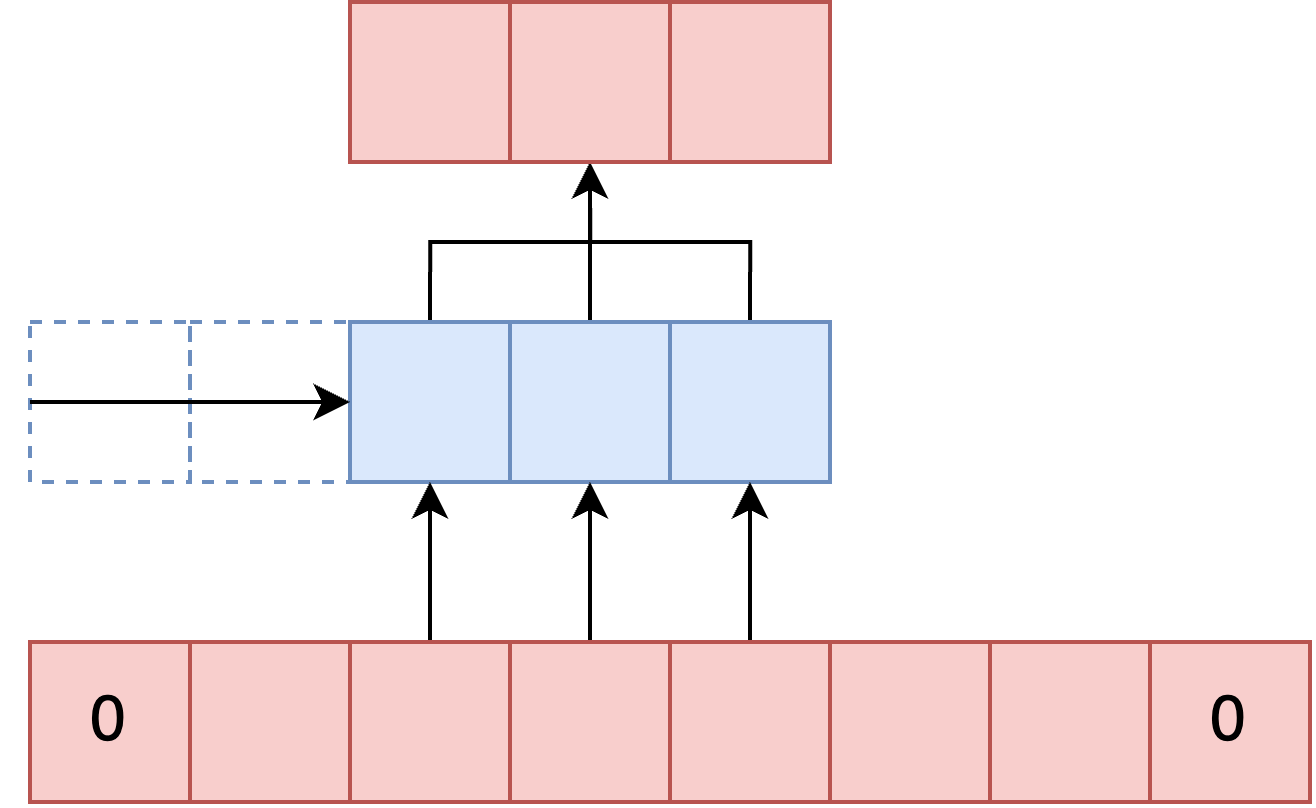
\includegraphics[height=4cm]{./figure/sec3/conv3.drawio.png}
        \caption{$\lr{\kernelSizeUpper, \strideUpper, \dilationUpper} = \lr{3, 2, 1}$}
        \label{sec3:fig:conv3}
    \end{subfigure}
    \begin{subfigure}[b]{0.48\textwidth}
        \centering
        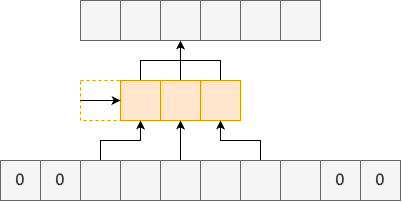
\includegraphics[height=4cm]{./figure/sec3/conv4.drawio.png}
        \caption{$\lr{\kernelSizeUpper, \strideUpper, \dilationUpper} = \lr{3, 1, 2}$}
        \label{sec3:fig:conv4}
    \end{subfigure}
    \caption{ある入出力次元間における1次元畳み込み層の処理.$\kernelSizeUpper$はカーネルサイズ,$\strideUpper$はストライド,$\dilationUpper$はダイレーションを表し,図中の0はパディング部を表す.}
    \label{sec3:fig:conv_variations}
\end{figure}

\subsubsection{転置畳み込み層}
転置畳み込み層は,畳み込み層の逆演算に対応する層であり,主に入力のアップサンプリングに使用される.図\ref{sec3:fig:tconv_variations}に,ある入出力次元間における1次元転置畳み込み層の処理を示す.赤が入出力,青がカーネルを表している.1次元転置畳み込み層では,$\timeLower$番目の入力とカーネルの積を計算し,その結果を$\timeLower$番目から$\timeLower + \kernelSizeUpper$番目までの出力とする.ここで$\kernelSizeUpper$はカーネルサイズである.また,複数の入力から計算された出力がオーバーラップする場合,これらは加算される.図\ref{sec3:fig:tconv1}は,カーネルサイズを4,ストライドを1とした場合の様子である.アップサンプリングを行いたい場合は,ストライドを2以上とすれば良い.図\ref{sec3:fig:tconv2}にカーネルサイズを4,ストライドを2とした場合を示す.この時,入力系列長が4であるのに対して,出力系列長が10まで拡大されていることがわかる.ここで,出力系列長を入力系列長の整数倍に保つためには,出力の両端の削除数を適切に設定する必要がある.上述の例では両端の削除数を1とすることで,出力系列長を入力系列長の2倍である8に調整できる.

\begin{figure}[tb]
    \centering
    \begin{subfigure}[b]{0.48\textwidth}
        \centering
        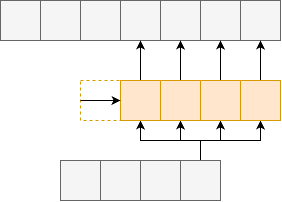
\includegraphics[height=4cm]{./figure/sec3/tconv1.drawio.png}
        \caption{$\lr{\kernelSizeUpper, \strideUpper} = \lr{4, 1}$}
        \label{sec3:fig:tconv1}
    \end{subfigure}
    \begin{subfigure}[b]{0.48\textwidth}
        \centering
        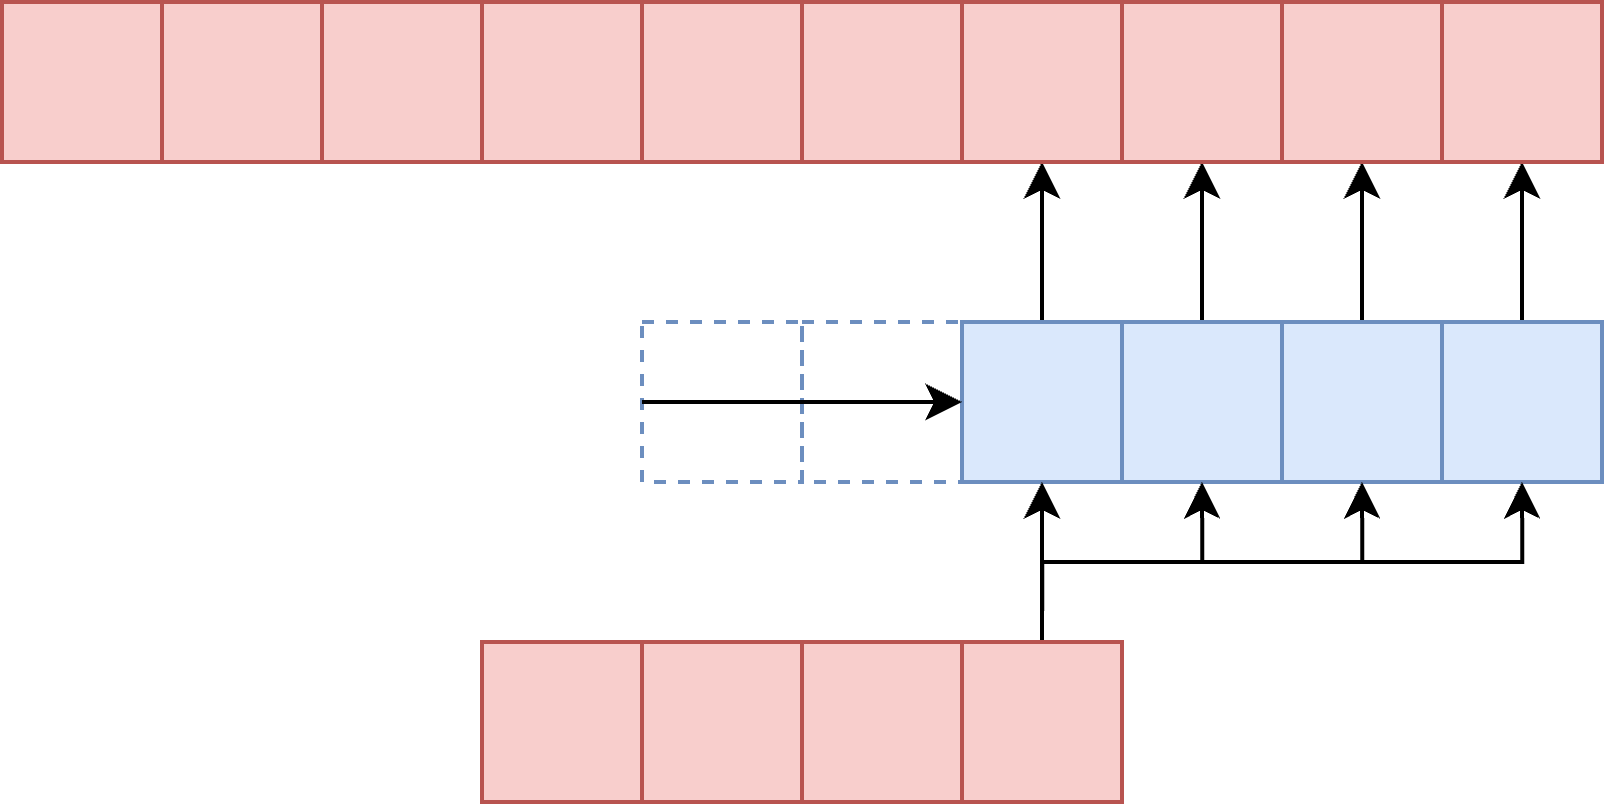
\includegraphics[height=4cm]{./figure/sec3/tconv2.drawio.png}
        \caption{$\lr{\kernelSizeUpper, \strideUpper} = \lr{4, 2}$}
        \label{sec3:fig:tconv2}
    \end{subfigure}
    \caption{ある入出力次元間における1次元転置畳み込み層の処理.$\kernelSizeUpper$はカーネルサイズ,$\strideUpper$はストライドを表す.}
    \label{sec3:fig:tconv_variations}
\end{figure}

\subsubsection{活性化関数}
活性化関数は,ニューラルネットワークの出力に非線形性を与えるための関数である.これにより,DNNは単純な線形変換だけでは表現できない複雑な入出力の関係を学習可能になる.以下,活性化関数への入力を$\inputLower \in \realSet$として,代表的なものを6つ述べる.また,本節で取り上げる活性化関数とその1階導関数のグラフを図\ref{sec3:fig:activations_and_their_prime}に示す.

1つ目は,シグモイド関数である.シグモイド関数は
\begin{equation}
    \sigmoid\lr{\inputLower} = \frac{1}{1 + \exp\lr{-\inputLower}}
\end{equation}
で与えられ,その1階導関数は
\begin{equation}
    \dv{\sigmoid\lr{\inputLower}}{x} = \frac{\exp\lr{-\inputLower}}{\lr{1 + \exp\lr{-\inputLower}}^{2}}
\end{equation}
となる.図\ref{sec3:fig:activations_prime}より,シグモイド関数の1階導関数の最大値は$\inputLower=0$における0.25であり,$\lrAbs{\inputLower}$が大きくなるのに伴って,1階導関数の値は小さくなることがわかる.DNNの各重みは損失関数の勾配を利用して更新されるが,特にシグモイド関数以前の層の重みにおける勾配は,シグモイド関数の1階導関数の値が乗算された結果となる.前述したように,シグモイド関数は1階導関数の値が小さくなりがちであるから,それ以前の層における勾配も小さくなり,重みの更新が進みづらくなる可能性がある.この問題を,勾配消失と呼ぶ.

2つ目は,$\tanh$関数である.$\tanh$は
\begin{equation}
    \tanh\lr{\inputLower} = \frac{\exp\lr{\inputLower} - \exp\lr{-\inputLower}}{\exp\lr{\inputLower} + \exp\lr{-\inputLower}}
\end{equation}
で与えられ,その1階導関数は
\begin{align}
    \dv{\tanh\lr{\inputLower}}{x} & = \frac{4}{\lr{\exp\lr{\inputLower} + \exp\lr{-\inputLower}}^{2}} \\
                                  & = \frac{1}{\cosh\lr{\inputLower}^{2}}
\end{align}
となる.$\tanh$の値域は$\lrClosedInterval{-1}{1}$となっており,図\ref{sec3:fig:activations_prime}より$\lrAbs{\inputLower}$が小さいところでは,シグモイド関数より1階導関数の値が大きくなることがわかる.しかし,$\lrAbs{\inputLower}$が大きくなればシグモイド関数と同様に1階導関数の値が小さくなることから,勾配消失のリスクを抱えていることがわかる.

3つ目は,$\relu$である.$\relu$は
\begin{equation}
    \relu\lr{\inputLower} = \max \lr{0, \inputLower}
\end{equation}
で与えられ,その1階導関数は
\begin{equation}
    \dv{\relu\lr{\inputLower}}{x} =
    \begin{cases}
        1 & \text{if $\inputLower > 0$}  \\
        0 & \text{if $\inputLower <= 0$}
    \end{cases}
\end{equation}
となる.ここで,$\relu$は本来$x = 0$で微分不可能であるが,便宜上$\dv*{\relu\lr{0}}{x} = 0$とした.$\relu$は入力が0以上であれば恒等写像として振る舞うが,0未満であれば0に写す.1階導関数は0あるいは1のみを取り,特に入力が正の値であれば常に1となることから,シグモイド関数や$\tanh$よりも勾配消失が起こりづらい.$\relu$は現在,標準的な活性化関数として広く用いられている.しかし,$\relu$への入力が0未満の値を取るとき,$\relu$入力についての出力の勾配は0になるから,$\relu$以前の層の重みが更新されず,学習が遅くなる可能性がある.

3つ目は,$\leakyRelu$\cite{maas2013rectifier}である.$\leakyRelu$は
\begin{equation}
    \leakyRelu\lr{\inputLower} =
    \begin{cases}
        \inputLower  & \text{if $\inputLower > 0$}  \\
        a\inputLower & \text{if $\inputLower <= 0$}
    \end{cases}
\end{equation}
で与えられ,その1階導関数は
\begin{equation}
    \dv{\leakyRelu\lr{\inputLower}}{x} =
    \begin{cases}
        1 & \text{if $\inputLower > 0$}  \\
        a & \text{if $\inputLower <= 0$}
    \end{cases}
\end{equation}
となる.ここで,$\leakyRelu$は本来$x = 0$で微分不可能であるが,便宜上$\dv*{\leakyRelu\lr{0}}{x} = a$とした.ReLUと比較すると,0未満の入力に対しても0でない値を出力し,1階導関数も0にならない点が異なっている.これにより,重みの更新が進まなくなるReLUの課題を解消した.

5つ目は,$\prelu$\cite{he2015delving}である.これは,$\leakyRelu$と似た活性化関数であるが,$\leakyRelu$のパラメータ$a$を学習可能にすることで,その他の層と合わせて最適化が可能となったことが特徴である.

6つ目は,$\gelu$\cite{hendrycks2016gaussian}である.$\gelu$は
\begin{equation}
    \gelu\lr{\inputLower} = \inputLower \Phi\lr{\inputLower}
\end{equation}
で与えられる.ここで,
\begin{equation}
    \Phi\lr{\inputLower} = P\lr{X \le \inputLower}, ~ X \sim \mathcal{N} \lr{0, 1}
\end{equation}
である.$\gelu$の1階導関数は,
\begin{equation}
    \dv{\gelu\lr{\inputLower}}{x} = \Phi\lr{\inputLower} + \frac{\inputLower}{\sqrt{2\pi}}\exp\lr{-\frac{\inputLower^{2}}{2}}
\end{equation}
となる.$\gelu$は,$\relu$が入力に対して0あるいは1を確定的にかける活性化関数と捉えた上で,これを入力に依存した確率的な挙動に変更したものである.
% 実際,$\binaryMaskLower \sim \text{Bernoulli}\lr{\Phi\lr{\inputLower}}$とすると,
% \begin{align}
%     \gelu\lr{\inputLower} & = \inputLower \Phi\lr{\inputLower}                                                             \\
%                           & = 1 \inputLower \cdot \Phi\lr{\inputLower} + 0 \inputLower \cdot \lr{1 - \Phi\lr{\inputLower}} \\
%                           & = \expectation{mx}
% \end{align}
% となり,$\gelu$の出力は確率的なバイナリマスク$\binaryMaskLower$を入力$\inputLower$にかけた,$mx$の期待値に等しいことがわかる.

\begin{figure}[tb]
    \centering
    \begin{subfigure}[b]{1.0\textwidth}
        \centering
        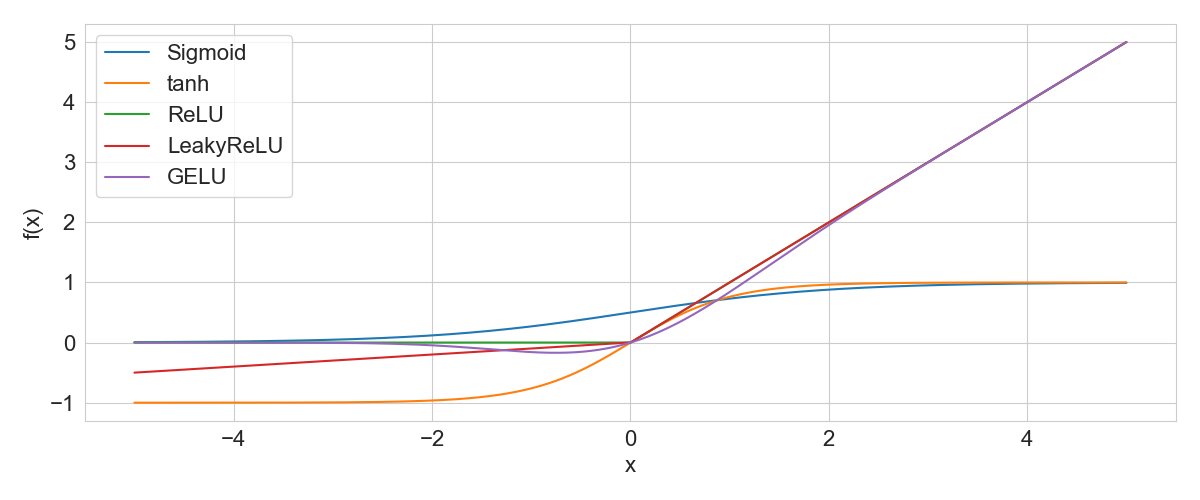
\includegraphics[width=160  mm]{./figure/sec3/activations.png}
        \caption{活性化関数}
        \label{sec3:fig:activations}
    \end{subfigure}
    \begin{subfigure}[b]{1.0\textwidth}
        \centering
        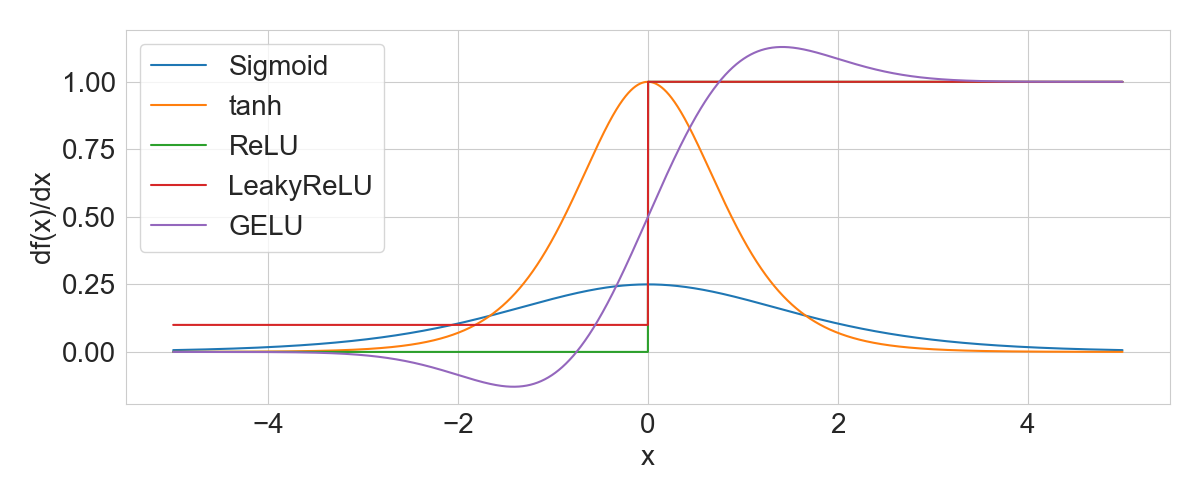
\includegraphics[width=160  mm]{./figure/sec3/activations_prime.png}
        \caption{活性化関数の1階導関数}
        \label{sec3:fig:activations_prime}
    \end{subfigure}
    \caption{活性化関数の例}
    \label{sec3:fig:activations_and_their_prime}
\end{figure}

\subsubsection{再帰型ニューラルネットワーク}
再帰型ニューラルネットワーク(Recurrent Neural Network; RNN)は,自身の過去の出力を保持し,それをループさせる再帰的な構造を持ったネットワークである.

近年よく用いられるRNNとして,長・短期記憶(Long Short-Time Memory; LSTM)\cite{hochreiter1997long}がある.LSTMは入力ゲート,忘却ゲート,出力ゲートの3つを持ち,これらゲートによってネットワーク内部の情報の取捨選択を行うことで,長い系列データからの学習を可能にした.LSTMのネットワーク内部で行われる計算を以下に示す.
\begin{gather}
    \bm{f}_{\timeLower} = \sigmoid\lr{\fcLayerValue{\bm{\inputLower}_{\timeLower}}{\bm{\weightAndBias}_{f, x}} + \fcLayerValue{\bm{h}_{\timeLower-1}}{\bm{\weightAndBias}_{f, h}}} \\
    \bm{i}_{\timeLower} = \sigmoid\lr{\fcLayerValue{\bm{\inputLower}_{\timeLower}}{\bm{\weightAndBias}_{i, \inputLower}} + \fcLayerValue{\bm{h}_{\timeLower-1}}{\bm{\weightAndBias}_{i, h}}} \\
    \tilde{\bm{c}}_{\timeLower} = \tanh\lr{\fcLayerValue{\bm{\inputLower}_{\timeLower}}{\bm{\weightAndBias}_{\tilde{c}, \inputLower}} + \fcLayerValue{\bm{h}_{\timeLower-1}}{\bm{\weightAndBias}_{\tilde{c}, h}}} \\
    \bm{o}_{\timeLower} = \sigmoid\lr{\fcLayerValue{\bm{\inputLower}_{\timeLower}}{\bm{\weightAndBias}_{o, \inputLower}} + \fcLayerValue{\bm{h}_{\timeLower-1}}{\bm{\weightAndBias}_{o, h}}} \\
    \bm{c}_{\timeLower} = \bm{f}_{\timeLower} \elemMul \bm{c}_{\timeLower-1} + \bm{i}_{\timeLower} \elemMul \tilde{\bm{c}}_{\timeLower} \\
    \bm{h}_{\timeLower} = \bm{o}_{\timeLower} \elemMul \tanh\lr{\bm{c}_{\timeLower}}
\end{gather}
ここで,$\bm{\inputLower}_{\timeLower} \in \realSet^{\dimUpper_{\text{in}}}$は時刻$\timeLower$の入力,$\bm{f}_{\timeLower} \in \lrsq{0, 1}^{\dimUpper_{\text{out}}}$は忘却ゲートの出力,$\bm{i}_{\timeLower} \in \lrsq{0, 1}^{\dimUpper_{\text{out}}}$は入力ゲートの出力,$\bm{c}_{\timeLower} \in \lrsq{-1, 1}^{\dimUpper_{\text{out}}}$は時刻$\timeLower$におけるセルの状態,$\bm{o}_{\timeLower} \in \lrsq{0, 1}^{\dimUpper_{\text{out}}}$は出力ゲートの出力,$\bm{h}_{\timeLower} \in \lrsq{-1, 1}^{\dimUpper_{\text{out}}}$は時刻$\timeLower$における隠れ状態,$\dimUpper_{\text{in}}, \dimUpper_{\text{out}}$は特徴量の次元を表す.また,$\concat{\cdot, \ldots, \cdot}$は入力された特徴量の次元方向の結合,$\elemMul$は要素積を表す.忘却ゲート出力$\bm{f}_{\timeLower}$が前時刻のセル状態$\bm{c}_{\timeLower - 1}$に含まれる情報の選択,入力ゲート出力$\bm{i}_{\timeLower}$が新たな入力$\tilde{\bm{c}}_{\timeLower}$に含まれる情報の選択に用いられ,$\bm{c}_{\timeLower}$が決まる.その後,出力ゲート出力$\bm{o}_{\timeLower}$が$\bm{c}_{\timeLower}$に含まれる情報の選択に用いられ,$\bm{h}_{\timeLower}$が決まる.

また,LSTMが3つのゲートを必要とするのに対し,ゲートを2つに減らすことでネットワークの軽量化を図ったのがゲート付き回帰型ユニット(Gated Recurrent Unit; GRU)\cite{cho2014learning}である.GRUはリセットゲートと更新ゲートの2つを用いて隠れ状態を更新する.GRUのネットワーク内部で行われる計算を以下に示す.
\begin{gather}
    \bm{z}_{\timeLower} = \sigmoid\lr{\fcLayerValue{\bm{\inputLower}_{\timeLower}}{\bm{\weightAndBias}_{z, \inputLower}} + \fcLayerValue{\bm{h}_{\timeLower-1}}{\bm{\weightAndBias}_{z, h}}} \\
    \bm{r}_{\timeLower} = \sigmoid\lr{\fcLayerValue{\bm{\inputLower}_{\timeLower}}{\bm{\weightAndBias}_{r, \inputLower}} + \fcLayerValue{\bm{h}_{\timeLower-1}}{\bm{\weightAndBias}_{r, h}}} \\
    \tilde{\bm{h}}_{\timeLower} = \tanh\lr{\fcLayerValue{\bm{\inputLower}_{\timeLower}}{\bm{\weightAndBias}_{\tilde{h}, \inputLower}} + \bm{r}_{\timeLower} \elemMul \fcLayerValue{\bm{h}_{\timeLower-1}}{\bm{\weightAndBias}_{\tilde{h}, h}}} \\
    \bm{h}_{\timeLower} = \lr{1 - \bm{z}_{\timeLower}} \elemMul \bm{h}_{\timeLower-1} + \bm{z}_{\timeLower} \elemMul \tilde{\bm{h}}_{\timeLower}
\end{gather}
ここで,$\bm{x}_{\timeLower} \in \realSet^{\dimUpper_{\text{in}}}$が時刻$\timeLower$における入力,$\bm{z}_{\timeLower} \in \lrsq{0, 1}^{\dimUpper_{\text{out}}}$が更新ゲートの出力,$\bm{r}_{\timeLower} \in \lrsq{0, 1}^{\dimUpper_{\text{out}}}$がリセットゲートの出力,$\bm{h}_{\timeLower} \in \lrsq{-1, 1}^{\dimUpper_{\text{out}}}$が時刻$\timeLower$における隠れ状態を表す.更新ゲート出力$\bm{z}_{\timeLower}$が$\bm{h}_{\timeLower - 1}$と$\tilde{\bm{h}}_{\timeLower}$に含まれる情報の選択,リセットゲート出力$\bm{r}_{\timeLower}$が$\bm{h}_{\timeLower - 1}$に含まれる情報の選択に用いられる.

\subsubsection{正規化層}
DNNの学習過程では学習の進行に伴って重みが変化するため,その度に各層への入力の分布が変わってしまう.これは内部共変量シフトと呼ばれ,ネットワークの学習を不安定にする原因となる.これに対し,バッチ正規化(Batch Normalization)\cite{ioffe2015batch}が有効である.バッチ正規化は,ミニバッチ内における入力特徴量の期待値と分散を次元ごとに計算し,これらを用いて入力特徴量を次元ごとに標準化するものである.ここで,バッチサイズを$\numUpper$,バッチ正規化への$D$次元の入力特徴量を$\bm{\inputLower}_{\numLower} \in \realSet^{\dimUpper} ~ \lr{\numLower = 1, \ldots, \numUpper}$,出力特徴量を$\bm{y}_{\numLower} \in \realSet^{\dimUpper} ~ \lr{\numLower = 1, \ldots, \numUpper}$とする.このとき,各$\numLower$に対し入力特徴量$\bm{\inputLower}_{\numLower}$の$\dimLower$次元目の成分を$\inputLower_{\numLower, \dimLower}$,出力特徴量$\bm{\outputLower}_{\numLower}$の$\dimLower$次元目の成分を$\outputLower_{\numLower, \dimLower}$とすると,$\outputLower_{\numLower, \dimLower}$は
\begin{align}
    \mean^{B}_{\dimLower}                      & = \frac{1}{\numUpper} \sum_{\numLower = 1}^{\numUpper} \inputLower_{\numLower, \dimLower}                                  \\
    \lr{\std^{B}_{\dimLower}}^{2}              & = \frac{1}{\numUpper} \sum_{\numLower = 1}^{\numUpper} \lr{\inputLower_{\numLower, \dimLower} - \mean^{B}_{\dimLower}}^{2} \\
    \tilde{\inputLower}_{\numLower, \dimLower} & = \frac{\inputLower_{\numLower, \dimLower} - \mean^{B}_{\dimLower}}{\sqrt{\lr{\std^{B}_{\dimLower}}^{2} + \epsilon}}       \\
    \outputLower_{\numLower, \dimLower}        & = \normScale_{\dimLower} \tilde{\inputLower}_{\numLower, \dimLower} +  \normShift_{\dimLower}
\end{align}
で与えられる.ここで,$\normScale_{\dimLower}, \normShift_{\dimLower}$は学習可能なスカラーであり,$\epsilon$はゼロ割を避けるためのスカラーである.バッチ正規化では$\normScale_{\dimLower}, \normShift_{\dimLower}$によって表現力を向上させており,実際
\begin{align}
    \normScale_{\dimLower} & = \sqrt{\lr{\std^{B}_{\dimLower}}^{2} + \epsilon} \\
    \beta_{\dimLower}      & = \mean^{B}_{\dimLower}
\end{align}
とすれば,標準化前の入力を再び得ることが可能である.学習時は,サンプルの標準化に用いる統計量とは別に,期待値の移動平均と不偏分散の移動平均を計算しておく.推論時は学習終了時に得られたこれら移動平均の値を用いるため,入力サンプルによらない挙動になる.

バッチ正規化はDNNの学習の安定化に貢献する一方,ミニバッチ全体における統計量を利用するため,バッチサイズが小さい場合はデータの分布を安定させることが難しくなる.また,テキストや音声といった系列長を持つデータを扱う場合,ミニバッチを構成するためにはゼロパディングによって系列長を揃える必要がある.この時,RNNの各ステップの出力に対しバッチ正規化を適用すると,ゼロパディングによって人為的に系列量を揃えているため,統計量が実際のデータの分布からかけ離れたものになる可能性がある.これらの課題に対し,ミニバッチ内の各サンプルごとに期待値と分散を求めて標準化する,レイヤー正規化(Layer Normalization)\cite{ba2016layer}がある.バッチ正規化のときと同様の表記を用いると,$\outputLower_{\numLower, \dimLower}$は
\begin{align}
    \mean^{L}_{\numLower}                      & = \frac{1}{\dimUpper} \sum_{\dimLower = 1}^{\dimUpper} \inputLower_{\numLower, \dimLower}                                  \\
    \lr{\std^{L}_{\numLower}}^{2}              & = \frac{1}{\dimUpper} \sum_{\dimLower = 1}^{\dimUpper} \lr{\inputLower_{\numLower, \dimLower} - \mean^{L}_{\numLower}}^{2} \\
    \tilde{\inputLower}_{\numLower, \dimLower} & = \frac{\inputLower_{\numLower, \dimLower} - \mean^{L}_{\numLower}}{\sqrt{\lr{\std^{L}_{\numLower}}^{2} + \epsilon}}       \\
    \outputLower_{\numLower, \dimLower}        & = \normScale_{\dimLower} \tilde{\inputLower}_{\numLower, \dimLower} +  \normShift_{\dimLower}
\end{align}
で与えられる.

上述したバッチ正規化およびレイヤー正規化は,特徴量を標準化することで学習を安定させる手法であった.一方,DNN内のある層の重みを再パラメータ化することで学習を安定させる手法として,重み正規化(Weight Normalization)\cite{salimans2016weight}がある.これは,ある層の重みベクトル$\bm{\weightLower}$を,
\begin{equation}
    \bm{\weightLower} = \frac{\bm{v}}{\lrTwoNorm{\bm{v}}} g
\end{equation}
のように単位ベクトル$\bm{v} / \lrTwoNorm{\bm{v}}$(ベクトルの向き)とスカラー$g$(ベクトルの長さ)に再パラメータ化するものである.学習時は重みの更新を$\bm{v}$と$g$で別々に行う.重み正規化は,バッチ正規化やレイヤー正規化と同様に学習の安定化に役立つが,計算に入力特徴量の系列長が依存しない.そのため,例えば音声波形など系列長が非常に長くなりがちなデータを扱う場合,計算コストを下げながら同様の効果を狙える手段だと考えられる.

\subsubsection{Transformer}
Transformer\cite{vaswani2017attention}は,自己注意機構(Self-Attention)を用いて,入力系列全体に渡る依存関係を捉えることができるニューラルネットワークである.特に,再帰的な計算を必要とするRNNと比較して,Transformerは並列計算のみ行うため,GPUによる計算の高速化が可能である.以下,入力特徴量を$\bm{\inputUpper} \in \realSet^{\timeUpper \times \dimUpper_{\text{model}}}$として,Transformerにおいて行われる計算を説明する.$T$は系列長,$\dimUpper_{\text{model}}$は特徴量の次元を表す.また,Transformer層の構造を図\ref{sec3:fig:transformer_layer}に示す.赤の平行四辺形が入出力,青の長方形が処理を表す.

\begin{figure}[bt]
    \centering
    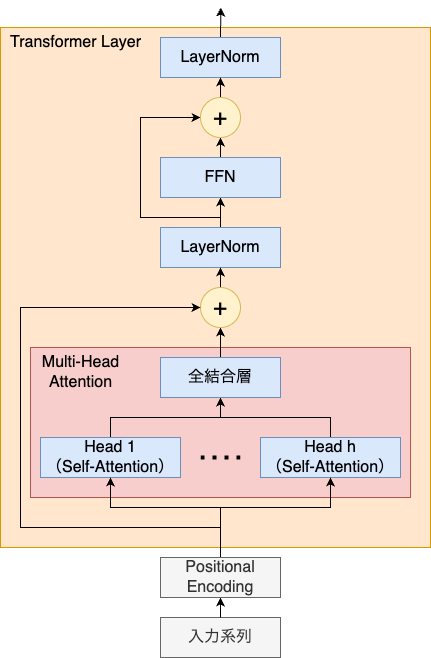
\includegraphics[width=150mm]{./figure/sec3/transformer.drawio.png}
    \caption{Transformer層の構造(赤い平行四辺形:入出力,青い長方形:処理)}
    \label{sec3:fig:transformer_layer}
\end{figure}

まず,Transformer層におけるSelf-Attentionの計算の流れを述べる.ここでは,はじめにクエリ$\bm{Q} \in \realSet^{\timeUpper \times \dimUpper_{k}}$,キー$\bm{K} \in \realSet^{\timeUpper \times \dimUpper_{k}}$,バリュー$\bm{V} \in \realSet^{\timeUpper \times \dimUpper_{v}}$の計算を行う.これは,
\begin{align}
    \bm{Q} & = \fcLayerValue{\bm{\inputUpper}}{\bm{\weightAndBias}_{Q}} \\
    \bm{K} & = \fcLayerValue{\bm{\inputUpper}}{\bm{\weightAndBias}_{K}} \\
    \bm{V} & = \fcLayerValue{\bm{\inputUpper}}{\bm{\weightAndBias}_{V}}
\end{align}
で与えられる.次に,クエリとキーを元にアテンション重みを求め,バリューに対する行列積を計算する.これは,
\begin{equation}
    \text{SA}\lr{\bm{Q}, \bm{K}, \bm{V}} = \text{softmax}\lr{\frac{\bm{Q}\bm{K}^\top}{\sqrt{\dimUpper_{k}}}} \bm{V}
\end{equation}
で与えられる.softmax関数は行方向に適用されるため,$\text{softmax}\lr{\bm{Q}\bm{K}^\top / \sqrt{\dimUpper_{k}}}$の各行ベクトルが,各クエリ$\bm{q}_{t} \in \realSet^{\dimUpper_{k}}$からキー$\bm{k}_{t} \in \realSet^{\dimUpper_{k}} ~ \lr{t = 1, \ldots, T}$に対する注意度になっている.

ここまでがSelf-Attentionの計算であったが,Transformer層ではSelf-Attentionを複数のヘッドで並列に計算し,各ヘッドの出力を結合して最終出力を得るMulti-Head Attentionが採用されている.これは,ヘッド数を$\numHeadUpper$とし,各ヘッド$\numHeadLower$におけるクエリ$\bm{Q}^{\numHeadLower} \in \realSet^{\timeUpper \times \frac{\dimUpper_{k}}{\numHeadUpper}}$,キー$\bm{K}^{\numHeadLower} \in \realSet^{\timeUpper \times \frac{\dimUpper_{k}}{\numHeadUpper}}$,バリュー$\bm{V}^{\numHeadLower} \in \realSet^{\timeUpper \times \frac{\dimUpper_{v}}{\numHeadUpper}}$によって計算された$\text{SA}\lr{\bm{Q}^{\numHeadLower}, \bm{K}^{\numHeadLower}, \bm{V}^{\numHeadLower}}$を用いて,
\begin{equation}
    \text{MHA}\lr{\bm{Q}, \bm{K}, \bm{V}} = \fcLayerValue{\concat{\text{SA}\lr{\bm{Q}^{1}, \bm{K}^{1}, \bm{V}^{1}}, \ldots, \text{SA}\lr{\bm{Q}^{\numHeadUpper}, \bm{K}^{\numHeadUpper}, \bm{V}^{\numHeadUpper}}}}{\bm{\weightAndBias}_{\text{MHA}}}
\end{equation}
で与えられる.Multi-Head Attention後は,残差結合とレイヤー正規化を適用する.すなわち,この出力$\bm{\outputUpper} \in \realSet^{\timeUpper \times \dimUpper_{\text{model}}}$は,
\begin{equation}
    \bm{\outputUpper} = \text{LayerNorm}\lr{\text{MHA}\lr{\bm{Q}, \bm{K}, \bm{V}} + \bm{\inputUpper}}
\end{equation}
で与えられる.その後,全結合層を通し,再度残差結合とレイヤー正規化を適用することでTransformer層最終出力を得る.すなわち,
\begin{equation}
    \bm{\outputUpper} = \text{LayerNorm}\lr{\fcLayerValue{\relu\lr{\fcLayerValue{\bm{\outputUpper}}{\bm{\weightAndBias}_{1}}}}{\bm{\weightAndBias}_{2}} + \bm{\outputUpper}}
\end{equation}
となる.Transformerは,Transformer層を多層積み重ねて構成される.

最後に,TransformerではRNNと違い,並列計算によって系列全体を1度に処理することが可能であるが,それと引き換えに入力の順序情報を考慮することができなくなる.これに対し,TransformerではPositional Encodingによって入力に位置情報を与える.Positional Encodingは$\sin$と$\cos$に基づいて,
\begin{equation}
    \text{PositionalEncoding}\lr{\timeLower, \dimLower} =
    \begin{cases}
        \sin \lr{\frac{\timeLower}{10000^{2\dimLower / \dimUpper_{\text{model}}}}} & \text{if $d \bmod 2 = 0$} \\
        \cos \lr{\frac{\timeLower}{10000^{2\dimLower / \dimUpper_{\text{model}}}}} & \text{if $d \bmod 2 = 1$}
    \end{cases}
\end{equation}
で与えられる.

\subsection{学習方法}
本節において,$\bm{\weightAndBias} \in \realSet^{\numUpper_{\text{model}}}$はDNNの重みとバイアスをまとめて表す変数とする.また,文章中では簡潔さを優先し,特別な理由がない限りは重みと呼ぶ.

\subsubsection{損失関数}
損失関数は,DNNによって推定された結果と正解値との間の誤差を求める関数のことであり,扱う問題によって様々である.例えば,回帰問題において用いられる関数の1つに,MAE(Mean Absolute Error)Lossがある.推定対象を$\bm{\outputLower} \in \realSet^{\dimUpper}$,DNNによる推定結果を$\hat{\bm{\outputLower}} \in \realSet^{\dimUpper}$とすると,MAE Lossは
\begin{equation}
    \lossFuncUpper_{\text{MAE}}\lr{\bm{\outputLower}, \hat{\bm{\outputLower}}} = \frac{1}{\dimUpper} \sum_{\dimLower = 1}^{\dimUpper}  \lrAbs{\outputLower_{\dimLower} - \hat{\outputLower}_{\dimLower}}
\end{equation}
で与えられる.また,推定対象が行列$\bm{\outputUpper} \in \realSet^{\timeUpper \times \dimUpper}$の場合,DNNによる推定結果を$\hat{\bm{\outputUpper}} \in \realSet^{\timeUpper \times \dimUpper}$とすると,MAE Lossは
\begin{equation}
    \lossFuncUpper_{\text{MAE}}\lr{\bm{\outputUpper}, \hat{\bm{\outputUpper}}} = \frac{1}{\timeUpper \dimUpper} \sum_{\timeLower = 1}^{\timeUpper} \sum_{\dimLower = 1}^{\dimUpper} \lrAbs{\outputLower_{\timeLower, \dimLower} - \hat{\outputLower}_{\timeLower, \dimLower}}
\end{equation}
で与えられる.

一方,分類問題において用いられる関数の1つに,Cross Entropy Lossがある.$\classUpper$クラス分類の問題について,予測対象を$\bm{\outputLower} \in \lrClosedInterval{0}{1}^{\classUpper}$,DNNによる予測値を$\hat{\bm{\outputLower}} \in \realSet^{\classUpper}$とすると,Cross Entropy Lossは
\begin{equation}
    \lossFuncUpper_{\text{CE}}\lr{\bm{\outputLower}, \hat{\bm{\outputLower}}} = - \sum_{\classLower = 1}^{\classUpper} y_{\classLower} \log \frac{\exp\lr{\hat{\outputLower}_{c}}}{\sum_{\indexLower = 1}^{C} \exp\lr{\hat{\outputLower}_{c}}}
\end{equation}
で与えられる.ここで,$\bm{\outputLower}$はクラスに対する確率分布であり,
\begin{equation}
    \sum_{\classLower = 1}^{\classUpper} y_{\classLower} = 1
\end{equation}
を満たす.実際は,正解となるクラスのみを1,それ以外を0としたOne-hotベクトルとされることが多い.また,予測値$\hat{\bm{\outputLower}}$は各クラスに対するスコアを表す値であり,ロジットと呼ばれる.予測対象が行列$\bm{\outputUpper} \in \lrClosedInterval{0}{1}^{\timeUpper \times \classUpper}$の場合,ロジットを$\hat{\bm{\outputUpper}} \in \realSet^{\timeUpper \times \dimUpper}$とすると,Cross Entropy Lossは
\begin{equation}
    \lossFuncUpper_{\text{CE}}\lr{\bm{\outputUpper}, \hat{\bm{\outputUpper}}} = - \frac{1}{\timeUpper} \sum_{\timeLower = 1}^{\timeUpper} \sum_{\classLower = 1}^{\classUpper} y_{\timeLower, \classLower} \log \frac{\exp\lr{\hat{\outputLower}_{\timeLower, \classLower}}}{\sum_{\indexLower = 1}^{C} \exp\lr{\hat{\outputLower}_{\timeLower, \indexLower}}}
\end{equation}
で与えられる.

\subsubsection{勾配降下法}
\label{sec3:sec:gradient_descent}
勾配降下法(Gradient Descent)は,損失関数の重みについての勾配を利用して,損失関数の値を最小化するようにDNNを最適化するアルゴリズムである.ここで,学習データセットを$\datasetTrain = \lrc{\lr{\bm{\inputLower}_{\numLower}, \bm{\outputLower}_{\numLower}}}_{\numLower = 1}^{\numUpper}$とする.各$\numLower$に対し,$\bm{\inputLower}_{\numLower} \in \realSet^{\dimUpper_{\text{in}}}$はDNNへの入力, $\bm{\outputLower}_{\numLower} \in \realSet^{\dimUpper_{\text{out}}}$は予測対象を表す.DNNは$f: \realSet^{\dimUpper_{\text{in}}} \to \realSet^{\dimUpper_{\text{out}}}$で表し,予測値を$\hat{\bm{\outputLower}}_{\numLower} = f\lr{\bm{\inputLower}_{\numLower}; \bm{\weightAndBias}}$とする.損失関数は$\lossFuncUpper: \realSet^{\dimUpper_{\text{out}}} \times \realSet^{\dimUpper_{\text{out}}} \to \realSet$とし,$\mathcal{\lossFuncUpper}: \realSet^{\numUpper_{\text{model}}} \to \realSet$を,
\begin{equation}
    \mathcal{\lossFuncUpper}\lr{\bm{\weightAndBias}; \mathcal{\indexUpper}} = \frac{1}{\card{\mathcal{\indexUpper}}} \sum_{\indexLower \in \mathcal{\indexUpper}} \lossFuncUpper\lr{\bm{\outputLower}_{\indexLower}, \hat{\bm{\outputLower}}_{\indexLower}} = \frac{1}{\card{\mathcal{\indexUpper}}} \sum_{\indexLower \in \mathcal{\indexUpper}} \lossFuncUpper\lr{\bm{\outputLower}_{\indexLower}, f\lr{\bm{\inputLower}_{\indexLower}; \bm{\weightAndBias}}}
\end{equation}
で定義する.ここで,$\mathcal{\indexUpper} \subset \{1, \ldots, N\}$は各サンプルに対するインデックスの部分集合,$\card{\cdot}$は集合の濃度を表す.すなわち,$\mathcal{\lossFuncUpper}$は学習データ$\left\{\lr{\bm{\inputLower}_{\indexLower}, \bm{\outputLower}_{\indexLower}}\right\}_{\indexLower \in \indexUpper} \subset \mathcal{D}_{\text{train}}$に対する損失を,DNNの重み$\bm{\weightAndBias}$の関数として扱うものである.上の表記を用いれば,DNNの最適化問題は
\begin{equation}
    \min_{\bm{\weightAndBias} \in \realSet^{\numUpper_{\text{model}}}} \mathcal{\lossFuncUpper}\lr{\bm{\weightAndBias}; \{1, \ldots, N\}}
\end{equation}
と表される.この最適化問題に対し,勾配降下法による重み$\bm{\weightAndBias}$の更新は,
\begin{equation}
    \label{sec3:eq:normal_gradient_descent}
    \bm{\weightAndBias}_{\iter} = \bm{\weightAndBias}_{\iter - 1} - \learningRate \nabla_{\bm{\weightAndBias}} \mathcal{\lossFuncUpper}\lr{\bm{\weightAndBias}_{\iter - 1}; \mathcal{I}_{\iter}}
\end{equation}
で与えられる.ここで,$\iter \in \naturalSet$は学習におけるイテレーション,$\learningRate \in \lrLeftClosedInterval{0}{\infty}$は学習率を表す.

勾配降下法には,3種類の方法がある\cite{zhang2019gradient}.1つ目は,バッチ勾配降下法である.これは,
\begin{equation}
    \bm{\weightAndBias}_{\iter} = \bm{\weightAndBias}_{\iter - 1} - \learningRate \nabla_{\bm{\weightAndBias}} \mathcal{\lossFuncUpper}\lr{\bm{\weightAndBias}_{\iter - 1}; \{1, \ldots, N\}}
\end{equation}
で与えられる.すなわち,各イテレーションで学習データ全てを用いる方法である.各サンプルのノイズの影響が低減されることで安定した学習が期待できるが,計算コストが高い.2つ目は,確率的勾配降下法である.これは,ランダムに選択された$n_{\iter} \in \{1, \ldots, N\}$に対し,
\begin{equation}
    \bm{\weightAndBias}_{\iter} = \bm{\weightAndBias}_{\iter - 1} - \learningRate \nabla_{\bm{\weightAndBias}} \mathcal{\lossFuncUpper}\lr{\bm{\weightAndBias}_{\iter - 1}; \{n_{\iter}\}}
\end{equation}
で与えられる.すなわち,各イテレーションで単一サンプルのみを用いる方法である.計算コストが下がるが,各サンプルのノイズの影響が大きくなることで学習が不安定になる可能性がある.3つ目は,ミニバッチ勾配降下法である.これは,$1 < \card{\mathcal{I}_{\iter}} < N$を満たすランダムに選択された$\mathcal{I}_{\iter} \subsetneq \{1, \ldots, N\}$に対し,
\begin{equation}
    \bm{\weightAndBias}_{\iter} = \bm{\weightAndBias}_{\iter - 1} - \learningRate \nabla_{\bm{\weightAndBias}} \mathcal{\lossFuncUpper}\lr{\bm{\weightAndBias}_{\iter - 1}; \mathcal{I}_{\iter}}
\end{equation}
で与えられる.これより,各イテレーションで2つ以上のサンプルからなる学習データセットの真部分集合を用いる方法だと言える.バッチ勾配降下法と確率的勾配降下法の間をとった方法であり,DNNの学習においては一般にミニバッチ勾配降下法が用いられる.ここで,ミニバッチに含まれるサンプルの数をバッチサイズと呼ぶ.

また,確率的勾配降下法やミニバッチ勾配降下法では,サンプルを学習データセットからランダムに非復元抽出する.ここで,毎回のサンプリングされた学習データに対する処理は1イテレーションとカウントし,学習データセットを一度全て使い切ることは1エポックとカウントする.実際には,データセットの総サンプル数$N$に対してバッチサイズを決定することで1エポックあたりの総イテレーション数は決まり,最大エポック数を設定して学習を回すこととなる.

\subsubsection{正則化}
DNNは大量のパラメータにより高い表現力を持つが,その分学習データに過剰に適合し,未知データに対する汎化性能が低いモデルとなる,過学習を引き起こす可能性がある.正則化は,このようなDNNの過学習を防ぐための手段である.以下,具体的な方法を3つ述べる.

1つ目は,L2正則化である.これは,$\mathcal{\lossFuncUpper}\lr{\bm{\weightAndBias}; \mathcal{\indexUpper}}$を
\begin{equation}
    \label{sec3:eq:l2_reg}
    \mathcal{\lossFuncUpper}\lr{\bm{\weightAndBias}; \mathcal{\indexUpper}} = \frac{1}{\card{\mathcal{\indexUpper}}} \sum_{\indexLower \in \mathcal{\indexUpper}} \lossFuncUpper\lr{\bm{\outputLower}_{\indexLower}, f\lr{\bm{\inputLower}_{\indexLower}; \bm{\weightAndBias}}} + \frac{\regConst}{2} \lrTwoNorm{\bm{\weightAndBias}}^{2}
\end{equation}
とすることで与えられる.ここで,$\regConst \in \lrLeftClosedInterval{0}{\infty}$は正則化の程度を調整するパラメータである.これより,L2正則化は損失関数の値に$\lrTwoNorm{\bm{\weightAndBias}}^{2}$を加算することで,重み$\bm{\weightAndBias}$のL2ノルムが過大になることを防ぐ方法だと言える.

2つ目は,Weight Decayである.これは,重みの更新式を
\begin{equation}
    \label{sec3:eq:weight_decay}
    \bm{\weightAndBias}_{\iter} = \bm{\weightAndBias}_{\iter - 1} - \learningRate \nabla_{\bm{\weightAndBias}} \mathcal{\lossFuncUpper}\lr{\bm{\weightAndBias}_{\iter - 1}; \mathcal{I}_{\iter}} - \regConst' \bm{\weightAndBias}
\end{equation}
とすることで与えられる.ここで,$\regConst' \in \lrLeftClosedInterval{0}{\infty}$は正則化の程度を調整するパラメータである.これより,Weight Decayは重み$\bm{\weightAndBias}$の絶対値が過大になることを防ぐ手法だと言える.

3つ目は,Dropout\cite{srivastava2014dropout}である.Dropoutは,学習時に特徴量の一部を0に落とす手法である.一方,推論時は恒等写像となり,学習時と挙動が変わる.Dropoutへの入力を$\bm{\inputLower} \in \realSet^{\dimUpper_{\text{in}}}$,特徴量を0に落とす確率を$p \in \lr{0, 1}$とすると,学習時のDropout出力$\bm{\outputLower}_{\text{train}} \in \realSet^{\dimUpper_{\text{out}}}$および推論時のDropout出力$\bm{\outputLower}_{\text{infer}} \in \realSet^{\dimUpper_{\text{out}}}$は,
\begin{align}
    \bm{\outputLower}_{\text{train}} & = \frac{\bm{x} \elemMul \bm{m}}{1 - p} \label{sec3:eq:regularization_dropout_training_output} \\
    \bm{\outputLower}_{\text{infer}} & = \bm{x}
\end{align}
で与えられる.ここで,$\bm{m} \in \{0, 1\}^{\dimUpper_{\text{in}}}$は各成分$m_{\dimLower}$が確率$1 - p$で1,確率$p$で0をとる確率変数である.式\eqref{sec3:eq:regularization_dropout_training_output}より,学習時はDropout出力を$1 / \lr{1 - p}$倍していることがわかる.この理由は,学習時の出力の期待値と推論時の出力を一致させるためである.実際,確率変数$\bm{m}$の従う確率分布上で$\bm{\outputLower}_{\text{train}}$の期待値をとれば,
\begin{align}
    \expectation{\bm{\outputLower}_{\text{train}}} & = \expectation{\frac{\bm{x} \elemMul \bm{m}}{1 - p}}             \\
                                                   & = \frac{\bm{x}}{1 - p} \elemMul \expectation{\bm{m}}             \\
                                                   & = \frac{\bm{x}}{1 - p} \elemMul \lr{1 - p ~ \cdots ~ 1 - p}^\top \\
                                                   & = \bm{x} = \bm{\outputLower}_{\text{infer}}
\end{align}
となる.Dropoutは学習時に一部のニューロンを落とすことで,実質的に異なるネットワークを学習させていると考えることができる.よって,学習時の出力の期待値に推論時の出力を一致させることは,異なるネットワークから得られた出力の期待値をとり,アンサンブルモデルとして推論時の出力を得ていると解釈できる.

3つ目は,Early Stoppingである.Early Stoppingは,検証データに対する損失の増加を監視し,設定したエポック数だけ増加し続けた場合に学習を停止する手法である.これにより,学習データに対する過度なフィッティングを防止する.

\subsubsection{最適化手法}
% 時間あればadamがmomentamやrmspropの発展として解釈できることを述べても良い.
\label{sec3:sec:optimizer}
\ref{sec3:sec:gradient_descent}節において,DNNの重みが勾配降下法によって最適化されることを述べた.ここで,通常の勾配降下法に代わり,近年よく用いられる最適化手法としてAdam\cite{kingma2014adam}がある.Adamの計算過程をアルゴリズム\ref{sec3:algo:adam}に示す.ここで,$\bm{g}_{\iter} \in \realSet^{\numUpper_{\text{model}}}$は勾配の一次モーメント,$\bm{m}_{\iter} \in \realSet^{\numUpper_{\text{model}}}$が勾配の一次モーメントの指数移動平均,$\bm{v}_{\iter} \in \realSet^{\numUpper_{\text{model}}}$が勾配の二次モーメントの指数移動平均である.$\hat{\bm{m}}_{\iter}$および$\hat{\bm{v}}_{\iter}$はそれぞれ,$\bm{m}_{\iter}$および$\bm{v}_{\iter}$の初期値が0であることに起因するバイアスを防ぐための計算を行った結果である.また,$\optimEmaConst_{1}, \optimEmaConst_{2} \in \lrClosedInterval{0}{1}$が,指数移動平均の程度を調整するパラメータである.
\begin{algorithm}
    \caption{Adam}
    \label{sec3:algo:adam}
    \begin{algorithmic}[1]
        \State \textbf{Input:} $\learningRate$, $\optimEmaConst_{1}$, $\optimEmaConst_{2}$, $\regConst$, $\bm{\weightAndBias}_{0}$, $L\lr{\bm{\weightAndBias}}$
        \State $\bm{m}_{0} = 0$, $\bm{v}_{0} = 0$
        \For{$\iter = 1$ to \texttt{...}}
        \State $\bm{g}_{\iter} = \nabla_{\bm{\weightAndBias}} \mathcal{\lossFuncUpper}\lr{\bm{\weightAndBias}_{\iter - 1}; \mathcal{I}_{\iter}} + \regConst \bm{\weightAndBias}_{\iter-1}$
        \State $\bm{m}_{\iter} = \optimEmaConst_{1} \bm{m}_{\iter-1} + \lr{1 - \optimEmaConst_{1}} \bm{g}_{\iter}$
        \State $\bm{v}_{\iter} = \optimEmaConst_{2} \bm{v}_{\iter-1} + \lr{1 - \optimEmaConst_{2}} \bm{g}_{\iter} \elemMul \bm{g}_{\iter}$
        \State $\tilde{\bm{m}}_{\iter} = \bm{m}_{\iter} / \lr{1 - \optimEmaConst_{1}^{\iter}}$
        \State $\tilde{\bm{v}}_{\iter} = \bm{v}_{\iter} / \lr{1 - \optimEmaConst_{2}^{\iter}}$
        \State $\bm{\weightAndBias}_{\iter} = \bm{\weightAndBias}_{\iter-1} - \learningRate \tilde{\bm{m}}_{\iter} / \lr{\sqrt{\tilde{\bm{v}}_{\iter}} + \epsilon}$
        \EndFor
        \State \textbf{Return} $\bm{\weightAndBias}_{\iter}$
    \end{algorithmic}
\end{algorithm}
ここで,Adamでは正則化としてL2正則化を採用したが,Weight Decayを採用した最適化手法としてAdamW\cite{loshchilov2017decoupled}がある.AdamWの計算過程をアルゴリズム\ref{sec3:algo:adamw}に示す.正則化がL2正則化からWeight Decayに変わった点以外は同じである.
\begin{algorithm}
    \caption{AdamW}
    \label{sec3:algo:adamw}
    \begin{algorithmic}[1]
        \State \textbf{Input:} $\learningRate$, $\optimEmaConst_{1}$, $\optimEmaConst_{2}$, $\regConst$, $\bm{\weightAndBias}_{0}$, $L\lr{\bm{\weightAndBias}}$
        \State $\bm{m}_{0} = 0$, $\bm{v}_{0} = 0$
        \For{$\iter = 1$ to \texttt{...}}
        \State $\bm{g}_{\iter} = \nabla_{\bm{\weightAndBias}} \mathcal{\lossFuncUpper}\lr{\bm{\weightAndBias}_{\iter - 1}; \mathcal{I}_{\iter}}$
        \State $\bm{m}_{\iter} = \optimEmaConst_{1} \bm{m}_{\iter - 1} + \lr{1 - \optimEmaConst_{1}} \bm{g}_{\iter}$
        \State $\bm{v}_{\iter} = \optimEmaConst_{2} \bm{v}_{\iter - 1} + \lr{1 - \optimEmaConst_{2}} \bm{g}_{\iter} \elemMul \bm{g}_{\iter}$
        \State $\tilde{\bm{m}}_{\iter} = \bm{m}_{\iter} / \lr{1 - \optimEmaConst_{1}^{\iter}}$
        \State $\tilde{\bm{v}}_{\iter} = \bm{v}_{\iter} / \lr{1 - \optimEmaConst_{2}^{\iter}}$
        \State $\bm{\weightAndBias}_{\iter} = \bm{\weightAndBias}_{\iter - 1} - \learningRate \tilde{\bm{m}}_{\iter} / \lr{\sqrt{\tilde{\bm{v}}_{\iter}} + \epsilon} - \regConst \bm{\weightAndBias}$
        \EndFor
        \State \textbf{Return} $\bm{\weightAndBias}_{\iter}$
    \end{algorithmic}
\end{algorithm}

\subsubsection{学習率のスケジューリング}
学習率のスケジューリングは,学習率$\learningRate$の値自体を学習の進行に伴って変更するものである.これは,より安定した学習を促したり,より早く学習を収束させたりするのに役立つ手段である.以下,3つのスケジューラを例として述べる.また,各スケジューラを用いた場合における学習率の遷移を図~\ref{sec3:fig:lr_scheduler}に示す.

1つ目は,StepLRSchedulerである.これは,初期学習率を$\learningRate_{0}$として,エポック$\epoch$における学習率$\learningRate_{\epoch}$を
\begin{equation}
    \learningRate_{\epoch} = \learningRate_{0} \gamma^{\left\lfloor \epoch / \text{stepSize} \right\rfloor}
\end{equation}
で与えるスケジューラである.これは,学習が$\text{stepSize}$エポック進むごとに学習率を$\gamma$倍することで,学習率を段階的に変化させる.シンプルで分かりやすいが,学習率の変化が不連続的になる.

2つ目は,ExponentialLRSchedulerである.これは,$\learningRate_{\epoch}$を
\begin{equation}
    \learningRate_{\epoch} = \learningRate_{0} \exp \lr{ -\gamma \epoch }
\end{equation}
で与えるスケジューラである.学習が1エポック進むごとに学習率を指数関数的に変化させるため,StepLRSchedulerと比較して変化が連続的である.

3つ目は,Cosine Annealing with Warmupである.これは,$\learningRate_{\epoch}$を
\begin{equation}
    \learningRate_{\epoch} =
    \begin{cases}
        \learningRate_{\text{min}} + \lr{ \frac{\epoch}{\text{WarmupSteps}} } \lr{\learningRate_{\text{max}} - \learningRate_{\text{min}}}                                                                                & \text{if $\epoch < \text{WarmupSteps}$}   \\
        \learningRate_{\text{min}} + \frac{1}{2} \lr{\learningRate_{\text{max}} - \learningRate_{\text{min}}} \lr{ 1 + \cos \lr{ \frac{\lr{\epoch - \text{WarmupSteps}}\pi}{\epoch_{\text{max}} - \text{WarmupSteps}} } } & \text{if $\epoch \ge \text{WarmupSteps}$}
    \end{cases}
\end{equation}
で与えるスケジューラである.ここで,$\learningRate_{\text{min}}$は最小学習率,$\learningRate_{\text{max}}$は最大学習率,$\epoch_{\text{max}}$は最大エポックである.$\text{WarmupSteps}$は学習率を$\learningRate_{\text{min}}$から$\learningRate_{\text{max}}$まで線形に増加させるのにかけるエポック数を指定するパラメータである.エポック数が$\text{WarmupSteps}$以上となれば,$\cos$関数に従って学習率を減衰させる.Cosine Annealing with Warmupは不安定になりがちな学習初期に学習率が低い状態から開始して,徐々に学習率を大きくすることで解の十分な探索を可能にし,その後再び学習率を小さくすることで学習の収束を促すスケジューラである.

\begin{figure}[bt]
    \centering
    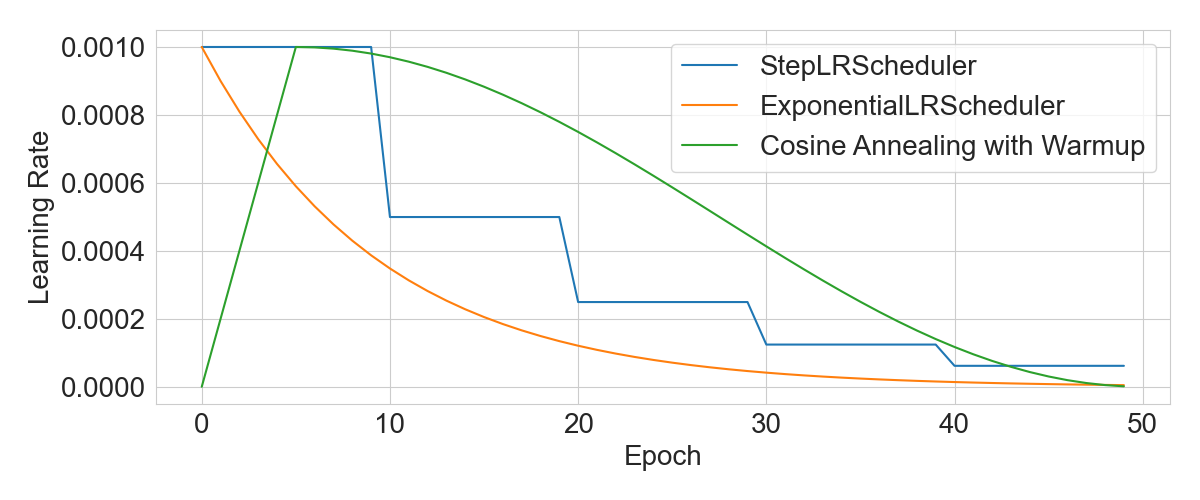
\includegraphics[height=70mm]{./figure/sec3/lr_scheduler.png}
    \caption{スケジューラによる学習率の変化}
    \label{sec3:fig:lr_scheduler}
\end{figure}

\subsubsection{誤差逆伝播法}
\label{sec3:sec:backpropagation}
誤差逆伝播法は,DNNの各重みについての損失関数の勾配を,出力から入力へと遡る方向に計算するアルゴリズムである.ここでは例として,全結合層と活性化関数のみからなる$\numUpper_{\text{layer}}$層のDNNを構築し,ミニバッチ勾配降下法によって最適化する場面を考える\cite{higham2019deep}.

まず,$\weightLower_{p, q}^{n} \in \realSet$を$n - 1$層目の$p$番目のニューロンから$n$層目の$q$番目のニューロンに割り当てられた重み,$b_{p}^{n} \in \realSet$を$n$層目の$p$番目のニューロンに割り当てられたバイアスとすると,$n$層目の$p$番目のニューロンにおける出力$a_{p}^{n} \in \realSet$は,
\begin{equation}
    \label{sec3:eq:output_before_act}
    a_{p}^{n} = b_{p}^{n} + \sum_{q = 1}^{\dimUpper_{n - 1}} \weightLower_{q, p}^{n} o_{q}^{n - 1}
\end{equation}
で与えられる.ここで,$\dimUpper_{n - 1}$は$n - 1$層目の全結合層の次元(総ニューロン数),$o_{q}^{n - 1} \in \realSet$は$n - 1$層目の$q$番目のニューロンにおける出力$a_{q}^{n - 1}$に活性化関数$\phi$を適用した結果を表す.すなわち,
\begin{equation}
    o_{q}^{n - 1} = \phi\lr{a_{q}^{n - 1}}
\end{equation}
である.例外として,各$i \in \mathcal{I}$に対し,$\bm{o}^{0} = \bm{x}_{i}$とする.また,$\dimUpper_{0} = \dimUpper_{\text{in}}, \dimUpper_{N_{\text{layer}}} = \dimUpper_{\text{out}}$とする.ここで,式~\eqref{sec3:eq:output_before_act}に対し,$w_{0, p}^{n} = b_{p}^{n}$,$o_{0}^{n - 1} = 1$とおけば,
\begin{equation}
    \label{sec3:eq:output_before_act_2}
    a_{p}^{n} = b_{p}^{n} + \sum_{q = 1}^{\dimUpper_{n - 1}} w_{q, p}^{n} o_{q}^{n - 1}
    = \sum_{q = 0}^{\dimUpper_{n - 1}} w_{q, p}^{n} o_{q}^{n - 1}
\end{equation}
と整理できる.この時,
\begin{align}
    \pdv{\mathcal{\lossFuncUpper}\lr{\bm{\weightAndBias}; \mathcal{\indexUpper}}}{w_{p, q}^{n}} & = \pdv{w_{p, q}^{n}} \lr{\frac{1}{\card{\mathcal{\indexUpper}}} \sum_{\indexLower \in \mathcal{\indexUpper}} \lossFuncUpper\lr{\bm{\outputLower}_{\indexLower}, f\lr{\bm{\inputLower}_{\indexLower}; \bm{\weightAndBias}}}} \\
                                                                                                & = \frac{1}{\card{\mathcal{\indexUpper}}} \sum_{\indexLower \in \mathcal{\indexUpper}} \pdv{\lossFuncUpper\lr{\bm{\outputLower}_{\indexLower}, f\lr{\bm{\inputLower}_{\indexLower}; \bm{\weightAndBias}}}}{w_{p, q}^{n}}     \\
                                                                                                & = \frac{1}{\card{\mathcal{\indexUpper}}} \sum_{\indexLower \in \mathcal{\indexUpper}} \pdv{\lossFuncUpper_{\indexLower}}{w_{p, q}^{n}}
\end{align}
となる.ここで,$\lossFuncUpper\lr{\bm{\outputLower}_{\indexLower}, f\lr{\bm{\inputLower}_{\indexLower}; \bm{\weightAndBias}}} = \lossFuncUpper_{\indexLower}$とおいた.この時,各$n \in \{1, \ldots, N_{\text{layer}}\}$に対し,
$\pdv*{\lossFuncUpper_{\indexLower}}{w_{p, q}^{n}}$は式\eqref{sec3:eq:output_before_act_2}を用いて,
\begin{align}
    \pdv{\lossFuncUpper_{\indexLower}}{w_{p, q}^{n}} & = \pdv{\lossFuncUpper_{\indexLower}}{a_{q}^{n}} \pdv{a_{q}^{n}}{w_{p, q}^{n}}                \\
                                                     & = \delta_{q}^{n} \pdv{w_{p, q}^{n}} \lr{\sum_{r = 0}^{D_{n - 1}} w_{r, q}^{n} o_{r}^{n - 1}} \\
                                                     & = \delta_{q}^{n} o_{p}^{n - 1}
\end{align}
となる.ここで,$\pdv*{\lossFuncUpper_{\indexLower}}{a_{q}^{n}} = \delta_{q}^{n}$とおいた.このとき,最終層($n = \numUpper_{\text{layer}}$)の重みの場合,
\begin{align}
    \pdv{L_{\indexLower}}{w_{p, q}^{\numUpper_{\text{layer}}}} & = \delta_{q}^{\numUpper_{\text{layer}}} o_{p}^{\numUpper_{\text{layer}} - 1}                                                                                                                                                                                                           \\
                                                               & = o_{p}^{\numUpper_{\text{layer}} - 1} \pdv{L_{i}}{a_{q}^{\numUpper_{\text{layer}}}}                                                                                                                                                                                                   \\
                                                               & = o_{p}^{\numUpper_{\text{layer}} - 1} \pdv{\lossFuncUpper\lr{\bm{\outputLower}_{\indexLower}, f\lr{\bm{\inputLower}_{\indexLower}; \bm{\weightAndBias}}}}{a_{q}^{\numUpper_{\text{layer}}}}                                                                                           \\
                                                               & = o_{p}^{\numUpper_{\text{layer}} - 1} \pdv{\lossFuncUpper\lr{\bm{\outputLower}_{\indexLower}, \phi\lr{\bm{a}^{\numUpper_{\text{layer}}}}}}{a_{q}^{\numUpper_{\text{layer}}}}                                                                                                          \\
                                                               & = o_{p}^{\numUpper_{\text{layer}} - 1} \lr{\nabla_{\phi\lr{\bm{a}^{\numUpper_{\text{layer}}}}} \lossFuncUpper\lr{\bm{\outputLower}_{\indexLower}, \phi\lr{\bm{a}^{\numUpper_{\text{layer}}}}}}^\top \pdv{\phi\lr{\bm{a}^{\numUpper_{\text{layer}}}}}{a_{q}^{\numUpper_{\text{layer}}}} \\
                                                               & = o_{p}^{\numUpper_{\text{layer}} - 1} \pdv{\lossFuncUpper\lr{\bm{\outputLower}_{\indexLower}, \phi\lr{\bm{a}^{\numUpper_{\text{layer}}}}}}{\phi\lr{a_{q}^{\numUpper_{\text{layer}}}}} \phi'\lr{a_{q}^{\numUpper_{\text{layer}}}}
\end{align}
となる.これは,入力から出力を計算する順伝搬で得られた値のみに依存するから,直ちに計算可能であることがわかる.一方,最終層以外($1 \le n < \numUpper_{\text{layer}}$)の重みの場合,
\begin{align}
    \pdv{L_{\indexLower}}{w_{p, q}^{n}} & = \delta_{q}^{n} o_{p}^{n - 1}                                                                                                            \\
                                        & = o_{p}^{n - 1} \pdv{L_{i}}{a_{q}^{n}}                                                                                                    \\
                                        & = o_{p}^{n - 1} \sum_{r = 0}^{D_{n + 1}} \pdv{L_{\indexLower}}{a_{r}^{n + 1}} \pdv{a_{r}^{n + 1}}{a_{q}^{n}}                              \\
                                        & = o_{p}^{n - 1} \sum_{r = 0}^{D_{n + 1}} \delta_{r}^{n + 1} \pdv{a_{q}^{n}} \lr{\sum_{s = 0}^{D_{n}} w_{s, r}^{n + 1} o_{s}^{n}}          \\
                                        & = o_{p}^{n - 1} \sum_{r = 0}^{D_{n + 1}} \delta_{r}^{n + 1} \pdv{a_{q}^{n}} \lr{\sum_{s = 0}^{D_{n}} w_{s, r}^{n + 1} \phi\lr{a_{s}^{n}}} \\
                                        & = o_{p}^{n - 1} \sum_{r = 0}^{D_{n + 1}} \delta_{r}^{n + 1} w_{q, r}^{n + 1} \phi'\lr{a_{q}^{n}}                                          \\
                                        & = o_{p}^{n - 1} \phi'\lr{a_{q}^{n}} \sum_{r = 0}^{D_{n + 1}} \delta_{r}^{n + 1} w_{q, r}^{n + 1}
\end{align}
となる.これは,順伝搬時には計算されない$\delta_{r}^{n + 1}$に依存しているから,$n + 1$層目についての勾配計算を先に行う必要があることがわかる.従って,最終層のみ直ちに勾配を計算可能であり,それ以外の層は自身の次の層に依存しているから,出力から入力へとDNNを遡る方向に計算する,誤差逆伝播法が効率の良いアルゴリズムだと言える.

\subsubsection{学習の安定化}
DNNの学習は勾配降下法によって行われるが,ここで勾配が大きくなりすぎると重みの更新幅が過剰に大きくなり,学習が不安定になる可能性がある.これに対して,Gradient Clippingが有効である.これは,
\begin{equation}
    \nabla_{\bm{\weightAndBias}} \mathcal{\lossFuncUpper}\lr{\bm{\weightAndBias}; \mathcal{I}} \gets \frac{c}{\max \{\lrTwoNorm{\nabla_{\bm{\weightAndBias}} \mathcal{\lossFuncUpper}\lr{\bm{\weightAndBias}; \mathcal{I}}}, c\}} \nabla_{\bm{\weightAndBias}} \mathcal{\lossFuncUpper}\lr{\bm{\weightAndBias}; \mathcal{I}}
\end{equation}
で与えられる.ここで,$c \in \lr{0, \infty}$は勾配のL2ノルムに対する閾値である.

また,近年は数億単位のパラメータを持つ大規模なモデルも提案されており,こういった規模間のモデルを構築して学習する場合,それ相応のメモリが必要になる.マシンのスペックに対し,バッチサイズを十分小さくすれば基本的に学習は可能であるが,これは各データのノイズの影響が強くなるため,学習を不安定にする要因となる.これに対し,Gradient Accumulationが有効である.Gradient Accumulationは,小さなバッチサイズで計算した勾配を複数イテレーションに渡って累積し,設定したイテレーション数ごとに重みの更新を行う手法である.累積される勾配を$\bm{g}_{\text{accum}}$とすると,この更新は
\begin{equation}
    \bm{g}_{\text{accum}} \gets \bm{g}_{\text{accum}} + \nabla_{\bm{\weightAndBias}} \mathcal{\lossFuncUpper}\lr{\bm{\weightAndBias}_{\iter - 1}; \mathcal{I}_{\iter}}
\end{equation}
で与えられる.ここで,設定した累積回数を$\numUpper_{\text{accum}}$とすると,重み$\bm{\weightAndBias}$の更新は
\begin{equation}
    \bm{\weightAndBias}_{\iter} = \bm{\weightAndBias}_{\iter - 1} - \frac{\learningRate}{\numUpper_{\text{accum}}} \bm{g}_{\text{accum}}
\end{equation}
で与えられる.$\numUpper_{\text{accum}}$回分の勾配を累積した分,重みを更新する際には$1 / \numUpper_{\text{accum}}$倍して平均をとることで,実質的に$\numUpper_{\text{accum}}$倍のバッチサイズにおける学習が可能になる.また,重み更新後は累積した勾配を0にリセットして,次の$\numUpper_{\text{accum}}$回の累積に備える.

\subsubsection{自己教師あり学習}
\label{sec3:sec:ssl}
近年,音声や動画を用いる分野では,自己教師あり学習を事前に行ったモデルを特定の問題にFineTuningする転移学習の有効性が確認されている.自己教師あり学習とは、教師ラベルのないデータから特徴を学習する手法であり、データ自体を利用して擬似的な教師ラベルを生成し、教師あり学習を行う点が特徴である。このアプローチは教師なし学習と類似しているが、教師ラベルを生成して利用する点で教師あり学習に近いといえる。ここでは特に,本研究で用いる自己教師あり学習モデルであるHuBERT\cite{hsu2021hubert},AVHuBERT\cite{shi2022learning}で行われている,Masked Predictionという自己教師あり学習方法について述べる.

Masked Predictionでは,データの一部をマスクした上でモデルに入力し,マスクされた領域をモデルに予測させることで学習を行う.入力データを$\bm{\inputUpper} \in \realSet^{T \times D}$とし,このうちマスクされるインデックスの部分集合を$\mathcal{M} \subset \{ 1, \ldots T \}$とする.この時,マスクされた入力$\bm{X}^{\text{masked}}$の各時刻$t$における値$\bm{x}^{\text{masked}}_{t}$は,
\begin{equation}
    \bm{x}^{\text{masked}}_{t} =
    \begin{cases}
        \bm{x}_{t} & \text{if $t \notin \mathcal{M}$} \\
        \bm{m}     & \text{if $t \in \mathcal{M}$}
    \end{cases}
\end{equation}
である.$\bm{m} \in \realSet^{D}$はマスク専用のベクトルである.ここで,HuBERTでは音声データ,AVHuBERTでは動画データと音声データを扱うが,いずれもクラスタリングによって連続特徴量を離散化し,教師ラベルを作成する.クラスタ数$C$のクラスタリングによって得られる教師ラベルを$\bm{Y} \in \{0, 1\}^{T \times C}$とする.各時刻$t$における教師ラベル$\bm{y}_{t}$は,正解クラスが1,それ以外が0となったOne-hotベクトルである.この時,モデルの予測値$\hat{\bm{Y}} \in \lrClosedInterval{0}{1}^{T \times C}$に対する損失は,
\begin{equation}
    L_{\text{CE-masked}}\lr{\bm{Y}, \hat{\bm{Y}}} =
    - \frac{1}{\card{\mathcal{M}}} \sum_{t \in \mathcal{M}} \sum_{c = 1}^{C} y_{t, c} \log \lr{\hat{y}_{t, c}}
\end{equation}
で与えられる.すなわち,マスクされた位置に限定したCross Entropy Lossである.この損失関数の値を最小化するためには,未知の情報を正しく穴埋めできるように観測できる情報から特徴抽出を行う必要があるから,最適化されたDNNは音声や動画における文脈的な構造を学習していると考えられる.また,音声認識やVSRでは予測対象がテキストになるため,音声データおよび動画データに対するテキストアノテーションを行う必要がある.これに対し,Masked Predictionはテキストを必要としない学習方法であるから,より多くのリソースを用いた学習が可能になるという利点がある.

\clearpage

\section{動画音声合成モデルの検討}
\subsection{音声合成法}
\subsubsection{全体像}
本実験で用いる学習データセット$\datasetTrain$を
\begin{equation}
    \datasetTrain = \lrc{\lr{\video, \spWaveformGt, \spkEmb, \melGt, \hubertIntGt, \hubertDiscGt}}_{\numLower = 1}^{\numUpper}
\end{equation}
とする.各$\numLower$に対し,$\video \in \videoSet$は口唇動画, $\spWaveformGt \in \spWaveformSet$は原音声の音声波形,$\spkEmb \in \spkEmbSet$は話者ベクトル,$\melGt \in \melSet$はメルスペクトログラム,$\hubertIntGt \in \hubertIntSet$はHuBERT中間特徴量,$\hubertDiscGt \in \hubertDiscGtSet$はHuBERT離散特徴量とする.ここで,話者ベクトル$\spkEmb$は,話者識別モデル\cite{wan2018generalized}を利用して得られた音声の話者性を反映するベクトル(d-vector)であり,
\begin{equation}
    \spkEmb = \frac{1}{|\mathcal{\indexUpper}|} \sum_{\indexLower \in \mathcal{\indexUpper}} \spkEmbExtractor\lr{\bm{\outputLower}^{\text{sp-wf}}_{\indexLower}; \weightSpk}
\end{equation}
で与えられる.ここで,$\weightSpk$は事前学習済み重みを表す.$\mathcal{\indexUpper}$は学習データセット$\datasetTrain$において、話者$s_{n}$と話者が同一であるデータのインデックス集合から、ランダムに$\numUpper_{\text{spk-emb}}$個のインデックスを抽出した部分集合とする。すなわち、
\begin{equation}
    \mathcal{\indexUpper} \subset \{\indexLower \mid \indexLower \in \{1, \ldots, N\}, ~ s_{\indexLower} = \spkId\}, \quad |\mathcal{\indexUpper}| = \numUpper_{\text{spk-emb}}
\end{equation}
である。次に,HuBERT中間特徴量とHuBERT離散特徴量は,HuBERTにおける畳み込みエンコーダまで(Transformer層以前)を$\hubertConv$,HuBERTにおけるTransformer層($\hubertConv$以後)を$\hubertTransformer$,k-means法を$\kmeans$,インデックス系列をOne-hotベクトルに変換する関数を$\onehot$とすると,
\begin{gather}
    \hubertIntGt = \hubertConv\lr{\spWaveformGt; \weightHuBERTConv} \\
    \hubertDiscGt = \onehot\lr{\kmeans\lr{\hubertTransformer\lr{\hubertIntGt; \weightHuBERTTrans}}}
\end{gather}
で与えられる.ここで,$\weightHuBERTConv, \weightHuBERTTrans$はHuBERTの事前学習済み重みを表す.HuBERTを利用した特徴量計算の流れを図\ref{sec4:fig:hubert}に示す。

\begin{figure}[b]
    \centering
    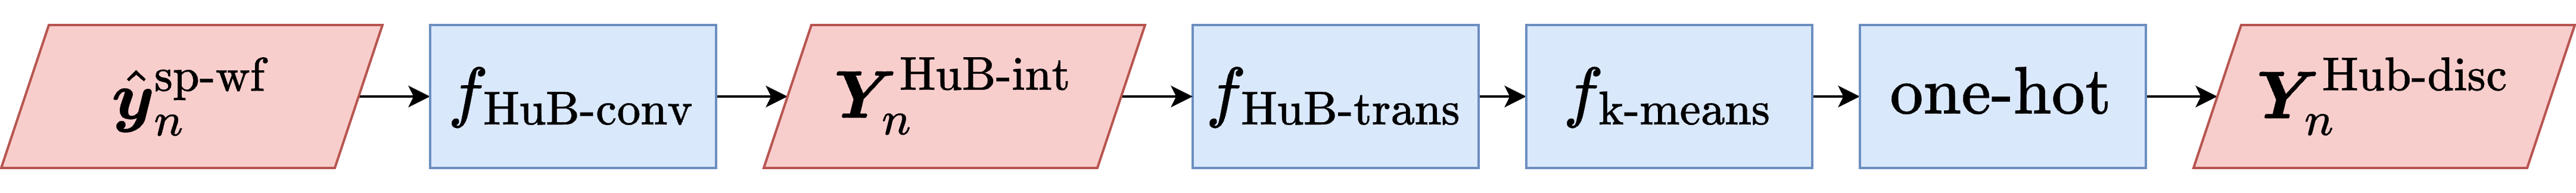
\includegraphics[height=12mm]{./figure/sec4/model_2/hubert.drawio.png}
    \caption{HuBERTを利用した特徴量計算の流れ}
    \label{sec4:fig:hubert}
\end{figure}

提案手法を図\ref{sec4:fig:overview}に示す.提案手法は,ネットワークA,ネットワークB,ボコーダの3つからなる.まず,ネットワークAを$\myNetworkA$とすると,$\myNetworkA$の行う処理は,
\begin{equation}
    \label{sec4:eq:networkA_overview}
    \hubertIntPred, \melPredA, \hubertDiscPredA = \myNetworkA\lr{\video, \spkEmb; \weightA}
\end{equation}
と表される.ここで,$\hubertIntPred \in \hubertIntSet$は予測HuBERT中間特徴量,$\melPredA \in \melSet$はネットワークAの予測メルスペクトログラム,$\hubertDiscPredA \in \hubertDiscPredSet$はネットワークAのHuBERT離散特徴量に対するロジットを表す.次に,ネットワークBを$\myNetworkB$とすると,$\myNetworkB$の行う処理は,
\begin{equation}
    \melPredB, \hubertDiscPredB = \myNetworkB\lr{\hubertIntPred, \spkEmb; \weightB}
\end{equation}
と表される.ここで,$\melPredB \in \melSet$はネットワークBの予測メルスペクトログラム,$\hubertDiscPredB \in \hubertDiscPredSet$はネットワークBのHuBERT離散特徴量に対するロジットを表す.最後に,音声波形を生成するボコーダを$\vocoder$とすると,$\vocoder$の行う処理は,
\begin{equation}
    \spWaveformPred = \vocoder\lr{\melPredB, \hubertDiscPredB; \weightVoc}
\end{equation}
と表される.まとめると,提案手法は口唇動画と話者ベクトルを入力とし,ネットワークAとネットワークBによって中間表現を獲得後,中間表現をボコーダに入力することで音声波形を生成するものである.

\begin{figure}[bt]
    \centering
    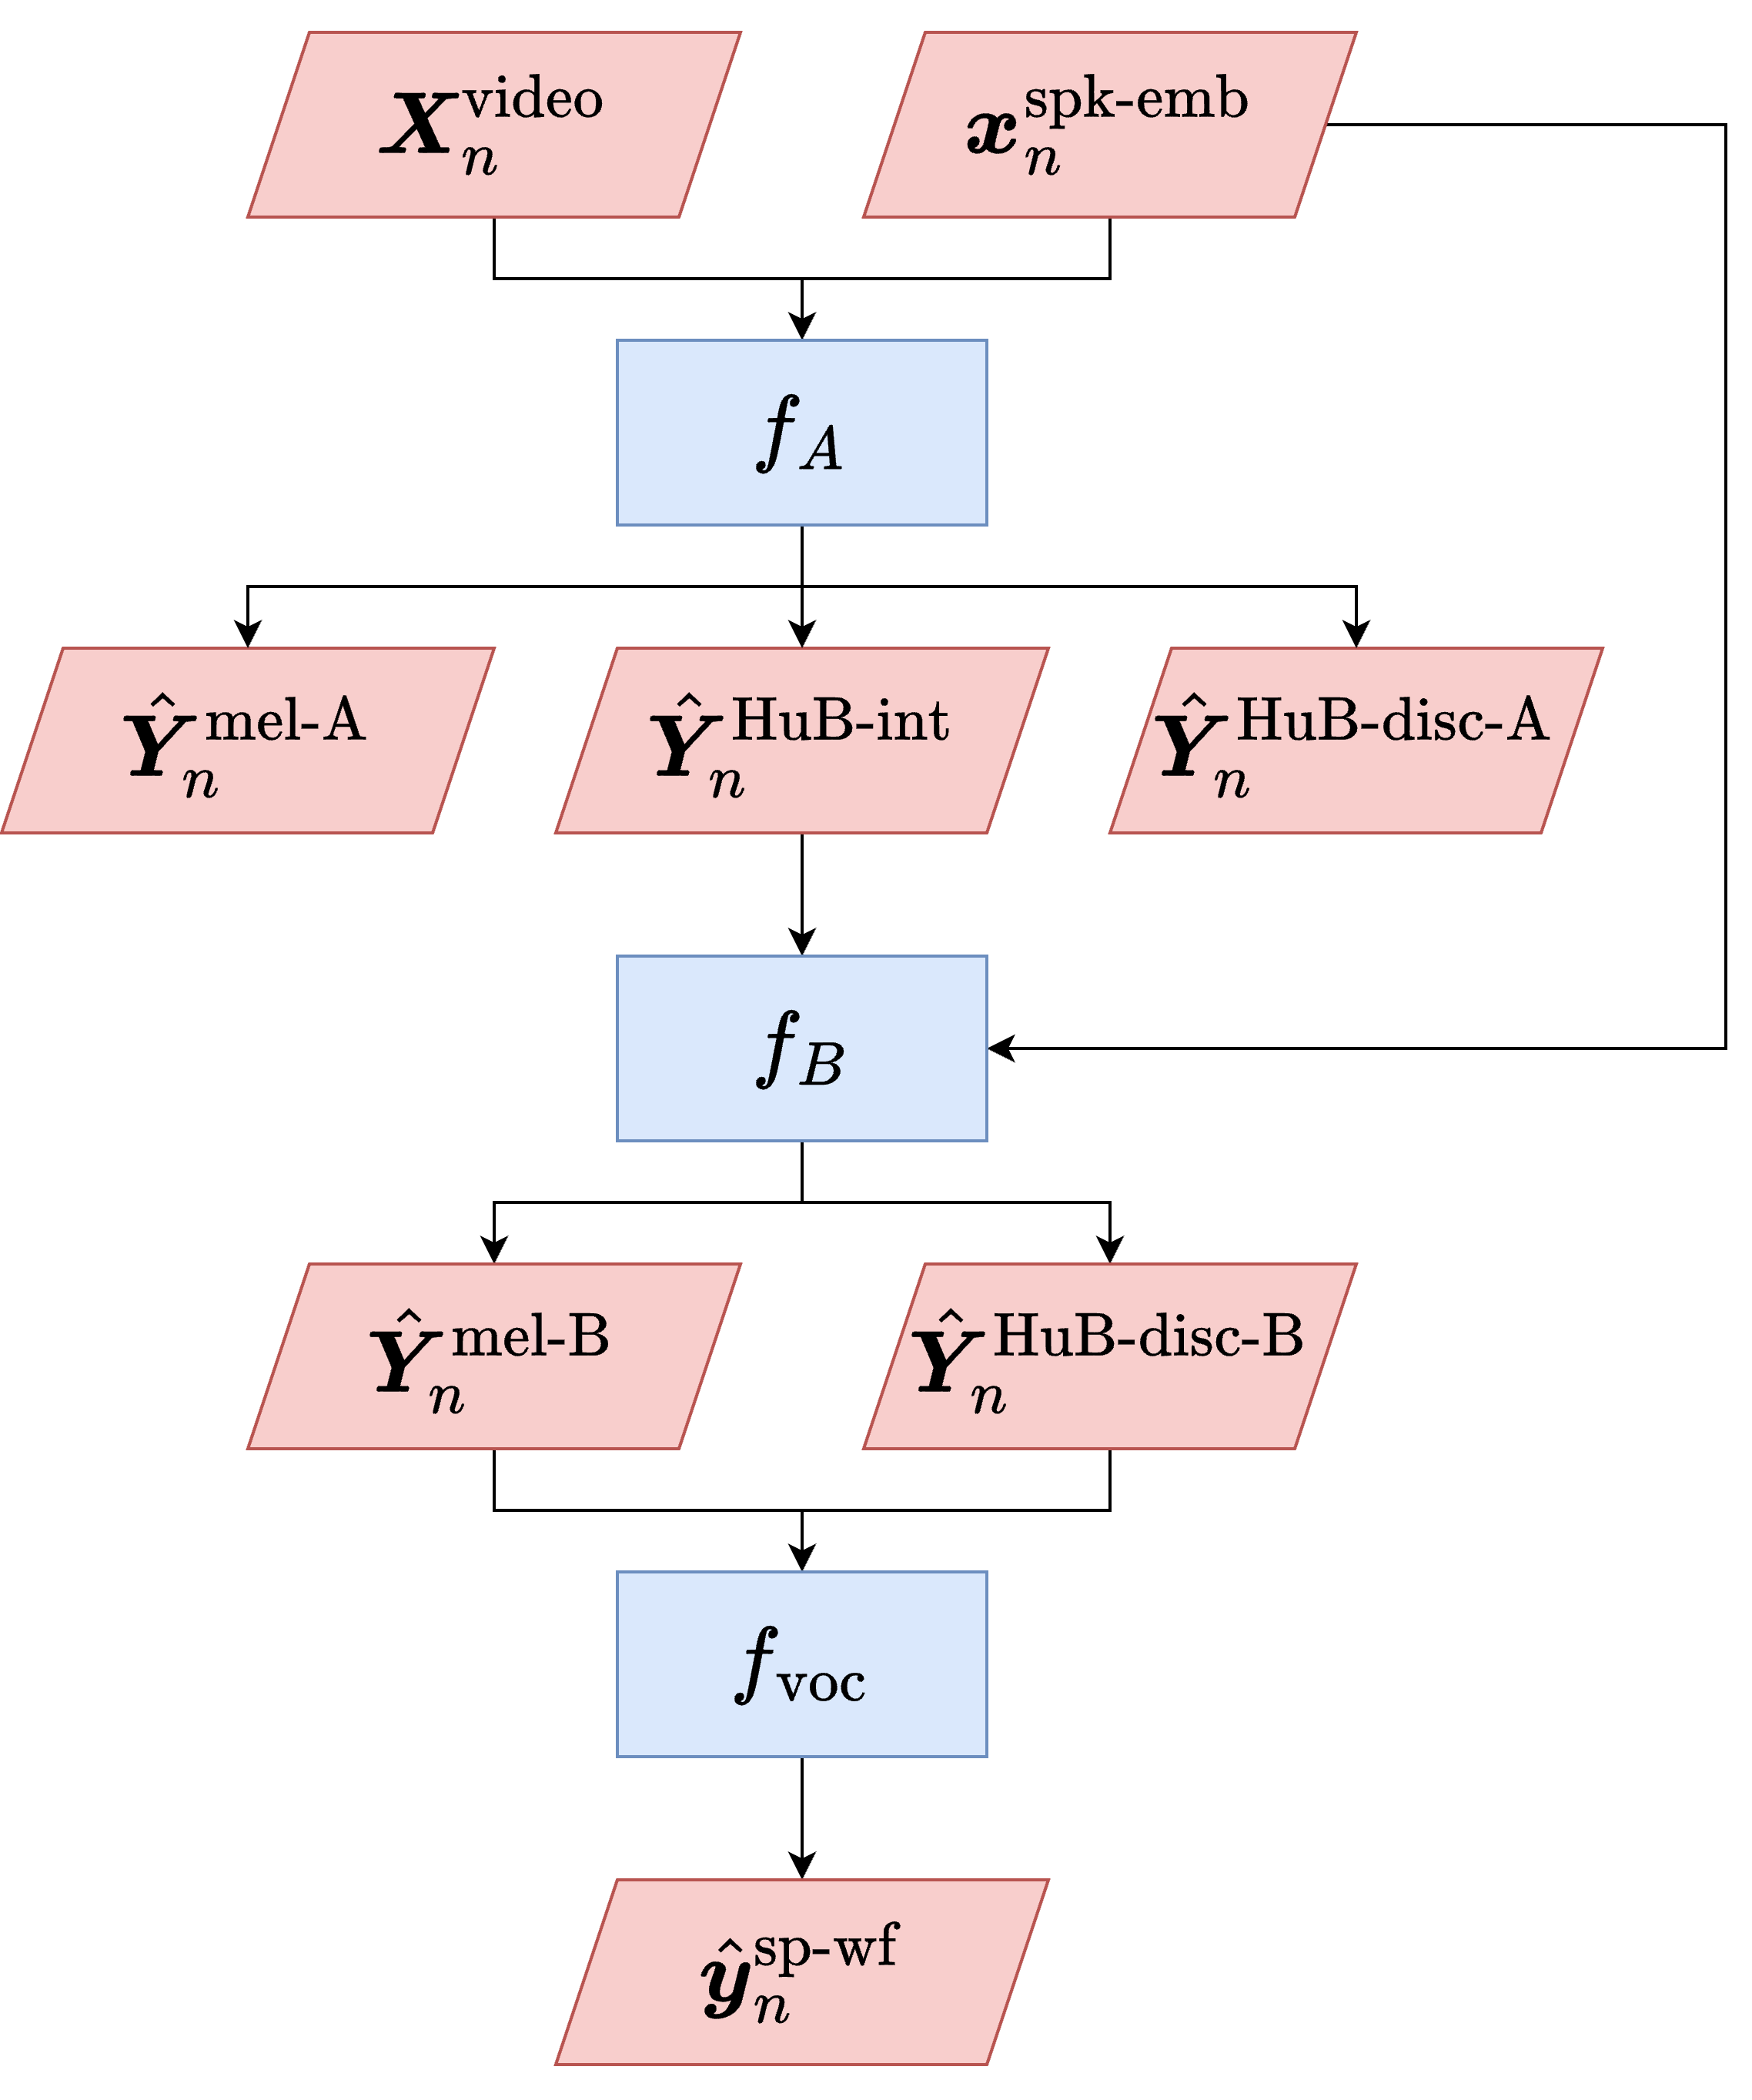
\includegraphics[height=100mm]{./figure/sec4/model_2/overview.drawio.png}
    \caption{提案手法の全体像}
    \label{sec4:fig:overview}
\end{figure}

\subsubsection{ネットワークA}
ネットワークAを図\ref{sec4:fig:networkA}に示す。ネットワークAでは,まず,口唇動画$\video$をAVHuBERTに通すことで,特徴量$\featureA \in \featureASet$に変換する.これは,
\begin{equation}
    \featureA = \AVHuBERT\lr{\video; \weightAAVHuBERT}
\end{equation}
と表される.$\weightAAVHuBERT$は,AVHuBERTの事前学習済み重みで初期化した.次に,$\featureA$の各時刻$t$におけるベクトルに対し,話者ベクトル$\spkEmb$を次元方向に結合してから,全結合層によって次元を再度圧縮し,元の次元に戻す.これは,
\begin{equation}
    \featureA = \myNetworkSpkMerge\lr{\concat{\featureA, \lrRepeat{\spkEmb}{T}}; \weightAFcSpk}
\end{equation}
と表される.次に,話者ベクトルが統合された特徴量に対する後処理として,$\myNetworkPost$を適用する.これは,
\begin{equation}
    \featureA = \myNetworkPost\lr{\featureA; \weightAPost}
\end{equation}
と表される.ここで、後処理層$\myNetworkPost$の構造を図\ref{sec4:fig:post_three_step}に示す。$\myNetworkPost$は,一次元畳み込み層を主としたConvBlockおよび,これに残差結合を組み合わせたResBlockから構成される.$\myNetworkPost$は,話者ベクトル$\spkEmb$が次元方向に結合された特徴量$\featureA$に対する話者性を考慮した特徴量の変換を行うために導入した。$\AVHuBERT$はMasked Predictionによって事前学習されたモデルだから、動画の文脈的な構造を考慮するのに適していると考えられる一方で、音声合成に必要となる話者性は発話に依存しない、すなわち動画の文脈的な構造とは別の性質を持った情報だと考えたからである.最後に,$\featureA$を全結合層を通して変換することで,予測対象であるHuBERT中間特徴量,メルスペクトログラム,HuBERT離散特徴量に対するロジットを得る.これは,
\begin{gather}
    \hubertIntPred = \myNetworkFcHubInt\lr{\featureA; \weightAFcHubInt} \\
    \melPredA = \myNetworkFcMel\lr{\featureA; \weightAFcMel} \\
    \hubertDiscPredA = \myNetworkFcHubDisc\lr{\featureA; \weightAFcHuBDisc}
\end{gather}
と表される.$\weightAFcSpk, \weightAPost, \weightAFcHubInt, \weightAFcMel, \weightAFcHuBDisc$は,すべてランダムに初期化した.

ネットワークAの役割は,続くネットワークBの入力であるHuBERT中間特徴量を予測することである.これに対し,メルスペクトログラムとHuBERT離散特徴量の推定を同時に行った理由は,先行研究\cite{kim2023lip_multitask,choi2023intelligible}においてマルチタスク学習の有効性が確認されており、HuBERT中間特徴量の推定においても有効ではないかと考えたからである。

\begin{figure}[tb]
    \centering
    \begin{subfigure}[b]{0.48\textwidth}
        \centering
        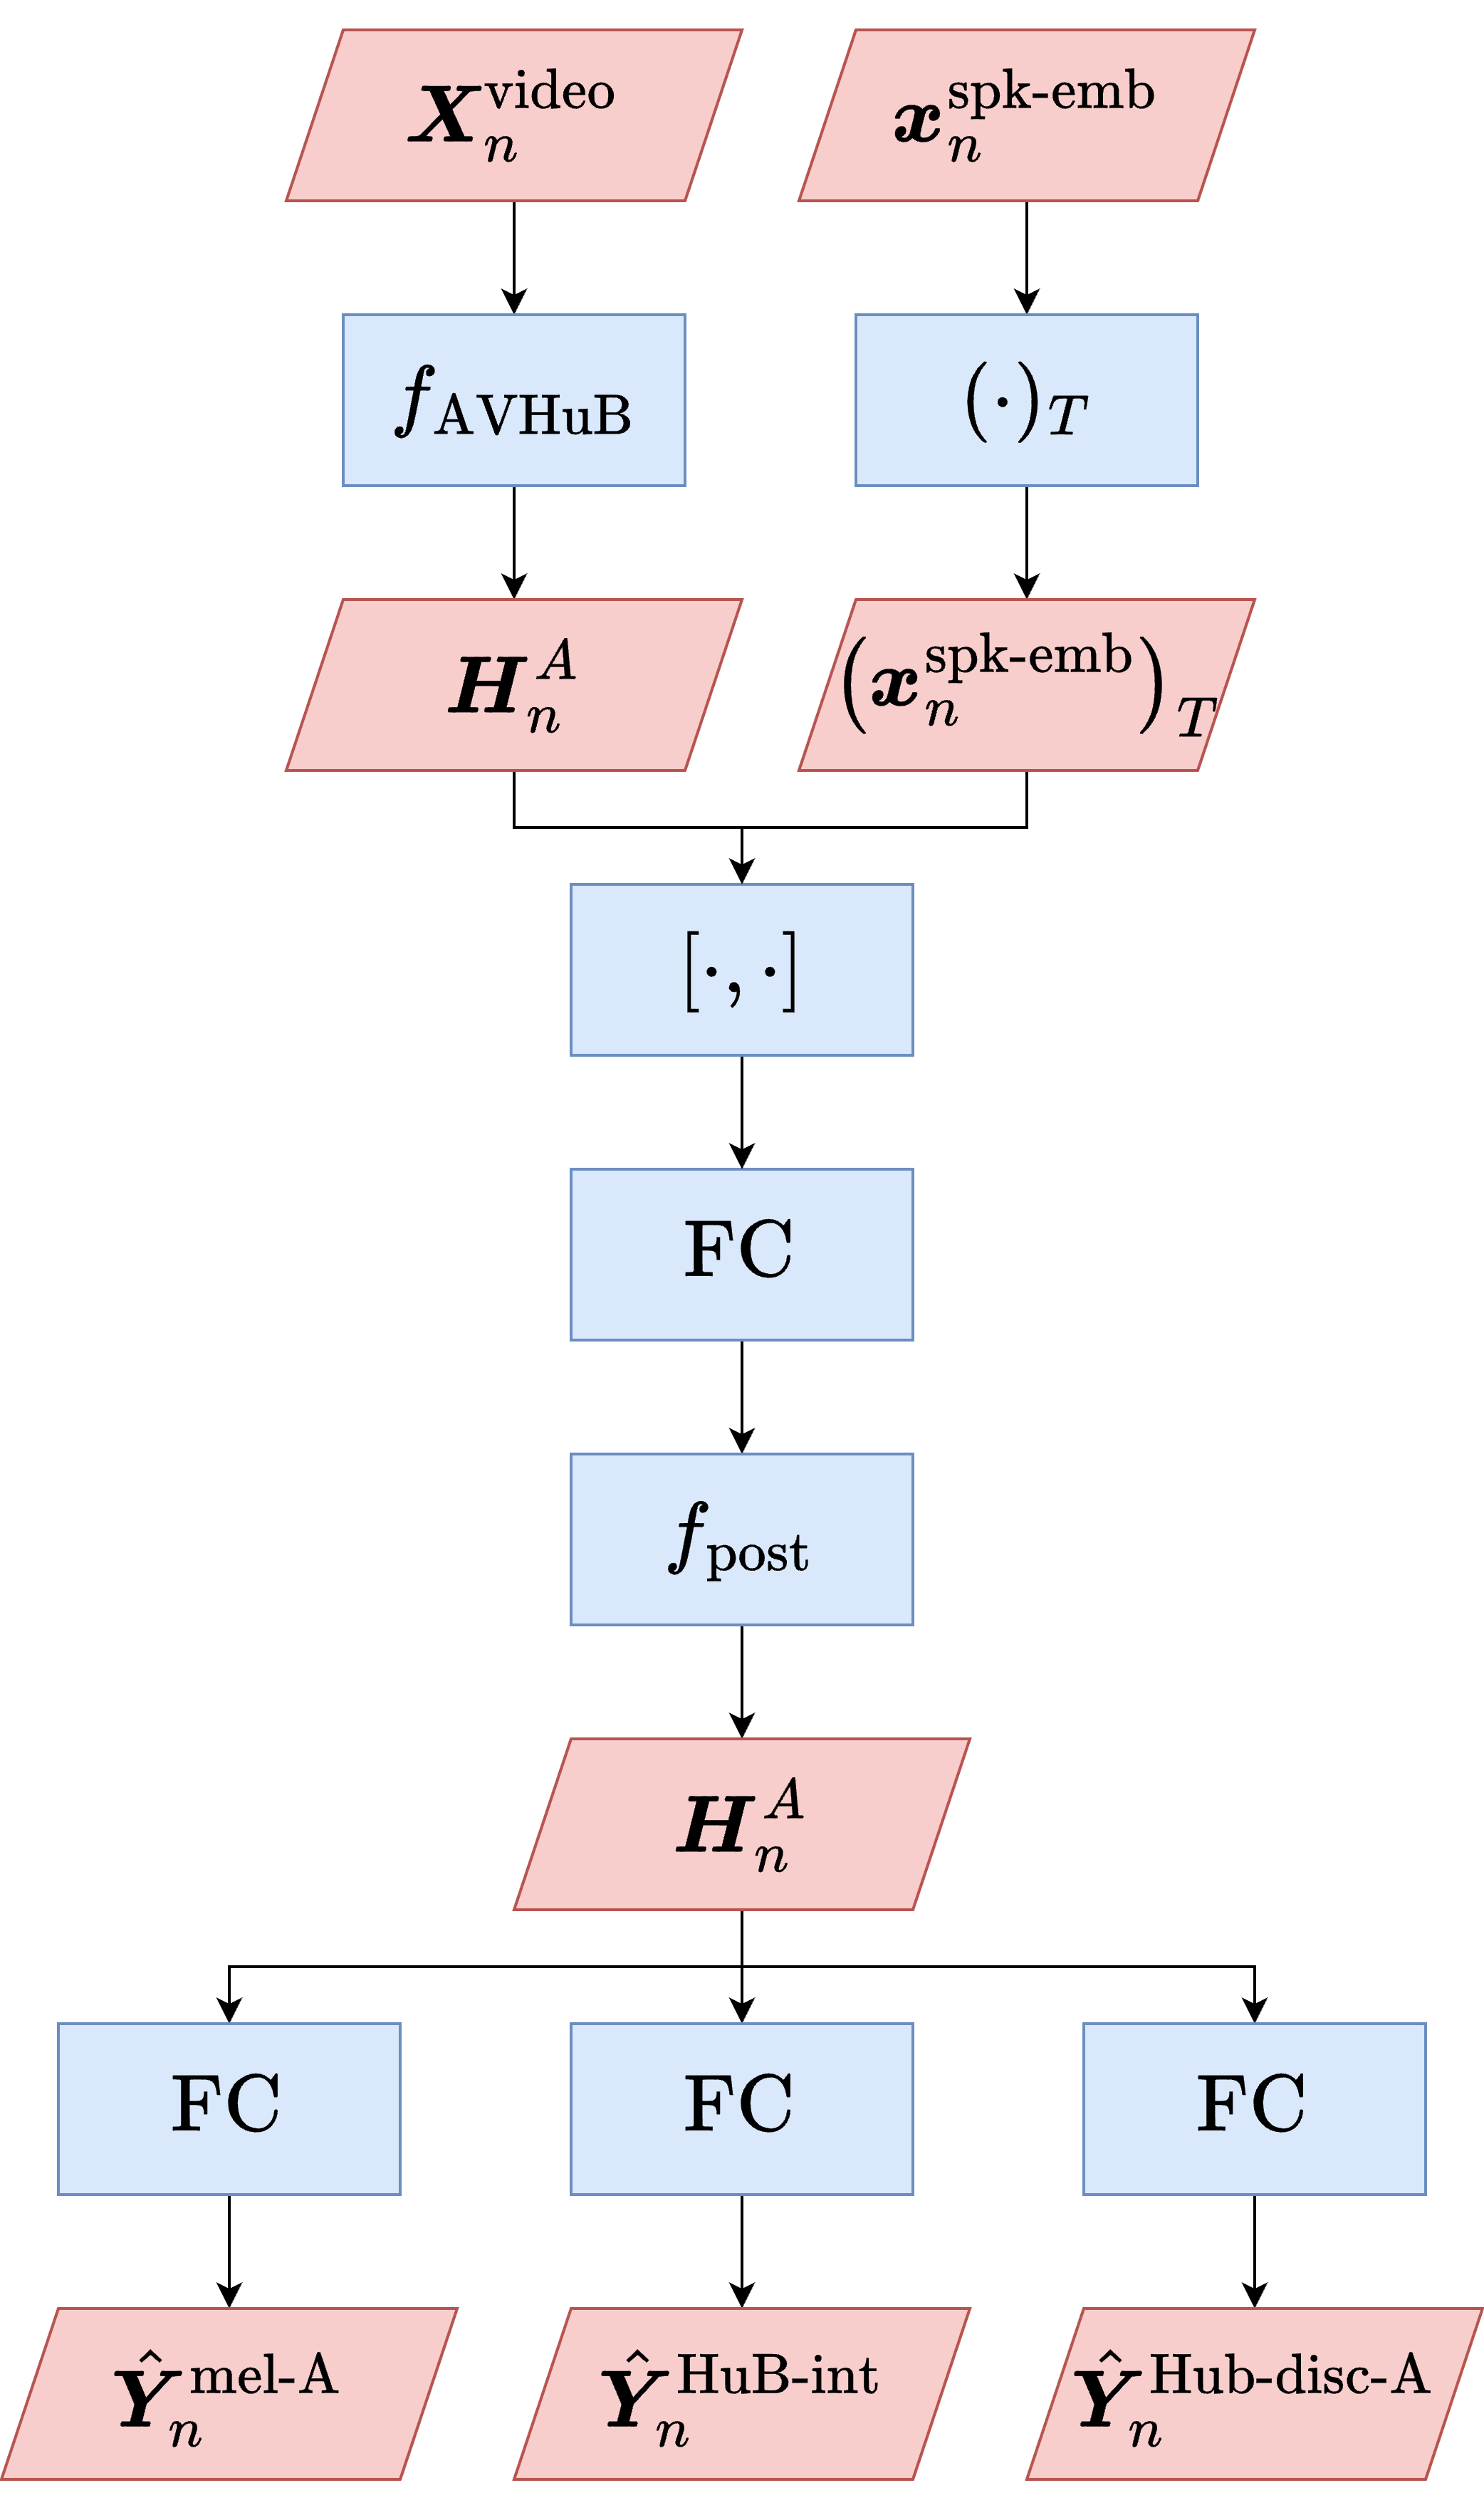
\includegraphics[height=120mm]{./figure/sec4/model_2/networkA.drawio.png}
        \caption{ネットワークA}
        \label{sec4:fig:networkA}
    \end{subfigure}
    \hfill
    \begin{subfigure}[b]{0.48\textwidth}
        \centering
        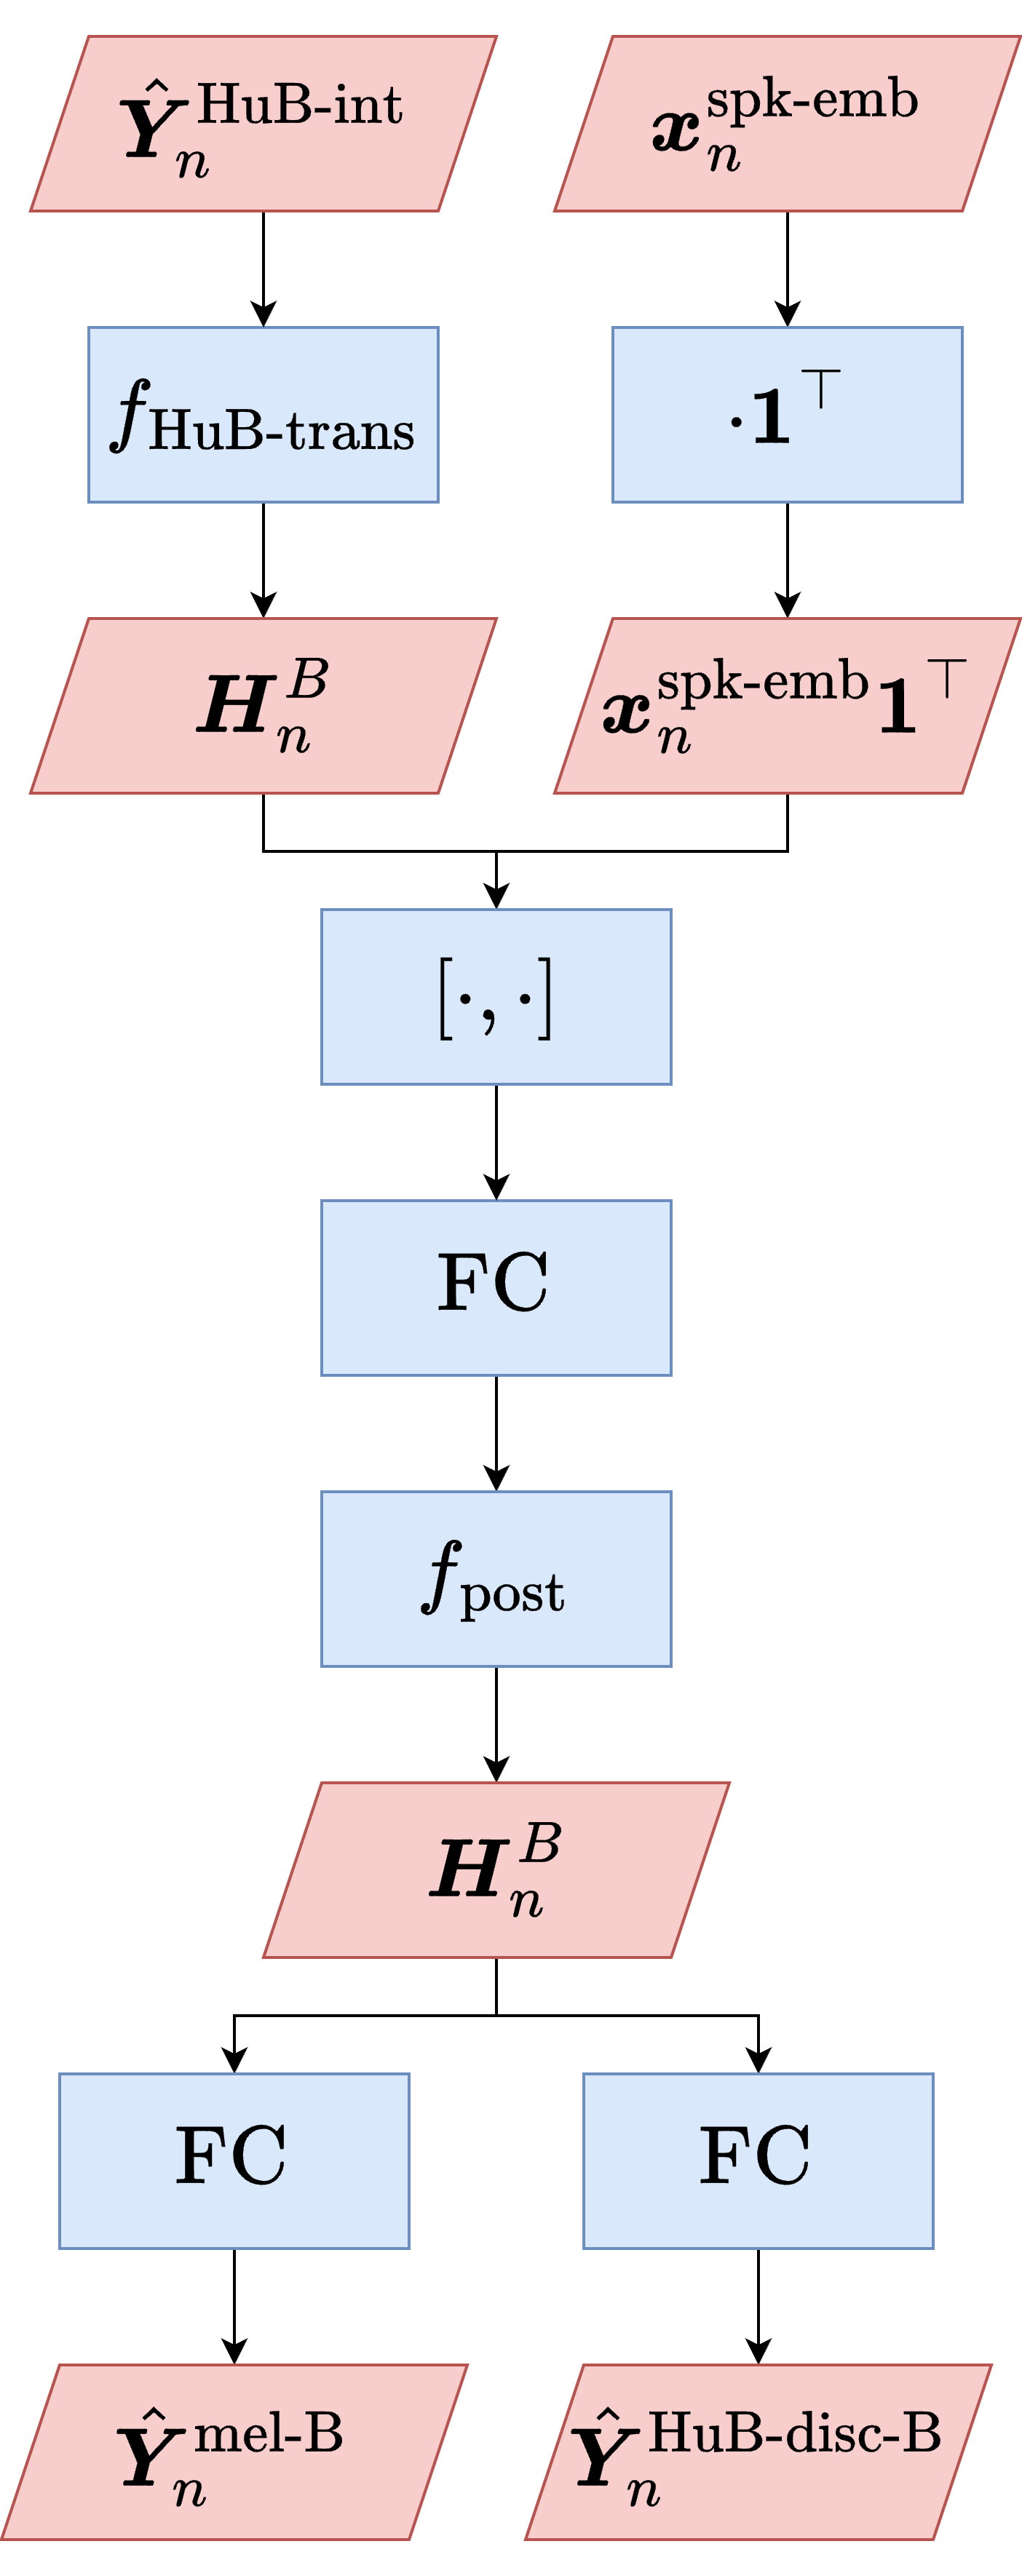
\includegraphics[height=120mm]{./figure/sec4/model_2/networkB.drawio.png}
        \caption{ネットワークB}
        \label{sec4:fig:networkB}
    \end{subfigure}
    \hfill
    \caption{ネットワークAとネットワークBの構造}
    \label{sec4:fig:networkAB}
\end{figure}

\begin{figure}[tb]
    \centering
    \begin{subfigure}[b]{0.32\textwidth}
        \centering
        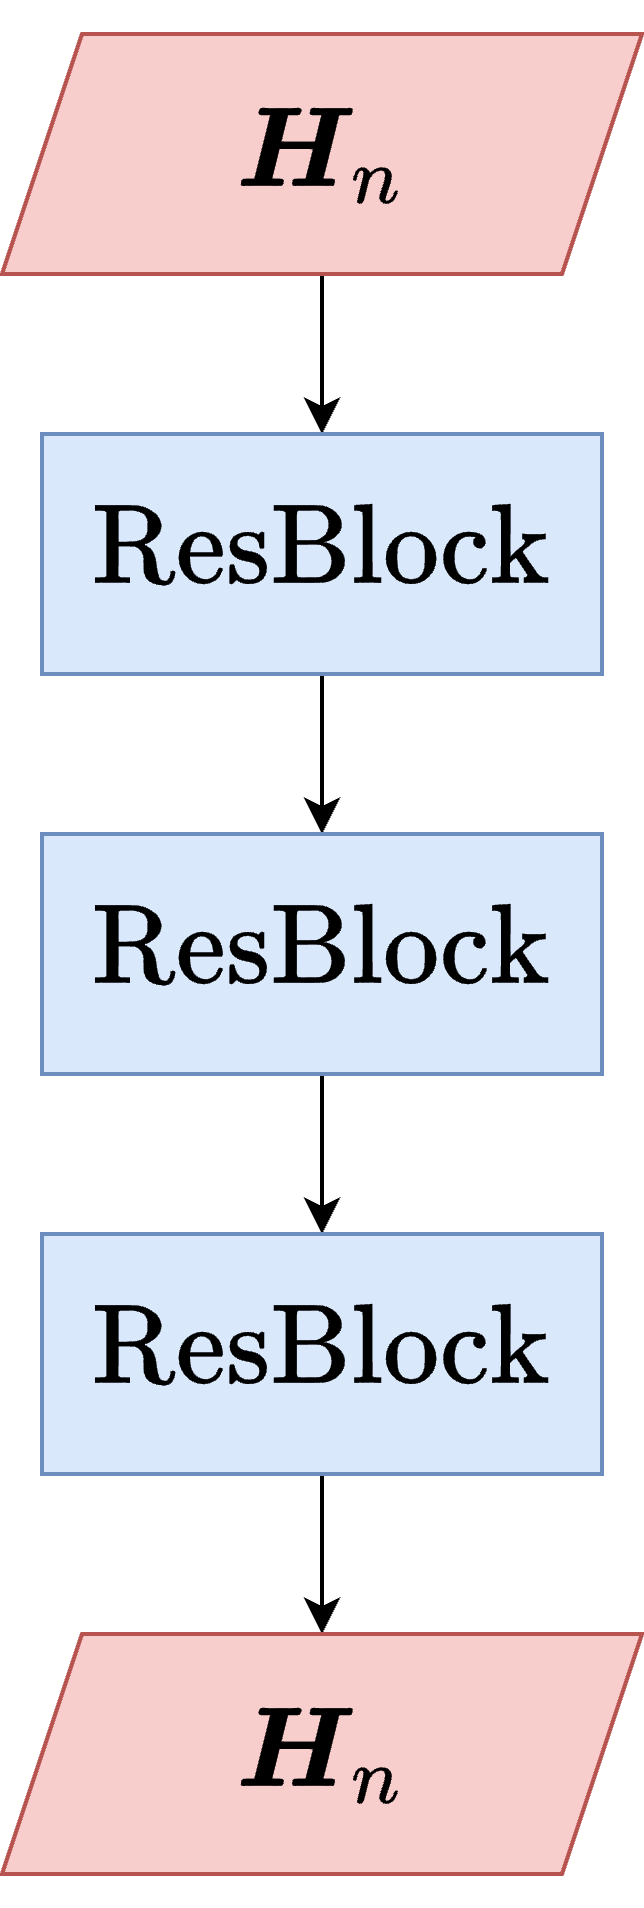
\includegraphics[height=70mm]{./figure/sec4/model_2/post.drawio.png}
        \caption{全体}
        \label{sec4:fig:post}
    \end{subfigure}
    \hfill
    \begin{subfigure}[b]{0.32\textwidth}
        \centering
        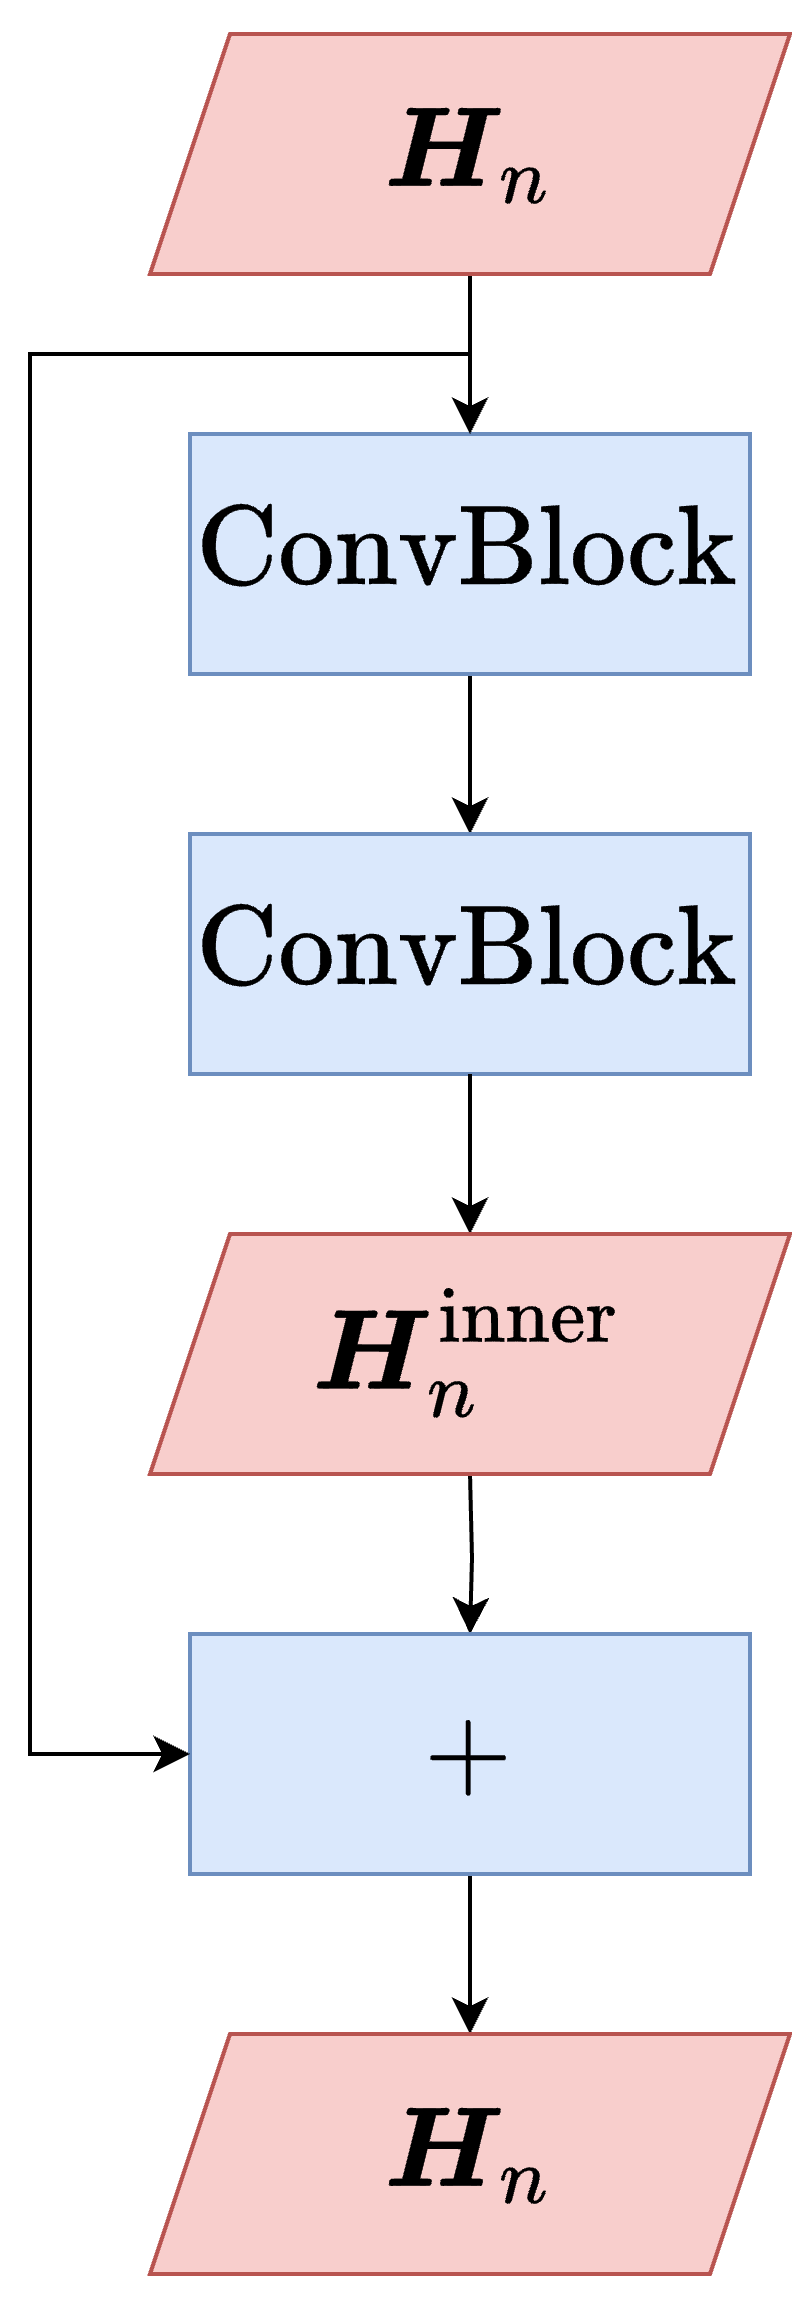
\includegraphics[height=70mm]{./figure/sec4/model_2/post_resblock.drawio.png}
        \caption{$\text{ResBlock}$}
        \label{sec4:fig:post_resblock}
    \end{subfigure}
    \hfill
    \begin{subfigure}[b]{0.32\textwidth}
        \centering
        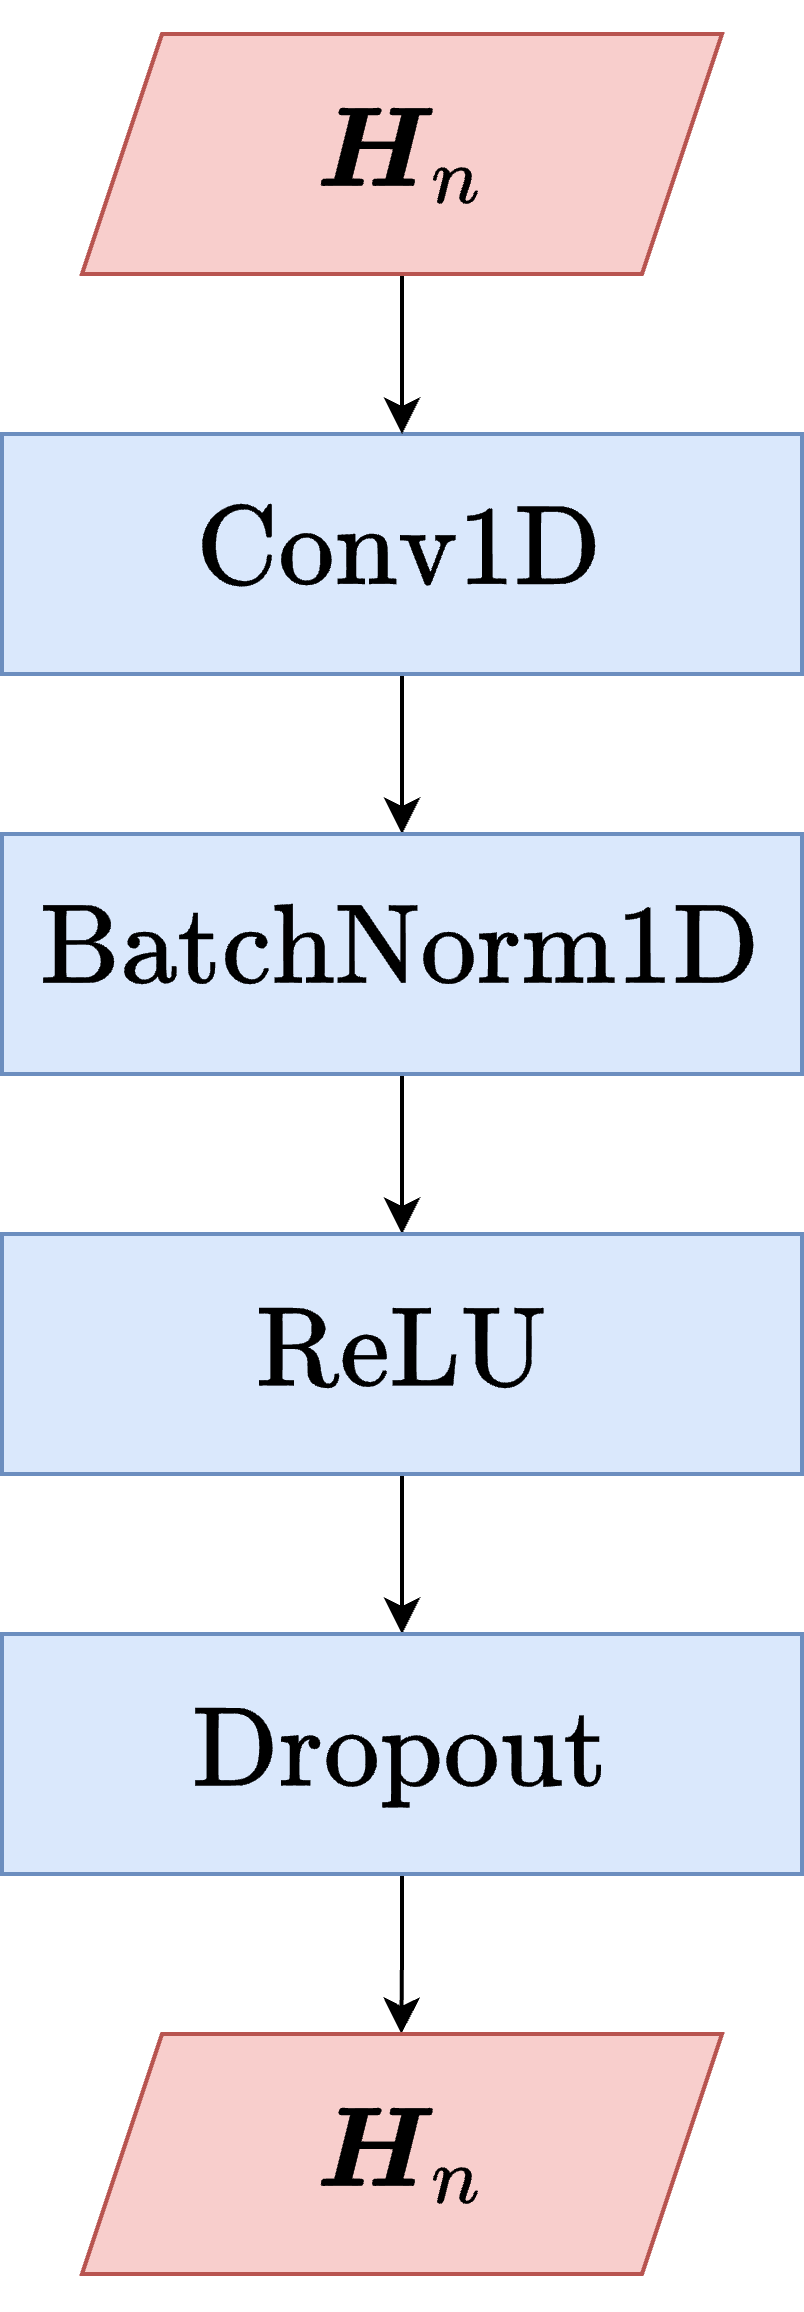
\includegraphics[height=70mm]{./figure/sec4/model_2/post_convblock.drawio.png}
        \caption{$\text{ConvBlock}$}
        \label{sec4:fig:post_convblock}
    \end{subfigure}
    \caption{後処理層$\myNetworkPost$の構造}
    \label{sec4:fig:post_three_step}
\end{figure}

\subsubsection{ネットワークB}
ネットワークBを図\ref{sec4:fig:networkB}に示す。ネットワークBでは,まず,ネットワークAで得られた予測HuBERT中間特徴量$\hubertIntPred$を$\hubertTransformer$に通すことで,特徴量$\featureB \in \featureBSet$に変換する.これは,
\begin{equation}
    \featureB = \hubertTransformer\lr{\hubertIntPred; \weightBHuBERTTrans}
\end{equation}
と表される.$\weightBHuBERTTrans$は,HuBERTの事前学習済み重みで初期化する場合と,ランダム初期化する場合の2つを検討した.以下,ネットワークAと処理は同様であるため,数式のみ記載する.
\begin{gather}
    \featureB = \myNetworkSpkMerge\lr{\concat{\featureB, \lrRepeat{\spkEmb}{T}}; \weightBFcSpk} \\
    \featureB = \myNetworkPost\lr{\featureB; \weightBPost} \\
    \melPredB = \myNetworkFcMel\lr{\featureB; \weightBFcMel} \\
    \hubertDiscPredB = \myNetworkFcHubDisc\lr{\featureB; \weightBFcHuBDisc}
\end{gather}
$\weightBFcSpk, \weightBPost, \weightBFcMel, \weightBFcHuBDisc$は,すべてランダムに初期化した.

ネットワークBの役割は,メルスペクトログラムとHuBERT離散特徴量の予測である.HuBERT Transformer層の転移学習を検討した狙いは、HuBERTの自己教師あり学習の方法に基づく。HuBERTはMasked Predictionという自己教師あり学習を行っており、これは、畳み込みエンコーダ$\hubertConv$からの出力にマスクを適用し,Transformer層$\hubertTransformer$を通すことによって、マスクされたフレームにおける教師ラベルを推定する学習方法である.\ref{sec3:sec:ssl}節より、Masked Predictionでは欠損された入力から特徴抽出を行う必要があるから,最適化されたHuBERTは音声の文脈的な構造を学習していると考えられる.また、Masked Predictionは音声データのみによる学習が可能であり、近年では大規模なデータによって学習されたモデルも一般に公開されている。よって、本研究ではHuBERT Transformer層を動画音声合成にFine Tuningすることにより,動画を入力とするネットワークAの推定残差を,大量の音声データから学習された音声自体の文脈を考慮する力によって軽減することで、最終予測値であるメルスペクトログラムとHuBERT離散特徴量に対する推定精度改善を狙った.

\subsubsection{ボコーダ}
ボコーダを図\ref{sec4:fig:vocoder}に示す。本実験で用いるボコーダは、今回ベースラインとする先行研究\cite{choi2023intelligible}で提案されたMulti-input Vocoderを参考にしたものである。まず,ネットワークBで得られた予測メルスペクトログラム$\melPredB$とHuBERT離散特徴量に対するロジット$\hubertDiscPredB$を前処理層に通し,扱いやすい形状に変換する.これは,
\begin{gather}
    \featureVocMel = \vocoderPreMel\lr{\melPredB; \weightVocPreMel} \\
    \featureVocHuBERT = \vocoderPreHub\lr{\hubertDiscPredB; \weightVocPreHuB}
\end{gather}
と表される.$\featureVocMel \in \featureVocMelSet$は,$\melPredB$の時間方向に隣接したベクトルを次元方向に結合することで$\hubertDiscPredB$と系列長を揃え、その後全結合層を適用した特徴量である.一方,$\featureVocHuBERT \in \featureVocHuBERTSet$は,$\hubertDiscPredB$に対して$\argmax$関数を適用した後,各時刻$t$において選択されたインデックスをベクトルに変換した特徴量である.次に,$\featureVocMel, \featureVocHuBERT$を入力として,音声波形を生成する.これは,
\begin{equation}
    \spWaveformPred = \vocoderMain\lr{\concat{\featureVocMel, \featureVocHuBERT}; \weightVocMain}
\end{equation}
と表される.$\vocoderMain$は,図\ref{sec4:fig:vocoder_main}に示すように,一次元畳み込み層とUpsamplingBlockから構成され,これはHiFi-GANのGeneratorと同様である.各UpsamplingBlockでは,初めに一次元転置畳み込み層を通すことで時間方向のアップサンプリングを行い,その後複数の一次元畳み込み層から特徴抽出を行った結果を平均して出力する.

\begin{figure}[tb]
    \centering
    \begin{subfigure}[b]{0.32\textwidth}
        \centering
        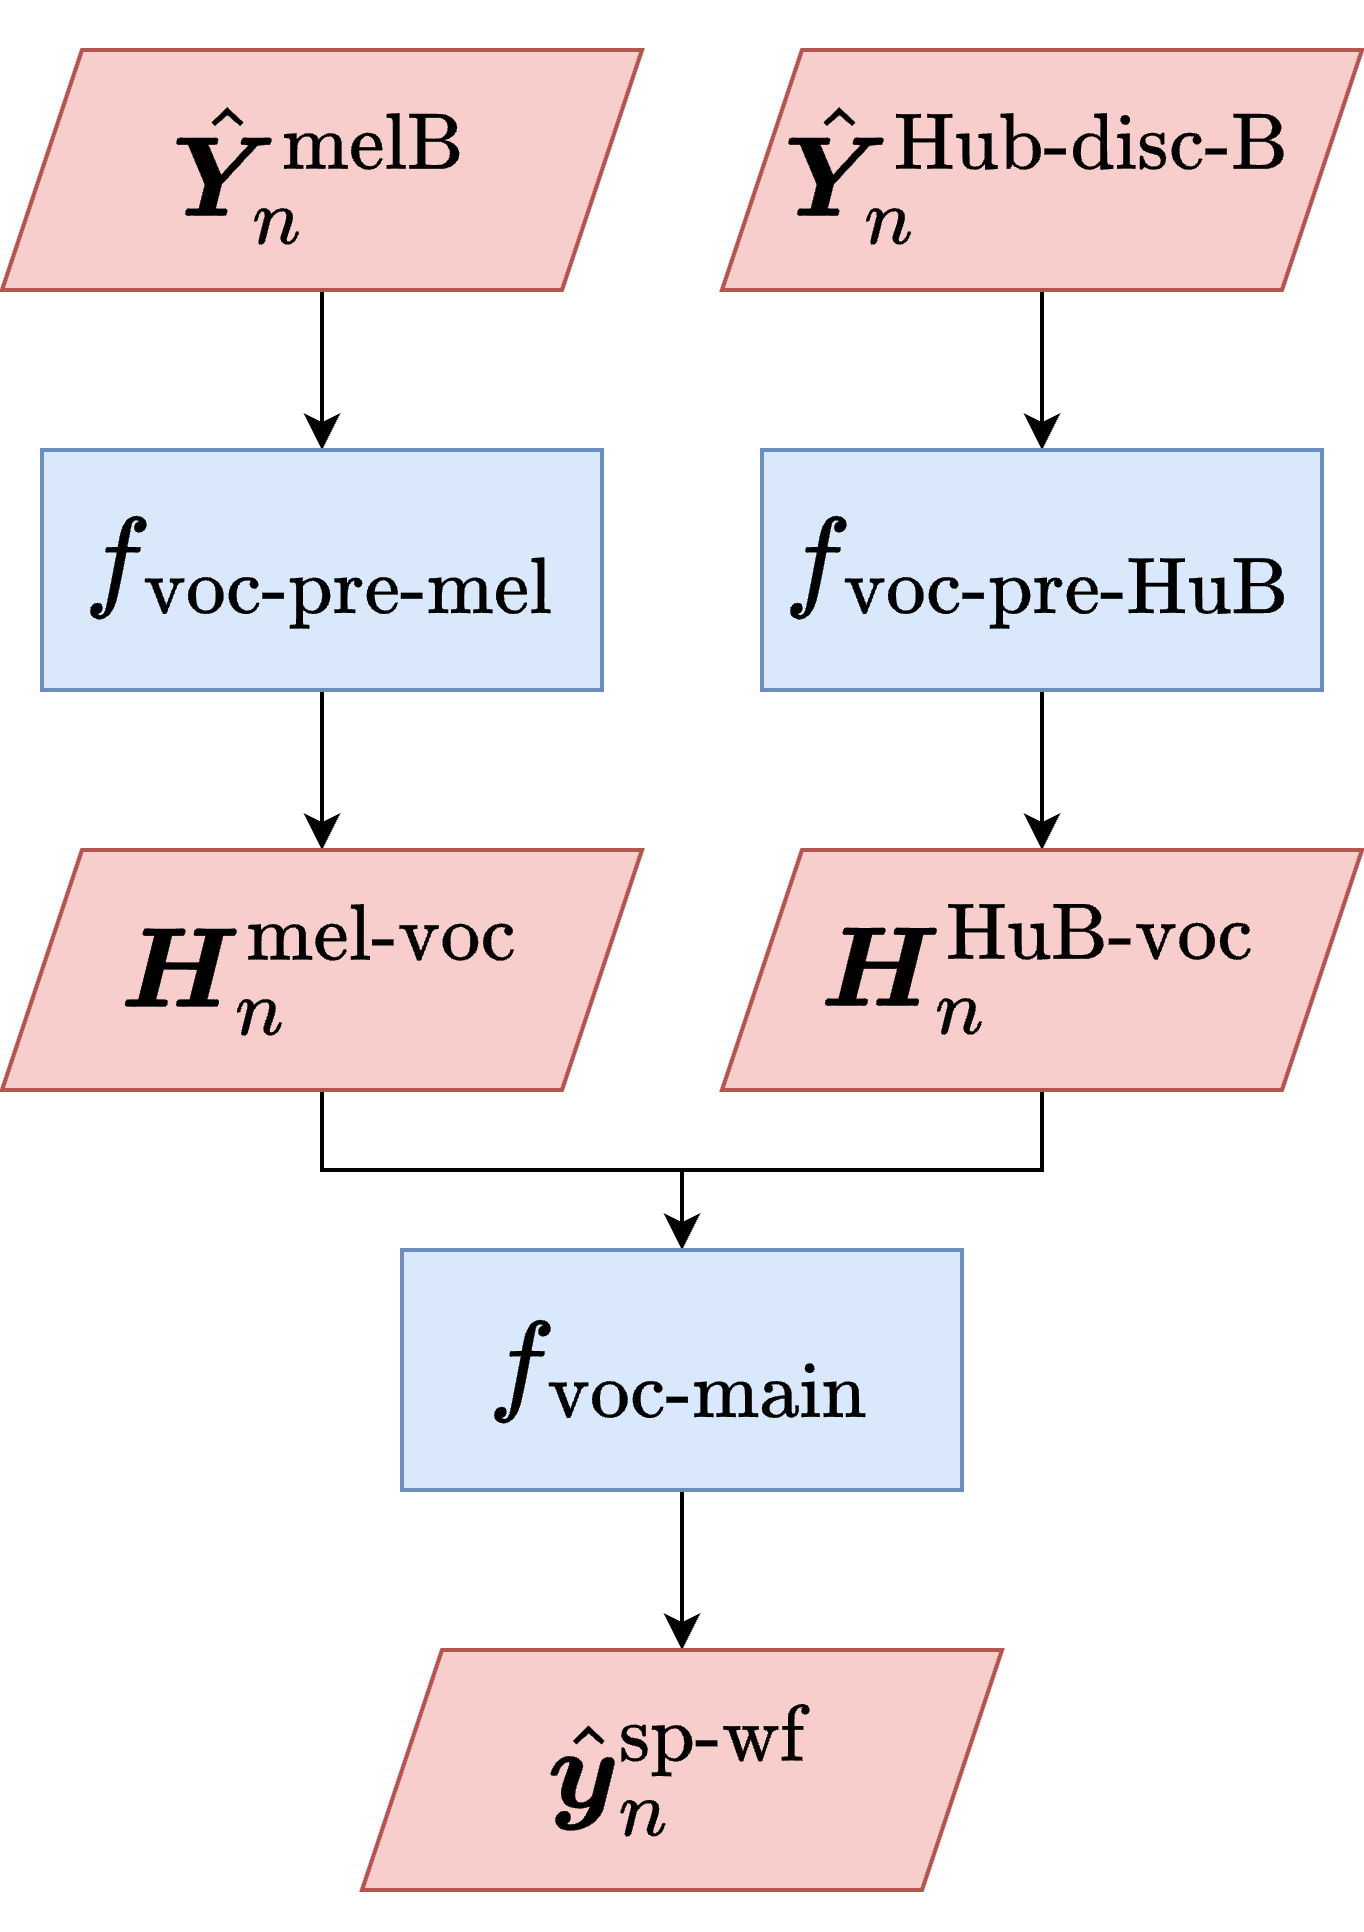
\includegraphics[width=45mm]{./figure/sec4/model_2/vocoder.drawio.png}
        \caption{全体}
        \label{sec4:fig:vocoder_overview}
    \end{subfigure}
    \hfill
    \begin{subfigure}[b]{0.32\textwidth}
        \centering
        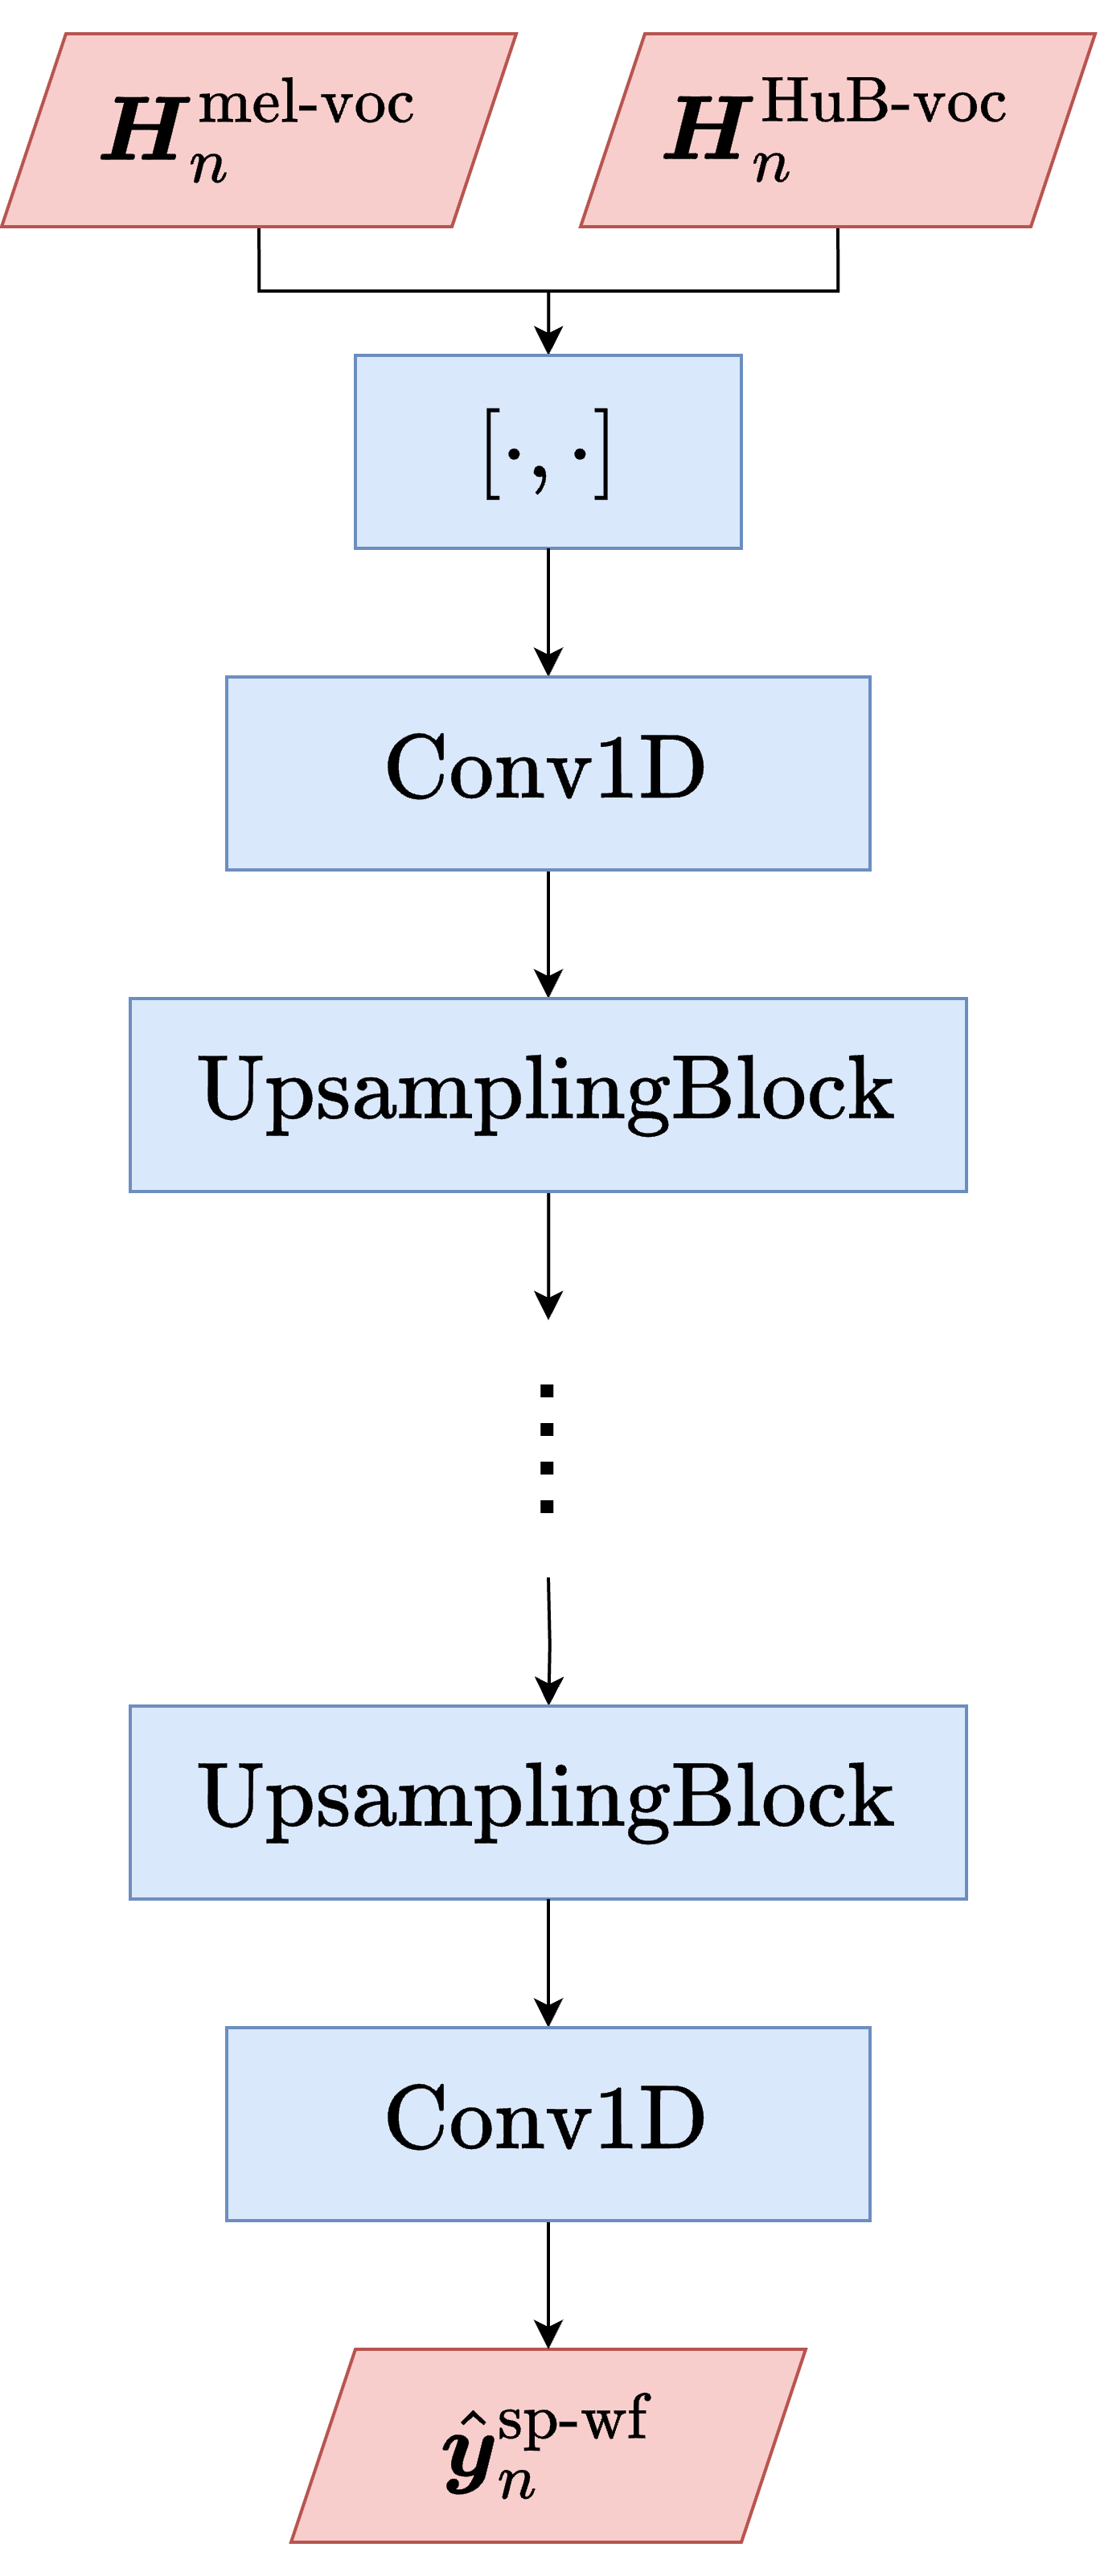
\includegraphics[width=45mm]{./figure/sec4/model_2/vocoder_main.drawio.png}
        \caption{$\vocoderMain$}
        \label{sec4:fig:vocoder_main}
    \end{subfigure}
    \hfill
    \begin{subfigure}[b]{0.32\textwidth}
        \centering
        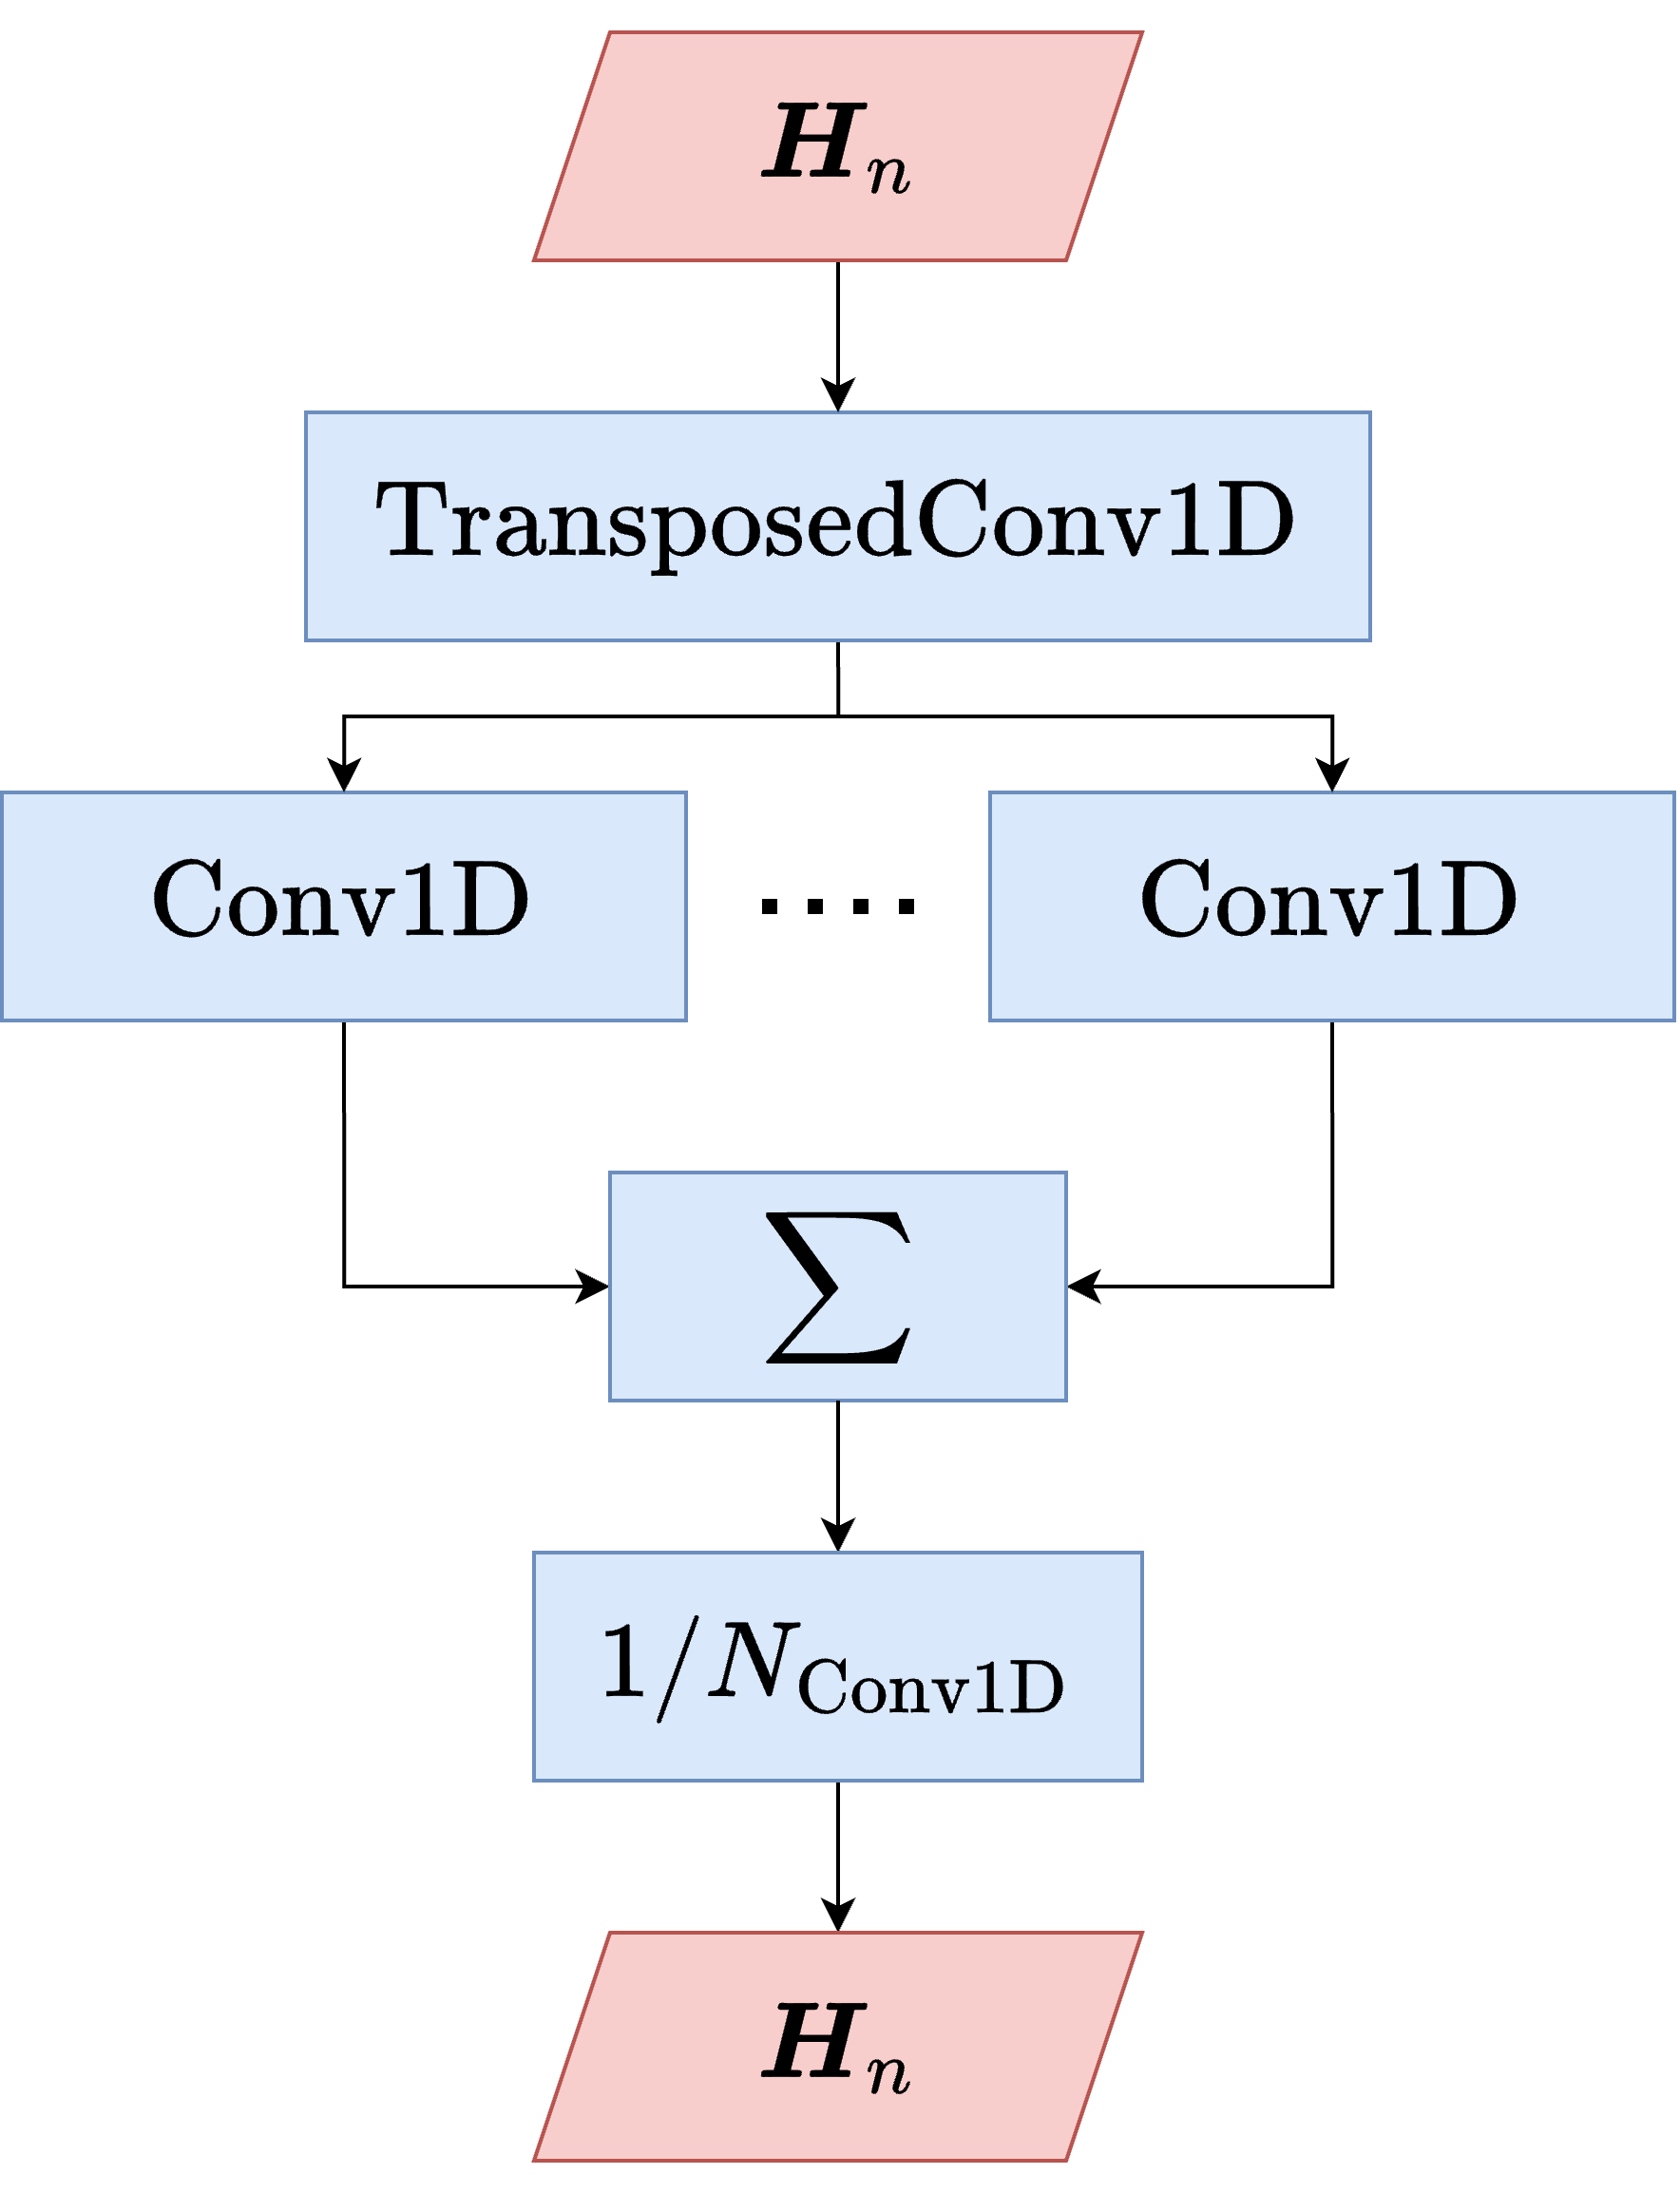
\includegraphics[width=45mm]{./figure/sec4/model_2/vocoder_main_block.drawio.png}
        \caption{$\text{UpsamplingBlock}$}
        \label{sec4:fig:vocoder_main_block}
    \end{subfigure}
    \caption{ボコーダの構造}
    \label{sec4:fig:vocoder}
\end{figure}

\subsubsection{損失関数}
まず,ネットワークAの学習に用いる損失関数$\lossA$は,
\begin{equation}
    \begin{aligned}
        \lossA & \lr{\hubertIntGt, \hubertIntPred, \melGt, \melPredA, \hubertDiscGt, \hubertDiscPredA}                 \\
        =      & \lossWeightHubInt \lossMAE{\hubertIntGt}{\hubertIntPred} + \lossWeightMel \lossMAE{\melGt}{\melPredA} \\
               & + \lossWeightHubDisc \lossCE{\hubertDiscGt}{\hubertDiscPredA}
    \end{aligned}
\end{equation}
で与えられる.すなわち,HuBERT中間特徴量についてのMAE Loss,メルスペクトログラムについてのMAE Loss,HuBERT離散特徴量についてのCross Entropy Lossの重み付け和である.次に,ネットワークBの学習に用いる損失関数$\lossB$は,
\begin{equation}
    \begin{aligned}
        \lossB & \lr{\melGt, \melPredB, \hubertDiscGt, \hubertDiscPredB}                                                  \\
        =      & \lossWeightMel \lossMAE{\melGt}{\melPredB} + \lossWeightHubDisc \lossCE{\hubertDiscGt}{\hubertDiscPredB}
    \end{aligned}
\end{equation}
で与えられる.すなわち,メルスペクトログラムについてのMAE Loss,HuBERT離散特徴量についてのCross Entropy Lossの重み付け和である.最後に,ボコーダの学習に用いる損失関数について,これはHiFi-GANと同様であるから,ここでは割愛する.

\subsection{実験方法}
\subsubsection{利用したデータセット}
動画音声データセットには,先行研究\cite{taguchi,esaki}で収録されたもののうち,ATR音素バランス文\cite{atr}を読み上げたデータを利用した.このデータセットは、男女二人ずつから収録された合計4人分のデータから構成される。分割は,AからHセットを学習データ,Iセットを検証データ,Jセットをテストデータとした.各分割ごとの文章数を表~\ref{sec4:tab:dataset_info}に示す.

ボコーダの学習には,Hi-Fi-Captain\cite{okamoto2023hi}とJVS\cite{takamichi2019jvs}を利用した.Hi-Fi-Captainは,日本語話者2名と英語話者2名からなるデータセットであるが,本実験では日本語話者2名分のデータのみを利用した.分割は,train-parallelおよびtrain-non-parallelを学習データ,valを検証データ,evalをテストデータとした.各分割ごとの文章数を表~\ref{sec4:tab:dataset_info}に示す.JVSは100人の日本語話者からなるデータであり,各話者に対して1から100まで番号が割り振られている.読み上げ音声のparallel100およびnonpara30と,裏声のfalset10,囁き声のwhisper10が含まれるが,本研究ではparallel100とnonpara30のみ利用した.分割は,1から80番の話者を学習データ,81番から90番の話者を検証データ,91番から100番までの話者をテストデータとした.各分割ごとの文章数を表~\ref{sec4:tab:dataset_info}に示す.

\begin{table*}[bt]
    \centering
    \caption{利用したデータセットの文章数}
    \label{sec4:tab:dataset_info}
    \begin{center}
        \renewcommand{\arraystretch}{0.9} % 行の高さ調整
        \setlength{\tabcolsep}{8pt}      % 列の幅調整
        \scalebox{1.0}{
            \begin{tabular}{|l|r|r|r|}
                \hline
                              & \multicolumn{1}{c|}{学習} & \multicolumn{1}{c|}{検証} & \multicolumn{1}{c|}{テスト} \\
                \hline
                動画音声データセット    & 1598                    & 200                     & 212                      \\
                Hi-Fi-Captain & 37714                   & 200                     & 200                      \\
                JVS           & 10398                   & 1299                    & 1300                     \\
                \hline
            \end{tabular}
        }
    \end{center}
\end{table*}

\subsubsection{データの前処理}
動画データは60 FPSで収録されたものをffmpegにより25 FPSに変換して用いた.その後,手法\cite{bulat2017far}により動画に対してランドマーク検出を適用した\footnote{\url{https://github.com/1adrianb/face-alignment}}.このランドマークを利用することで口元のみを切り取り,画像サイズを$\lr{96, 96}$にリサイズした.モデル入力時は動画をグレースケールに変換し,各フレームに対する正規化および標準化を適用した.全体として,今回はAVHuBERTの転移学習を行うため,そこでの前処理に合わせている.学習時のデータ拡張は,ランダムクロップ,左右反転,Time Maskingを適用した.ランダムクロップは,$\lr{96, 96}$で与えられる画像から$\lr{88, 88}$をランダムに切り取る処理である.検証およびテスト時は,必ず画像中央を切り取るよう実装した.左右反転は,50\%の確率で左右が反転されるよう実装した.Time Maskingは,動画1秒あたり0から0.5秒の間でランダムに停止区間を定め,その区間における動画の時間方向平均値を計算し,区間内のすべてのフレームをこの平均値で置換した.これにより,動画が一時停止されるような効果が得られる.

音声データは16 kHzにダウンサンプリングして用いた.窓長25 msのハニング窓を用いてシフト幅10 msでSTFTを適用することで,フレームレート100 Hzのスペクトログラムに変換し,パワースペクトログラムに対して80次のメルフィルタバンクを適用した後,対数スケールに変換することで対数メルスペクトログラムを得た.また,Hi-Fi-CaptainとJVSには,ボコーダの学習安定化のため,無音区間のトリミング(-40 dBFS未満かつ500 ms継続する区間を100 msまでカット)を適用した.

モデルへの入力とした話者ベクトルは,動画音声データセット,Hi-Fi-Captain,JVSともに,各話者に対し学習データの中から100文章をランダムサンプリングし,各発話に対して得られたベクトルの平均値を用いた.これを学習・検証・テストで一貫して用いるため,検証データやテストデータには非依存な値となっている.

HuBERT離散特徴量の計算に利用するHuBERT Transformer層出力は,8層目出力を利用した.HuBERTの層ごとの特徴量について,音素のOne-hotベクトルおよび単語のOne-hotベクトルとの相関をCanonical Correlation Analysis(CCA)によって調べた先行研究\cite{pasad2023comparative}より,8層目出力がそのどちらとも相関が高いことが示されている.本実験では,HuBERT離散特徴量は言語的な情報を持つものとして扱いたかったため,この層からの出力を利用した.k-means法のクラスタ数は100とし,動画音声データセットの学習用データを利用して学習した後,全データセットに対してクラスタリングを実施した.また,学習時はゼロパディングされる区間のためにクラスを一つ追加したため,合計101クラスとして扱った.

\subsubsection{本実験で利用した事前学習済みモデルについて}
話者ベクトルの計算に用いた話者識別モデルの事前学習済み重みには,VoxCeleb1\cite{nagrani2020voxceleb}とVoxCeleb2,LibriSpeech\cite{panayotov2015librispeech}のotherセットで学習されたものを用いた\footnote{\url{https://github.com/resemble-ai/Resemblyzer}}.学習データセットの記述は,このモデルを利用して複数話者TTSを検討した先行研究\cite{jia2018transfer}のGitHubリポジトリにある\footnote{\url{https://github.com/CorentinJ/Real-Time-Voice-Cloning/wiki/Training}}.話者識別モデルは,音声波形をメルスペクトログラムに変換した後,これを1.6秒ごとに0.77秒のオーバーラップを持つよう分割し,各区間ごとに一つのベクトル表現を獲得した後,区間ごとの出力ベクトルを平均して正規化することで最終出力を得る.モデル構造は3層のLSTMと全結合層からなり,得られる話者ベクトルの次元は256次元である.

AVHuBERTの事前学習済み重みには,LRS3とVoxCeleb2の英語データを利用し,データ拡張として音声データにノイズを付与した場合\cite{shi2022robust}の重みを利用した\footnote{\url{https://github.com/facebookresearch/av_hubert}}.脚注のリンク先では,「Model: Noise-Augmented AV-HuBERT Base」,「Pretraining Data: LRS3 + VoxCeleb2 (En)」,「Finetuning Data: No finetuning」と示されている.ノイズ付与の場合を利用した理由は,音声にノイズが含まれることで動画からの特徴抽出が促進され,より動画タスクに適した重みになっているのではないかと考えたからである.AVHuBERTは3次元畳み込み層と2次元畳み込み層を中心としたResNetと,12層のTransformer層から構成される.ResNetによって形状が$\lr{\dimUpper \times \timeUpper \times \widthUpper \times \heightUpper}$である動画からの特徴抽出および空間情報の圧縮が行われ,出力特徴量の形状は$\lr{\dimUpper \times \timeUpper}$となる.これに対してTransformer層を適用することで,時系列全体を考慮した特徴抽出を行う.最終的に得られる特徴量は768次元25 Hzである.

HuBERTの事前学習済み重みには,HuggingFaceに公開されているReazonSpeechによって学習されたもの\cite{rinna-japanese-hubert-base,sawada2024release}を利用した\footnote{\url{https://huggingface.co/rinna/japanese-hubert-base}}.ReazonSpeechは約19000時間の日本語音声からなるデータセットであり,今回用いる動画音声データセットが日本語であることから,このモデルが検討対象に適すると判断した.HuBERTは一次元畳み込み層を中心とした畳み込みエンコーダと,12層のTransformer層から構成される.畳み込みエンコーダによって音声波形の系列長を削減しつつ次元を上げた後,Transformer層を適用することで,時系列全体を考慮した特徴抽出を行う.最終的に得られる特徴量は768次元50 Hzである.

\subsubsection{本実験で独自に構築したモデルについて}
本実験で独自に構築したモデルは,ネットワークAとBにおける$\myNetworkPost$と,ボコーダ$\vocoder$である.

$\myNetworkPost$について,ConvBlockにおける畳み込み層の次元は768次元とし,カーネルサイズは3とした.Dropoutは$p = 0.1$として用いた.ConvBlockから構成されるResBlockは3層積み重ねた.

ボコーダについて,メルスペクトログラムの前処理層$\vocoderPreMel$では,入力される80次元100 Hzのメルスペクトログラムに対し,時間方向に隣接した2フレームを次元方向に積むことで160次元50 Hzの特徴量に変換し,全結合層を適用して128次元まで次元を削減した.HuBERT離散特徴量の前処理層$\vocoderPreHub$では,初めに各時刻$t$におけるロジットに対して$\argmax$を適用することで,最も確率の高いクラスを選択する.ここで,学習時など原音声から計算されたインデックス系列が初めから入力される場合は,この処理をスキップする.その後,各時刻$t$におけるインデックスを128次元のベクトルに変換することで,128次元50 Hzの特徴量が得られる.前処理後の二つの特徴量を次元方向に結合することで,256次元50 Hzの特徴量が得られる.次に,メインの処理層$\vocoderMain$では,初めにカーネルサイズ7の畳み込み層により,次元を1024次元まで拡大する.これに対し,転置畳み込み層によるアップサンプリングと複数種類の畳み込み層による特徴抽出を繰り返し行うことで,16 kHzの特徴量を獲得する.各UpsamplingBlockにおけるパラメータを表\ref{sec4:tab:vocoder_main_params}に示す.ここで,$K$はカーネルサイズ,$S$はストライド,$R$はダイレーション,$D$は次元,$T$は系列長である.畳み込み層についてはカーネルサイズとダイレーションを集合として表記しているが,実際はこれらの直積の元,すなわち$\lr{3, 1}$や$\lr{3, 3}$,$\lr{3, 5}$をパラメータとする層が存在することを表す.すなわち,転置畳み込み層一層に対し,その後の特徴量抽出は15種類の異なるカーネルサイズ,ダイレーションを設定した畳み込み層によって行われる.最後に,16次元16 kHzの特徴量を畳み込み層に通して1次元まで次元を削減することで,16 kHzの音声波形が得られる.
\begin{table}[bt]
    \centering
    \caption{$\vocoderMain$の各UpsamplingBlockにおけるパラメータ}
    \label{sec4:tab:vocoder_main_params}
    \begin{center}
        \renewcommand{\arraystretch}{0.9}
        \setlength{\tabcolsep}{8pt}
        \scalebox{1.0}{
            \begin{tabular}{|c|c|c|c|}
                \hline
                  & \multicolumn{1}{c|}{転置畳み込み層 $\lr{\kernelSizeUpper, \strideUpper}$} & \multicolumn{1}{c|}{畳み込み層 $\lr{\kernelSizeUpper, \dilationUpper}$} & \multicolumn{1}{c|}{出力特徴量の形状 $\lr{\dimUpper, \timeUpper}$} \\
                \hline
                1 & $\lr{11, 5}$                                                       & $\lr{\lrc{3, 5, 7, 9, 11}, \lrc{1, 3, 5}}$                         & $\lr{512, 250}$                                            \\
                2 & $\lr{8, 4}$                                                        & $\lr{\lrc{3, 5, 7, 9, 11}, \lrc{1, 3, 5}}$                         & $\lr{256, 1000}$                                           \\
                3 & $\lr{4, 2}$                                                        & $\lr{\lrc{3, 5, 7, 9, 11}, \lrc{1, 3, 5}}$                         & $\lr{128, 2000}$                                           \\
                4 & $\lr{4, 2}$                                                        & $\lr{\lrc{3, 5, 7, 9, 11}, \lrc{1, 3, 5}}$                         & $\lr{64, 4000}$                                            \\
                5 & $\lr{4, 2}$                                                        & $\lr{\lrc{3, 5, 7, 9, 11}, \lrc{1, 3, 5}}$                         & $\lr{32, 8000}$                                            \\
                6 & $\lr{4, 2}$                                                        & $\lr{\lrc{3, 5, 7, 9, 11}, \lrc{1, 3, 5}}$                         & $\lr{16, 16000}$                                           \\
                \hline
            \end{tabular}
        }
    \end{center}
\end{table}

\subsubsection{学習方法}
ネットワークAについて,最適化手法はAdamW\cite{loshchilov2017decoupled}を利用し,$\beta_{1} = 0.9, \beta_{2} = 0.98, \lambda = 0.01$とした.スケジューラはCosine Annealing with Warmupを利用し,$\learningRate_{\text{min}} = 1.0 \times 10^{-6}, \learningRate_{\text{max}} = 1.0 \times 10^{-3}, \text{WarmupSteps} = 5, \epoch_{\text{max}} = 50$とした.バッチサイズは4とし,8イテレーションに一回重みを更新するようGradient Accumulationを適用した.モデルに入力する動画の秒数は10秒を上限とし,10秒を超える場合はランダムにトリミング,10秒未満の場合はゼロパディングした.また,ゼロパディングした部分は損失の計算から除外した.勾配のノルムは3.0を上限としてクリッピングした.10エポック連続して検証データに対する損失関数$\lossA$の値が小さくならない場合には学習を中断するようにし(Early Stopping),学習終了時には検証データに対する損失が最も小さかったエポックにおけるチェックポイントを保存して,これをテストデータに対する評価に用いた.$\lossA$の重み係数は,$\lossWeightMel = 1.0, \lossWeightHubInt = 1.0$に固定した上で,$\lossWeightHubDisc$を$0.0001, 0.001, 0.01, 0.1, 1.0$の五段階でグリッドサーチした.

ネットワークBについて,ここではネットワークAの重みは固定した.最適化手法はAdamWを利用し,$\beta_{1} = 0.9, \beta_{2} = 0.98, \lambda = 0.01$とした.スケジューラはCosine Annealing with Warmupを利用し,$\learningRate_{\text{min}} = 1.0 \times 10^{-6}, \learningRate_{\text{max}} = 5.0 \times 10^{-4}, \text{WarmupSteps} = 5, \epoch_{\text{max}} = 50$とした.$\learningRate_{\text{max}}$をネットワークAから半減したのは,学習の安定化のためである.その他の設定はネットワークAと同様で,Early Stoppingにおいて監視したのは検証データに対する$\lossFuncUpper_{B}$の値である.$\lossB$の重み係数は,$\lossWeightMel = 1.0$に固定した上で,$\lossWeightHubDisc$を$0.0001, 0.001, 0.01, 0.1, 1.0$の五段階でグリッドサーチした.ただし,ネットワークBにおいて用いるネットワークAの学習済み重みは,等しい$\lossWeightHubDisc$で学習されたものとした.例えば,ネットワークBにおいて$\lossWeightHubDisc = 0.0001$で学習させる時,ネットワークAも$\lossWeightHubDisc = 0.0001$で学習されたものを用いた.

ボコーダについて,ここでははじめにHi-Fi-Captainのみを用いて学習させ,その後JVSによって再学習した.最適化手法はAdamWを利用し,$\beta_{1} = 0.8$,$\beta_{2} = 0.99$,$\lambda = \num{1.0e-5}$とした.スケジューラはExponentialLRSchedulerを利用し,$\gamma = 0.99$とした.また,最大エポック数は30とした.バッチサイズは16とした.モデルへの入力は1秒を上限とし,1秒を超える場合はランダムにトリミング,1秒未満の場合はゼロパディングした.ここではEarly Stoppingは適用せず,学習終了時に検証データに対する損失(メルスペクトログラムに対するMAE Loss)が最も小さかったエポックにおけるチェックポイントを保存し,これをテストデータに対する評価に用いた.
% また,先行研究\cite{choi2023intelligible}においては学習時に,メルスペクトログラムにノイズを付与するデータ拡張手法が提案されている.本研究では,動画から推定されるメルスペクトログラムとHuBERT離散特徴量の推定精度向上に焦点を当てたため,ボコーダの学習は原音声から計算される特徴量で行い,ボコーダ自体の汎化性能向上による精度改善は追求しなかった.

実装に用いた深層学習ライブラリはPyTorchおよびPyTorch Lightningである.GPUにはNVIDIA RTX A4000を利用し,計算の高速化のためAutomatic Mixed Precisionを適用した.

\subsubsection{客観評価}
合成音声の客観評価には,二種類の指標を用いた.
一つ目は,音声認識の結果から算出した単語誤り率(Word Error Rate; WER)である.WERの計算方法について,まず,正解文字列$s_{1}$と音声認識モデルによる予測文字列$s_{2}$に対し,レーベンシュタイン距離によってその差分を測る.レーベンシュタイン距離は,二つの文字列を一致させるために必要なトークンの挿入数$I$,削除数$D$,置換数$R$の和の最小値として定義される.WERは,レーベンシュタイン距離を測ることによって得られた$I, D, R$を利用し,
\begin{equation}
    \text{WER}\lr{s_{1}, s_{2}} = \frac{I + D + R}{|s_{1}|}
\end{equation}
で与えられる.ここで,$|s_{1}|$は正解文字列$s_{1}$のトークン数を表す.実際には,音声認識モデルにWhisper\cite{radford2023robust}を利用し\footnote{\url{https://github.com/openai/whisper}},出力される漢字仮名交じり文に対してMeCabを用いて分かち書きを行った上で,jiwerというライブラリを用いて算出した.WhisperはLargeモデルを利用し,MeCabの辞書にはunidicを利用した.WERの値は0\%以上であり,この値が低いほど音声認識の誤りが少ないため,より聞き取りやすい音声であると判断した.

二つ目は,話者ベクトルから計算したコサイン類似度である.モデルに入力する話者ベクトルを計算するのに用いた話者識別モデルを利用して,各サンプルごとに合成音声の話者ベクトルと原音声の話者ベクトルを計算し,これらのコサイン類似度を計算した.今回構築するモデルは4人の話者に対応するモデルとなるため,原音声に似た声質の合成音声が得られているかをこの指標で評価した.値は$-1$以上$1$以下であり,高いほど原音声と似た合成音声だと判断した.

\subsubsection{主観評価}
\label{sec4:sec:sbj_explanation}
合成音声の主観評価では,音声の明瞭性と類似性の二点を評価した.今回はクラウドワークスというクラウドソーシングサービスおよび,自作の実験用Webサイトを利用してオンラインで実験を実施した.被験者の条件は,
\begin{enumerate}
    \item 日本語話者である方
    \item 聴覚に異常のない方
    \item イヤホンあるいはヘッドホンでの実施が可能な方
    \item 静かな環境での実施が可能な方
    \item 以前に行った主観評価実験に参加されなかった方
\end{enumerate}
とした,実験項目は,
\begin{enumerate}
    \item アンケート
    \item 練習試行(明瞭性)
    \item 本番試行(明瞭性)
    \item 練習試行(類似性)
    \item 本番試行(類似性)
\end{enumerate}
である.

一つ目のアンケートでは,被験者についての基本的な統計を取ることを目的として,性別・年齢・実験に利用した音響機器について回答してもらった.性別は,男性,女性,無回答の三つからの選択式とした.年齢は被験者の方に直接数値を入力してもらう形式とした.実験に利用した音響機器は,イヤホン,ヘッドホンの二つからの選択式とした.

二つ目の練習試行(明瞭性)および三つ目の本番試行(明瞭性)では,音声の明瞭性の評価を実施した.初めに練習試行で実験内容を把握してもらい,その後本番施行を行う流れとした.練習施行は何度でも実施可能とし,本番試行は一回のみ実施可能とした.評価項目について,明瞭性は「話者の意図した発話内容を,一回の発話でどの程度聞き取ることができたか」を評価するものとした.実際の評価プロセスは以下の三段階で構成した.
\begin{enumerate}
    \item 提示された音声サンプルを一回再生し,発話内容を聞き取る.
    \item 「発話内容を表示」ボタンを押し、本来の発話内容を表示する。
    \item 聴取者が想定していた発話内容と本来の発話内容を照らし合わせ,音声の聞き取りやすさを5段階評価する.
\end{enumerate}
5段階評価の回答項目は以下のようにした.
\begin{enumerate}
    \item 全く聞き取れなかった
    \item ほとんど聞き取れなかった
    \item ある程度聞き取れた
    \item ほとんど聞き取れた
    \item 完全に聞き取れた
\end{enumerate}
実験に利用した音声サンプルについて,練習試行では検証データであるATR音素バランス文のIセット,本番試行ではテストデータであるATR音素バランス文のJセットを用いた.被験者ごとの評価サンプルの割り当て方法をアルゴリズム\ref{sec4:algo:sample-assignment-int}に示す.$\text{sentences}$は文章のリスト,$\text{methods}$が手法のリスト,$\text{speakers}$が話者のリスト,$\numUpper_{\text{p}}$が被験者総数である.各被験者について,初めに$\text{sentences}$と$\text{methods}$をランダムにシャッフルし,それから順に$\text{sentence}, \text{method}, \text{speaker}$を決めて,対応した音声サンプルを選択した.この方法では,二つのことに注意した.一つ目は,各被験者がユニークな発話文章を評価することである.各音声サンプルの評価の際に本来の発話内容が分かるため,これを知った上で同じ発話内容のサンプルを評価すると,音声自体の明瞭性に関わらず発話内容がわかってしまい,評価に影響を与える可能性がある.これを避けるため,評価サンプルは全て異なる発話内容にした.二つ目は,各手法がなるべく均等な回数出現することである.今回の実験は手法の比較を目的としたため,各被験者がすべての手法をなるべく均等な回数評価できるようにした.また,評価時に音声サンプルを一回だけ聞けるようにしたことについて,代用音声をコミュニケーションツールとして利用する場面を想定したとき,会話において何度も聞き返されることは利用者のストレスになると考えられる.よって,本実験では一回の発話で意図した発話内容をどの程度聞き取ってもらえるかを聞き取りやすさとして評価したいと考え,この制限を設けた.
\begin{algorithm}
    \caption{被験者に対する評価サンプル割り当て方法(明瞭性)}
    \label{sec4:algo:sample-assignment-int}
    \begin{algorithmic}[1]
        \State \textbf{Input:} $\text{sentences, methods, speakers}, \numUpper_{\text{p}}$
        \State $\text{allAssignments} = \{\}$
        \For{$\text{participantId} = 0 \text{ to } \numUpper_{\text{p}} - 1$}
        \State $\text{assignments} = []$
        \State $\text{Randomly shuffle sentences}$
        \State $\text{Randomly shuffle methods}$
        \For{$i = 0 \text{ to } \text{len}\lr{\text{sentences}} - 1$}
        \State $\text{sentence} = \text{sentences}\lrsq{i}$
        \State $\text{method} = \text{methods}\lrsq{i \bmod \text{len}\lr{\text{methods}}}$
        \State $\text{speaker} = \text{Randomly select from speakers}$
        \State $\text{Append } \lrsq{\text{sentence}, \text{method}, \text{speaker}} \text{ to assignments}$
        \EndFor
        \State $\text{allAssignments}\lrsq{\text{participantId}} = \text{assignments}$
        \EndFor
        \State \Return $\text{allAssignments}$
    \end{algorithmic}
\end{algorithm}

四つ目の練習試行(類似性)および五つ目の本番試行(類似性)では,評価対象の音声と同一話者の原音声の類似性の評価を実施した.初めに練習試行で実験内容を把握してもらい,その後本番施行を行う流れとした.練習施行は何度でも実施可能とし,本番試行は一回のみ実施可能とした.評価項目について,類似性は「評価対象の音声が同一話者の原音声とどれくらい似ているか」を評価するものとした.実際の評価プロセスは以下の二段階で構成した.
\begin{enumerate}
    \item 評価対象の音声と原音声を聞き比べる.
    \item 評価対象の音声が原音声にどれくらい似ていたかを五段階評価する.
\end{enumerate}
5段階評価の回答項目は以下のようにした.
\begin{enumerate}
    \item 全く似ていなかった
    \item あまり似ていなかった
    \item やや似ていた
    \item かなり似ていた
    \item 同じ話者に聞こえた
\end{enumerate}
実験に利用した音声サンプルは明瞭性評価と同じである.被験者ごとの評価サンプルの割り当て方法をアルゴリズム\ref{sec4:algo:sample-assignment-sim}に示す.明瞭性実験と概ね同様であるが,評価サンプル用の$\text{sentenceEval}$に対して比較対象となる原音声用の$\text{sentenceGT}$が追加された点が異なる.類似性評価は発話内容に依存しない評価だと考えて,$\text{sentenceGT}$はランダムに選択した.また,類似性評価では音声サンプルを何度でも聞けるようにした.明瞭性におけるコミュニケーションを想定した評価と異なり,単に原音声とどの程度似ているかを評価したいと考えたからである.ここで,類似性評価を明瞭性評価の後に行うようにした理由は,類似性評価と明瞭性評価に用いるデータが同一だったからである.類似性評価は発話内容に依存しない評価だと考えて,明瞭性評価を完了し,発話内容を知った上で評価しても問題ないと判断した.
\begin{algorithm}
    \caption{被験者に対する評価サンプル割り当て方法(類似性)}
    \label{sec4:algo:sample-assignment-sim}
    \begin{algorithmic}[1]
        \State \textbf{Input:} $\text{sentences, methods, speakers}, \numUpper_{\text{p}}$
        \State $\text{allAssignments} = \{\}$
        \For{$\text{participantId} = 0 \text{ to } \numUpper_{\text{p}} - 1$}
        \State $\text{assignments} = []$
        \State $\text{Randomly shuffle sentences}$
        \State $\text{Randomly shuffle methods}$
        \For{$i = 0 \text{ to } \text{len}\lr{\text{sentences}} - 1$}
        \State $\text{sentenceEval} = \text{sentences}\lrsq{i}$
        \State $\text{method} = \text{methods}\lrsq{i \bmod \text{len}\lr{\text{methods}}}$
        \State $\text{speaker} = \text{Randomly select from speakers}$
        \State $\text{sentenceGT} = \text{Randomly select from sentences}$
        \State $\text{Append } \lrsq{\text{sentenceEval}, \text{method}, \text{speaker}, \text{sentenceGT}} \text{ to assignments}$
        \EndFor
        \State $\text{allAssignments}\lrsq{\text{participantId}} = \text{assignments}$
        \EndFor
        \State \Return $\text{allAssignments}$
    \end{algorithmic}
\end{algorithm}

また,オンラインでの評価は効率よく数多くの方に評価していただけるという点でメリットがあるが,オフラインでの評価と比較して実験環境を制御することが難しく,評価品質が低下する恐れがある.これに対して,本実験では先行研究\cite{kirkland2023stuck}を参考に,評価サンプル中にダミー音声を混入させることで対策を講じた.ダミー音声は本研究で得られた合成音声とは無関係に,gTTSというライブラリを用いて生成したサンプルである.明瞭性評価では
\begin{quote}
    これはダミー音声です.明瞭性は「3: ある程度聞き取れた」を選択してください.
\end{quote}
のような発話内容の音声を,類似性評価では
\begin{quote}
    これはダミー音声です.類似性は「3: やや似ていた」を選択してください.
\end{quote}
のような発話内容の音声を提示した.「3: ある程度聞き取れた」や「3: やや似ていた」の部分は,5段階評価の回答項目からランダムに選択した.被験者には,ダミー音声が提示された場合はその音声自体の明瞭性や類似性とは無関係に,必ず音声で指定された評価値を選択するよう伝えた.練習試行では一つ、本番試行では二つ混入させ、本番試行でダミー音声に対する評価値を誤った被験者については,適当に回答した恐れがあると判断し,最終的な統計処理には用いなかった.

総被験者数は75人とし,謝礼は実験一回あたり40分程度要すると考えて,750円とした.
\subsection{結果}
\subsubsection{客観評価1: ベースラインと提案手法の比較}
\label{sec4:sec:obj_1}
本節では,ベースラインと提案手法の比較を行う.比較手法は,以下の4つである.
\begin{enumerate}
    \item ベースライン
    \item ネットワークA
    \item ネットワークB(Randomized)
    \item ネットワークB(Pretrained)
\end{enumerate}
ベースラインは,提案手法におけるネットワークAで,メルスペクトログラムとHuBERT離散特徴量のみを予測する場合であり,損失関数は$\lossB$を用いた.ネットワークAは提案手法自体ではないが,その構成要素となっているため客観評価指標を確認した.ネットワークB(Randomized)は,HuBERT Transformer層をランダム初期化した場合,ネットワークB(Pretrained)は,事前学習済み重みで初期化した場合である.これらを比較することで,HuBERT Transformer層の転移学習の有効性を調べた.

まず,損失関数の重み係数$\lossWeightHubDisc$を変化させた時の,客観評価指標の値を表\ref{sec4:tab:obj_weights}に示す.各手法の客観評価指標ごとに最良値を下線で示し,各手法ごとに最適だと判断した$\lossWeightHubDisc$の行を太字で示している.

ベースラインでは,$\lossWeightHubDisc$が0.001のときにWERが最も低く,0.01のときに話者類似度が最も高くなった.現状WERの高さが特に課題であるため,今回は0.001が最適だと判断した.図\ref{sec4:fig:learning_curve_baseline_val_losses}に学習曲線を示す.横軸がエポック数,縦軸が損失の値を表す.損失の値は各エポックにおける平均値である.実線は検証データに対する損失,点線は学習データに対する損失を表しており,線の色は$\lossWeightHubDisc$の違いを表す.また,丸いマーカーはテストデータの合成に用いたエポックにおける損失の値を表す.$\lossWeightHubDisc$を大きくすることでHuBERT離散特徴量についてのCross Entropy Lossの下がりがより早く,より低い値に達するように変化しており,係数の大きさが学習に影響を与えていることがわかる.また,最適とした0.001の場合,学習データと検証データの両方において,メルスペクトログラムについてのMAE LossとHuBERT離散特徴量についてのCross Entropy Lossがバランスよく下がっていることがわかる。客観評価指標が同程度であった0.0001と0.01では,学習曲線にも顕著な差は見られなかった.ここで,0.1と1.0では,0.01以下の場合と比較して話者類似度が顕著に低下したが,この時学習データに対するメルスペクトログラムについてのMAE Lossが十分に下がり切らないまま,Early Stoppingによって学習が中断されていたことが分かる.これより,話者性を適切に反映するためには,学習データに対するメルスペクトログラムについてのMAE Lossを低下させることが重要だと考えられる.

ネットワークAでは,提案手法の構成要素であるため最適な手法の選択は行わなかった.ベースラインとの違いはHuBERT中間特徴量についてのMAE Lossが損失に含まれることであるが,客観評価指標の値はベースラインと概ね同様であった.図\ref{sec4:fig:learning_curve_baseline_val_losses}に学習曲線を示す.これについてもベースラインと同様であり,客観評価指標の結果と合わせて妥当だと考える.

ネットワークB(Randomized)では,$\lossWeightHubDisc$が0.1の時にWERが最も低く,0.0001の時に話者類似度が最も高くなった.ここではWERの低さを優先し,0.1が最適だと判断した.図\ref{sec4:fig:learning_curve_method_2_val_losses}に学習曲線を示す.最適とした0.1の場合,学習データと検証データの両方において,メルスペクトログラムについてのMAE LossとHuBERT離散特徴量についてのCross Entropy Lossがバランスよく下がっていることがわかる。1.0では,0.1以下の場合と比較して話者類似度の低下が顕著であったが,この時学習データに対するメルスペクトログラムについてのMAE Lossが十分に下がり切らないまま,Early Stoppingによって学習が中断されていたことが分かる.これはベースラインと同様の傾向であった.

ネットワークB(Pretrained)では,$\lossWeightHubDisc$が0.1の時にWERが最も低くなった一方で,0.01以下の場合と比較したときの話者類似度の低下が顕著であり,ネットワークB(Randomized)とは異なる傾向を示した.今回はWERが低いことを優先して,0.1が最適だと判断した.図\ref{sec4:fig:learning_curve_method_4_val_losses}に学習曲線を示す.ネットワークB(Randomized)と概ね同様であるが,$\lossWeightHubDisc = 0.1$の場合に学習データに対するメルスペクトログラムについてのMAE Lossが十分に下がりきっていない傾向が見られる。これまでの結果より,これは話者類似度の低下につながると考えられるため,ネットワークB(Pretrained)が$\lossWeightHubDisc = 0.1$の場合に話者類似度を高い値で保てなかったのは,学習の結果として妥当だと考える.

最後に,最適な$\lossWeightHubDisc$における手法ごとの比較を行った結果を表\ref{sec4:tab:obj_method_comp}に示す.分析合成は,原音声から計算した特徴量を入力としてボコーダで逆変換した合成音声であり,本実験において合成音声により達成され得る上限を表す.ベースライン,ネットワークB(Randomized),ネットワークB(Pretrained)は,それぞれ最適な$\lossWeightHubDisc$だと判断したものを載せている.また,ベースライン,ネットワークB(Randomized),ネットワークB(Pretrained)の中で,最良値を下線で示した.これより,ネットワークB(Randomized)はベースラインよりもWERが9.3\%低く,話者類似度が0.004高いことが分かる.一方,ネットワークB(Pretrained)はベースラインよりもWERが10.4\%低いが,話者類似度も0.058低いことが分かる.以上より,客観評価指標においては,$\lossWeightHubDisc = 0.1$としたネットワークB(Randomized)が最も優れていたと考えられる.

\begin{table}[bt]
    \centering
    \caption{損失関数の重み係数$\lossWeightHubDisc$による客観評価指標の変化}
    \label{sec4:tab:obj_weights}
    \begin{center}
        \renewcommand{\arraystretch}{1.0} % 行の高さ調整
        \setlength{\tabcolsep}{8pt}      % 列の幅調整
        \scalebox{1.0}{
            \begin{tabular}{|c|l|rr|}
                \hline
                \multicolumn{1}{|c|}{手法}     & \multicolumn{1}{c|}{$\lossWeightHubDisc$} & \multicolumn{1}{c}{WER [\%]} & \multicolumn{1}{c|}{話者類似度} \\
                \hline
                ベースライン                       & 0.0001                                    & 57.3                         & 0.833                      \\
                \textbf{ベースライン}              & \textbf{0.001}                            & \underline{\textbf{54.6}}    & \textbf{0.836}             \\
                ベースライン                       & 0.01                                      & 56.2                         & \underline{0.837}          \\
                ベースライン                       & 0.1                                       & 58.2                         & 0.784                      \\
                ベースライン                       & 1                                         & 59.0                         & 0.685                      \\
                \hline
                ネットワークA                      & 0.0001                                    & 55.4                         & 0.841                      \\
                ネットワークA                      & 0.001                                     & 55.1                         & 0.842                      \\
                ネットワークA                      & 0.01                                      & \underline{53.4}             & \underline{0.843}          \\
                ネットワークA                      & 0.1                                       & 54.6                         & 0.809                      \\
                ネットワークA                      & 1                                         & 58.7                         & 0.698                      \\
                \hline
                ネットワークB(Randomized)          & 0.0001                                    & 60.6                         & \underline{0.852}          \\
                ネットワークB(Randomized)          & 0.001                                     & 56.7                         & 0.829                      \\
                ネットワークB(Randomized)          & 0.01                                      & 54.4                         & 0.847                      \\
                \textbf{ネットワークB(Randomized)} & \textbf{0.1}                              & \underline{\textbf{45.3}}    & \textbf{0.840}             \\
                ネットワークB(Randomized)          & 1                                         & 45.5                         & 0.712                      \\
                \hline
                ネットワークB(Pretrained)          & 0.0001                                    & 60.1                         & 0.841                      \\
                ネットワークB(Pretrained)          & 0.001                                     & 57.1                         & 0.839                      \\
                ネットワークB(Pretrained)          & 0.01                                      & 56.8                         & \underline{0.860}          \\
                \textbf{ネットワークB(Pretrained)} & \textbf{0.1}                              & \underline{\textbf{44.2}}    & \textbf{0.778}             \\
                ネットワークB(Pretrained)          & 1                                         & 48.1                         & 0.685                      \\
                \hline
            \end{tabular}
        }
    \end{center}
\end{table}

\begin{figure}[bt]
    \centering
    \begin{subfigure}{\linewidth}
        \centering
        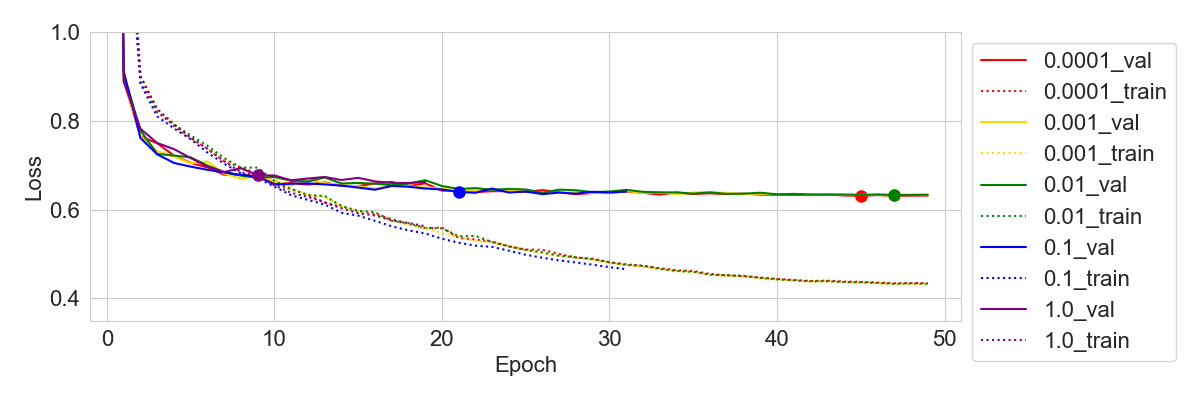
\includegraphics[height=55mm]{./figure/sec4/learning_curves/0/mel_loss.png}
        \caption{メルスペクトログラムについてのMAE Loss}
        \label{sec4:fig:learning_curve_baseline_val_mel_loss}
    \end{subfigure}
    \begin{subfigure}{\linewidth}
        \centering
        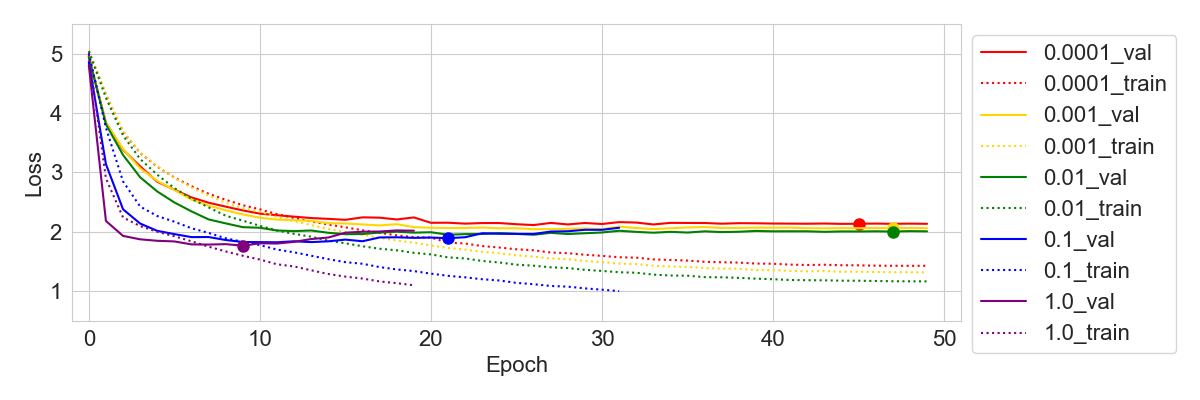
\includegraphics[height=55mm]{./figure/sec4/learning_curves/0/ssl_feature_cluster_loss.png}
        \caption{HuBERT離散特徴量についてのCross Entropy Loss}
        \label{sec4:fig:learning_curve_baseline_val_ssl_feature_cluster_loss}
    \end{subfigure}
    \begin{subfigure}{\linewidth}
        \centering
        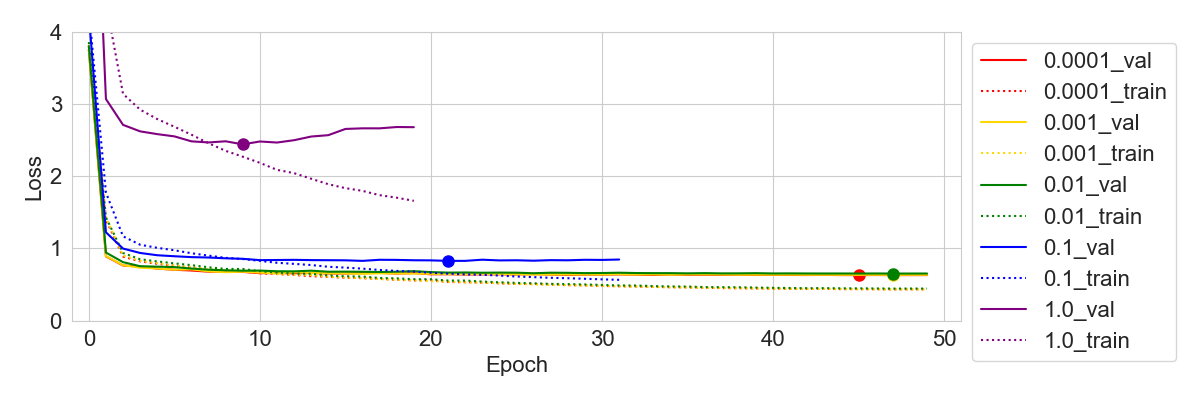
\includegraphics[height=55mm]{./figure/sec4/learning_curves/0/total_loss.png}
        \caption{損失の合計値}
        \label{sec4:fig:learning_curve_baseline_val_total_loss}
    \end{subfigure}
    \caption{ベースラインにおける学習曲線}
    \label{sec4:fig:learning_curve_baseline_val_losses}
\end{figure}

\begin{figure}[bt]
    \centering
    \begin{subfigure}{\linewidth}
        \centering
        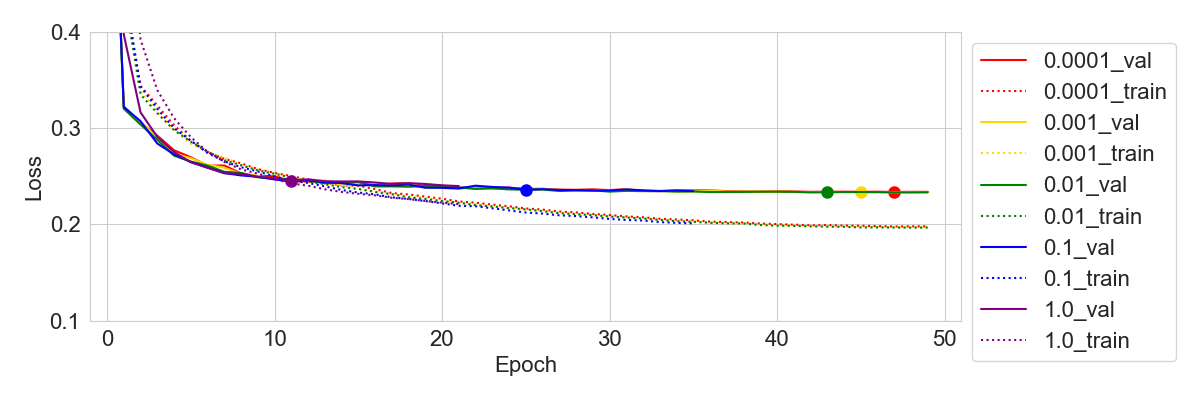
\includegraphics[height=45mm]{./figure/sec4/learning_curves/1/ssl_conv_feature_loss.png}
        \caption{HuBERT中間特徴量についてのMAE Loss}
        \label{sec4:fig:learning_curve_method_1_val_ssl_conv_feature_loss}
    \end{subfigure}
    \begin{subfigure}{\linewidth}
        \centering
        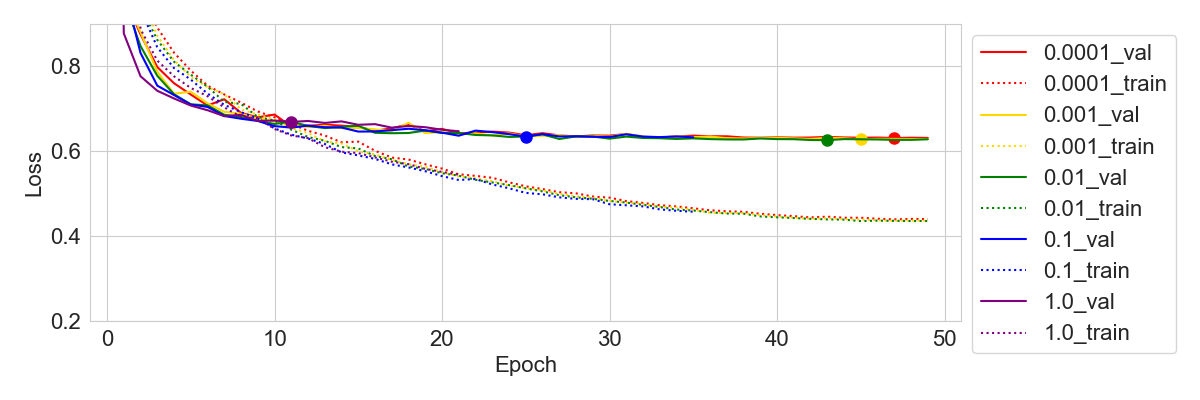
\includegraphics[height=45mm]{./figure/sec4/learning_curves/1/mel_loss.png}
        \caption{メルスペクトログラムについてのMAE Loss}
        \label{sec4:fig:learning_curve_method_1_val_mel_loss}
    \end{subfigure}
    \begin{subfigure}{\linewidth}
        \centering
        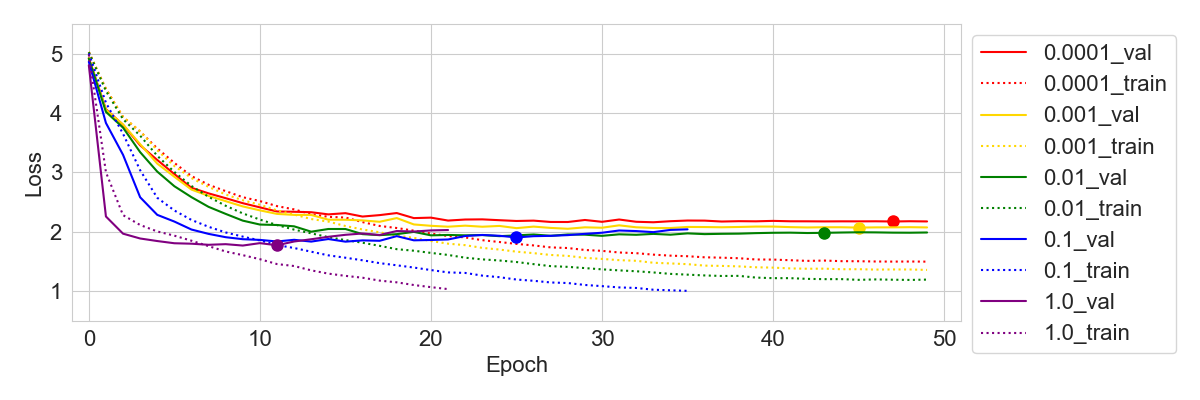
\includegraphics[height=45mm]{./figure/sec4/learning_curves/1/ssl_feature_cluster_loss.png}
        \caption{HuBERT離散特徴量についてのCross Entropy Loss}
        \label{sec4:fig:learning_curve_method_1_val_ssl_feature_cluster_loss}
    \end{subfigure}
    \begin{subfigure}{\linewidth}
        \centering
        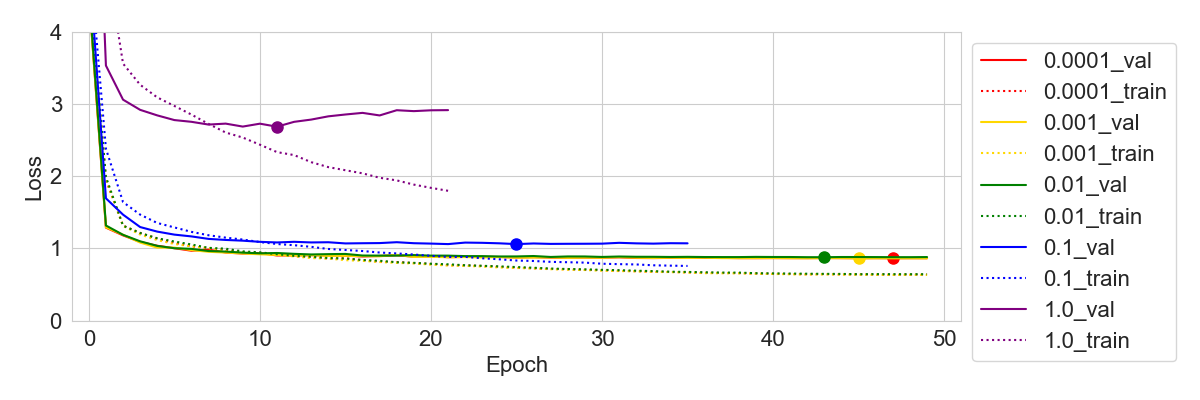
\includegraphics[height=45mm]{./figure/sec4/learning_curves/1/total_loss.png}
        \caption{損失の合計値}
        \label{sec4:fig:learning_curve_method_1_val_total_loss}
    \end{subfigure}
    \caption{ネットワークAにおける学習曲線}
    \label{sec4:fig:learning_curve_method_1_val_losses}
\end{figure}

\begin{figure}[bt]
    \centering
    \begin{subfigure}{\linewidth}
        \centering
        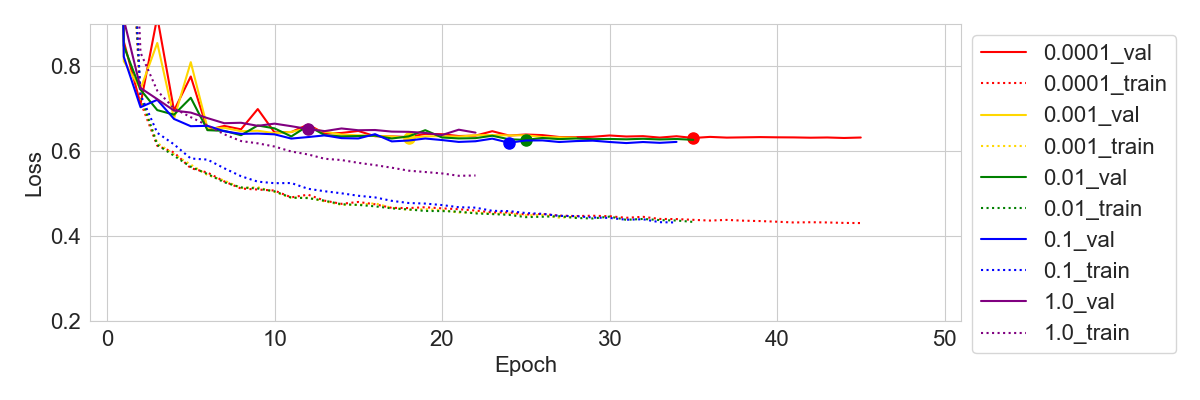
\includegraphics[height=55mm]{./figure/sec4/learning_curves/2/mel_loss.png}
        \caption{メルスペクトログラムについてのMAE Loss}
        \label{sec4:fig:learning_curve_method_2_val_mel_loss}
    \end{subfigure}
    \begin{subfigure}{\linewidth}
        \centering
        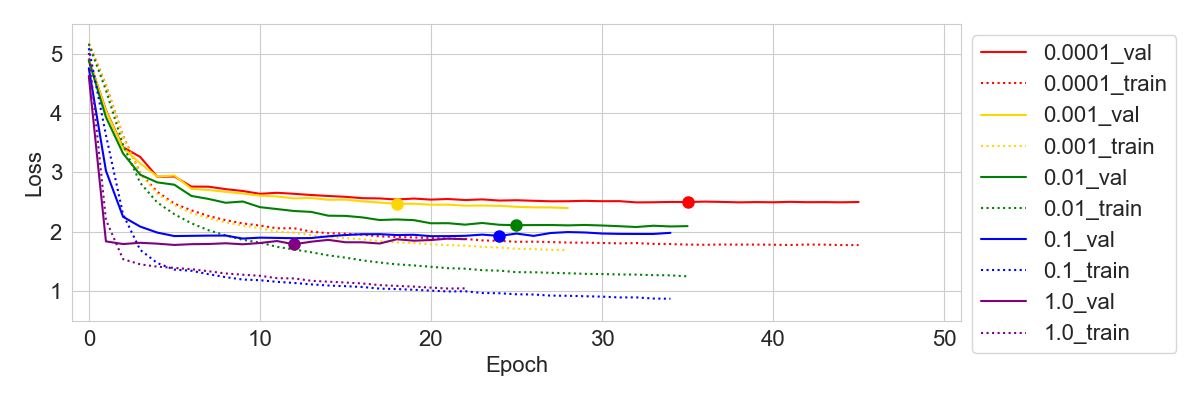
\includegraphics[height=55mm]{./figure/sec4/learning_curves/2/ssl_feature_cluster_loss.png}
        \caption{HuBERT離散特徴量についてのCross Entropy Loss}
        \label{sec4:fig:learning_curve_method_2_val_ssl_feature_cluster_loss}
    \end{subfigure}
    \begin{subfigure}{\linewidth}
        \centering
        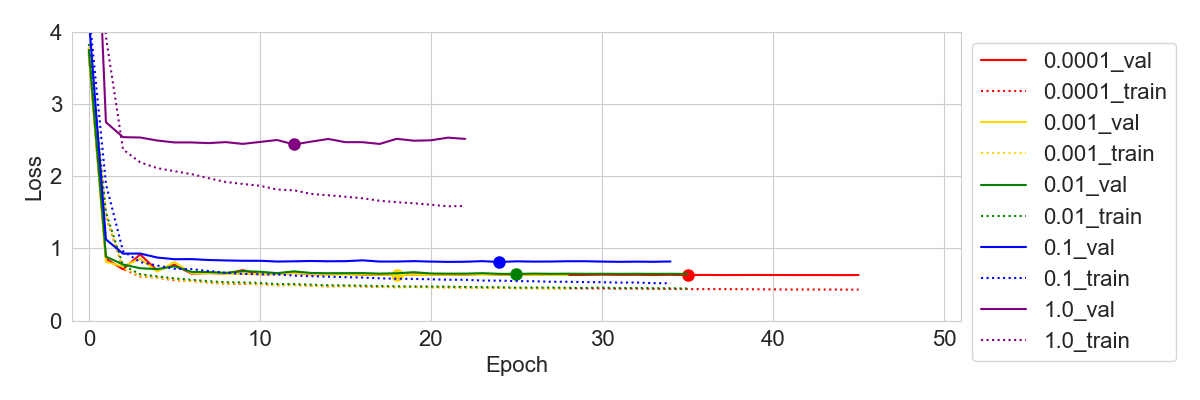
\includegraphics[height=55mm]{./figure/sec4/learning_curves/2/total_loss.png}
        \caption{損失の合計値}
        \label{sec4:fig:learning_curve_method_2_val_total_loss}
    \end{subfigure}
    \caption{ネットワークB(Randomized)における学習曲線}
    \label{sec4:fig:learning_curve_method_2_val_losses}
\end{figure}

\begin{figure}[bt]
    \centering
    \begin{subfigure}{\linewidth}
        \centering
        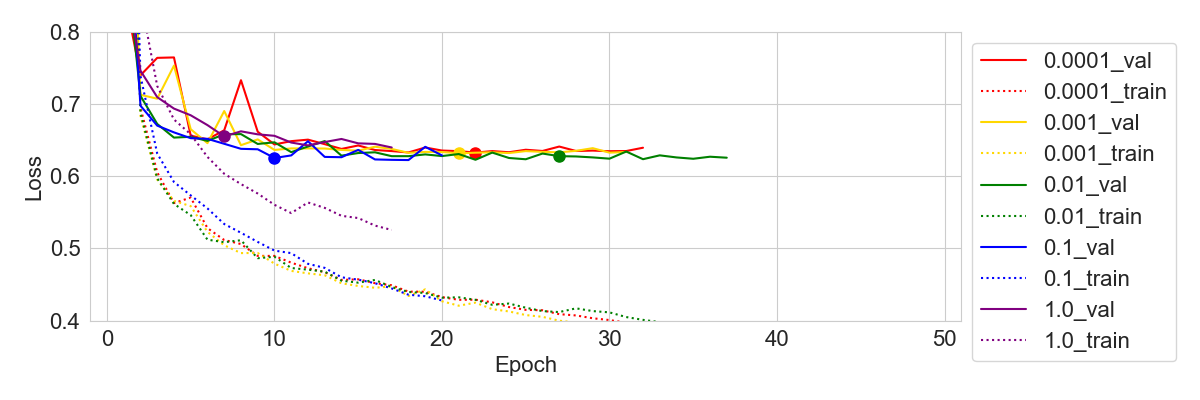
\includegraphics[height=55mm]{./figure/sec4/learning_curves/4/mel_loss.png}
        \caption{メルスペクトログラムについてのMAE Loss}
        \label{sec4:fig:learning_curve_method_4_val_mel_loss}
    \end{subfigure}
    \begin{subfigure}{\linewidth}
        \centering
        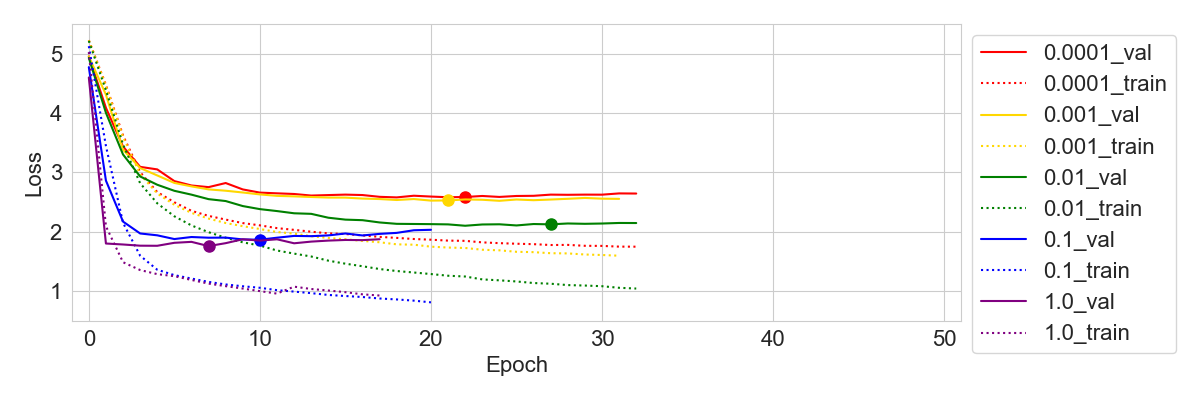
\includegraphics[height=55mm]{./figure/sec4/learning_curves/4/ssl_feature_cluster_loss.png}
        \caption{HuBERT離散特徴量についてのCross Entropy Loss}
        \label{sec4:fig:learning_curve_method_4_val_ssl_feature_cluster_loss}
    \end{subfigure}
    \begin{subfigure}{\linewidth}
        \centering
        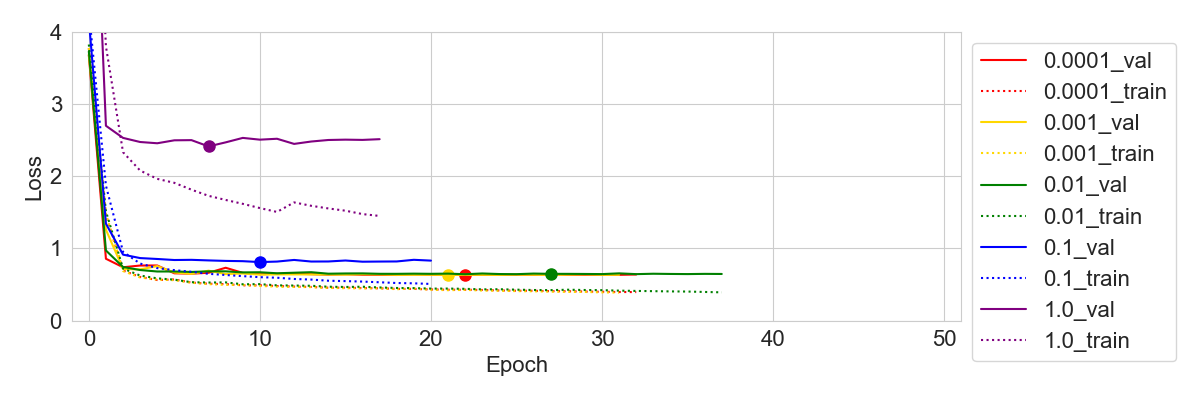
\includegraphics[height=55mm]{./figure/sec4/learning_curves/4/total_loss.png}
        \caption{損失の合計値}
        \label{sec4:fig:learning_curve_method_4_val_total_loss}
    \end{subfigure}
    \caption{ネットワークB(Pretrained)における学習曲線}
    \label{sec4:fig:learning_curve_method_4_val_losses}
\end{figure}

\begin{table}[bt]
    \centering
    \caption{最適な$\lossWeightHubDisc$における手法ごとの比較}
    \label{sec4:tab:obj_method_comp}
    \begin{center}
        \renewcommand{\arraystretch}{1.0} % 行の高さ調整
        \setlength{\tabcolsep}{8pt}      % 列の幅調整
        \scalebox{1.0}{
            \begin{tabular}{|c|l|rr|}
                \hline
                \multicolumn{1}{|c|}{手法} & \multicolumn{1}{c|}{$\lossWeightHubDisc$} & \multicolumn{1}{c}{WER [\%]} & \multicolumn{1}{c|}{話者類似度} \\
                \hline
                ベースライン                   & 0.001                                     & 54.6                         & 0.836                      \\
                ネットワークB(Randomized)      & 0.1                                       & 45.3                         & \underline{0.840}          \\
                ネットワークB(Pretrained)      & 0.1                                       & \underline{44.2}             & 0.778                      \\
                \hline
                分析合成                     & \multicolumn{1}{c|}{-}                    & 3.7                          & 0.956                      \\
                原音声                      & \multicolumn{1}{c|}{-}                    & 3.7                          & 1.000                      \\
                \hline
            \end{tabular}
        }
    \end{center}
\end{table}

\clearpage

\subsubsection{客観評価2: 提案手法のさらなる検討}
\label{sec4:sec:obj_2}
\ref{sec4:sec:obj_1}節において良好な結果を示したのはネットワークB(Randomized)であったが,これはHuBERTの転移学習による改善を狙った本実験の仮説に反する結果であった.これに対し,本節では良好な結果を示したネットワークB(Randomized)に焦点を当てたさらなる検討の結果を述べる.

まず,入力特徴量について検討した.\ref{sec4:sec:obj_1}節では事前学習済み重みを用いることの有効性を調べる目的があったため,入力特徴量はHuBERTの事前学習時に揃えて,HuBERT中間特徴量とした.しかし,ネットワークB(Randomized)は事前学習済み重みを利用しないため,HuBERT中間特徴量を入力とすることが意味をなしているか不明である.これに対し,ネットワークAからマルチタスク学習によって同時に予測される,メルスペクトログラムとHuBERT離散特徴量に対するロジットを組み合わせて入力する場合を比較した.メルスペクトログラムは,時間方向に隣接した2フレームを次元方向に積むことで160次元\SI{50}{\Hz}の特徴量に変換し,HuBERT離散特徴量に対するロジットは101次元\SI{50}{\Hz}の特徴量としてそのまま用いた.これらを次元方向に結合することで261次元\SI{50}{\Hz}の特徴量を構成し,全結合層を通してHuBERT中間特徴量と同じ768次元に変換することで,HuBERT Transformer層への入力とした.結果を表\ref{sec4:tab:obj_weights_networkb_input_comparison}に示す.新たに検討した手法はネットワークB(Randomized・Mel-HuB)とし,$\lossWeightHubDisc = 0.001$の場合が最適だと判断した.下線は掲載した手法全てにおける最良値を示す。これより,最適なネットワークB(Randomized・Mel-HuB)はネットワークB(Randomized)よりも話者類似度は0.005高いが,WERも10.1\%高いことが分かる.図\ref{sec4:fig:learning_curve_method_6_val_losses}にネットワークB(Randomized・Mel-HuB)の学習曲線を示す.傾向自体はネットワークB(Randomized)と概ね変わらないことがわかる。また,ネットワークB(Randomized)では$\lossWeightHubDisc$の値を大きくすることによって,0.0001から0.1までWERが低下傾向にあった.これに対し,ネットワークB(Randomized・Mel-HuB)ではWERの低下傾向は見られず,結果としてネットワークB(Randomized)に劣る結果となった.以上より,HuBERT中間特徴量は,メルスペクトログラムとHuBERT離散特徴量のロジットから構成した特徴量と比較して,ネットワークBの予測精度改善につながるより良い入力特徴量であったと考えられる.

\begin{table}[b]
    \centering
    \caption{HuBERT Transformer層への入力特徴量を変化させた場合の比較}
    \label{sec4:tab:obj_weights_networkb_input_comparison}
    \begin{center}
        \renewcommand{\arraystretch}{1.0} % 行の高さ調整
        \setlength{\tabcolsep}{8pt}      % 列の幅調整
        \scalebox{0.98}{
            \begin{tabular}{|c|l|rr|}
                \hline
                \multicolumn{1}{|c|}{手法}             & \multicolumn{1}{c|}{$\lossWeightHubDisc$} & \multicolumn{1}{c}{WER [\%]} & \multicolumn{1}{c|}{話者類似度} \\
                \hline
                ネットワークB(Randomized・Mel-HuB)          & 0.0001                                    & 59.5                         & 0.840                      \\
                \textbf{ネットワークB(Randomized・Mel-HuB)} & \textbf{0.001}                            & \textbf{55.4}                & \underline{\textbf{0.845}} \\
                ネットワークB(Randomized・Mel-HuB)          & 0.01                                      & 56.2                         & 0.803                      \\
                ネットワークB(Randomized・Mel-HuB)          & 0.1                                       & 57.7                         & 0.795                      \\
                ネットワークB(Randomized・Mel-HuB)          & 1                                         & 58.1                         & 0.711                      \\
                \hline
                ネットワークB(Randomized)                  & 0.1                                       & \underline{45.3}             & 0.840                      \\
                \hline
            \end{tabular}
        }
    \end{center}
\end{table}

\begin{figure}[bt]
    \centering
    \begin{subfigure}{\linewidth}
        \centering
        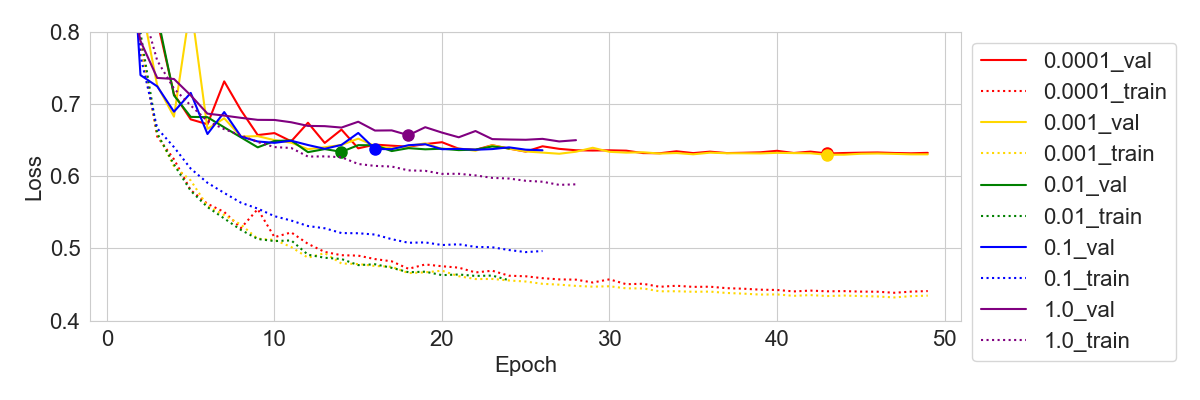
\includegraphics[height=55mm]{./figure/sec4/learning_curves/6/mel_loss.png}
        \caption{メルスペクトログラムについてのMAE Loss}
        \label{sec4:fig:learning_curve_method_6_val_mel_loss}
    \end{subfigure}
    \begin{subfigure}{\linewidth}
        \centering
        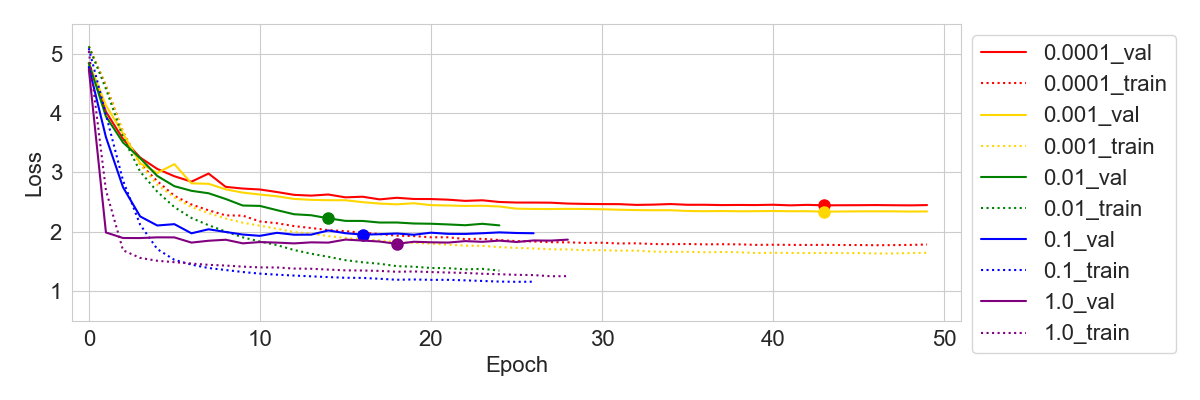
\includegraphics[height=55mm]{./figure/sec4/learning_curves/6/ssl_feature_cluster_loss.png}
        \caption{HuBERT離散特徴量についてのCross Entropy Loss}
        \label{sec4:fig:learning_curve_method_6_val_ssl_feature_cluster_loss}
    \end{subfigure}
    \begin{subfigure}{\linewidth}
        \centering
        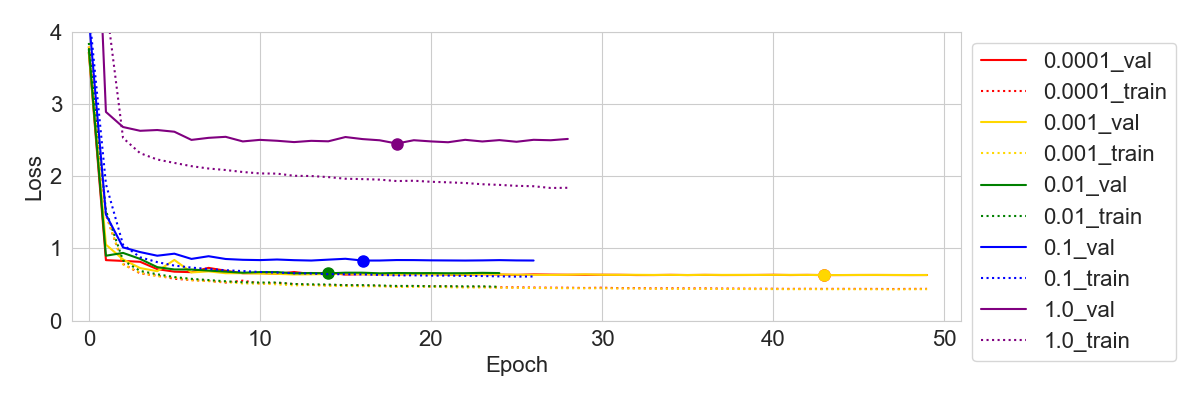
\includegraphics[height=55mm]{./figure/sec4/learning_curves/6/total_loss.png}
        \caption{損失の合計値}
        \label{sec4:fig:learning_curve_method_6_val_total_loss}
    \end{subfigure}
    \caption{ネットワークB(Randomized・Mel-HuB)における学習曲線}
    \label{sec4:fig:learning_curve_method_6_val_losses}
\end{figure}

次に,HuBERT中間特徴量をネットワークBに与えている,ネットワークAの学習方法を検討した.ここでは,これまでネットワークAで採用していたHuBERT中間特徴量,メルスペクトログラム,HuBERT離散特徴量を予測するマルチタスク学習に対し,HuBERT中間特徴量のみを予測するシングルタスク学習の場合を比較した.結果を表\ref{sec4:tab:obj_weights_networka_multitask}に示す.新たに検討した手法はネットワークB(Randomized・A-SingleTask)とし,$\lossWeightHubDisc = 0.1$の場合が最適だと判断した.これより,最適なネットワークB(Randomized・A-SingleTask)はネットワークB(Randomized)よりもWERが2.8\%低く,話者類似度は0.007高いことがわかる.図\ref{sec4:fig:learning_curve_method_9_val_losses}にネットワークB(Randomized・A-SingleTask)の学習曲線を示す.これはネットワークB(Randomized)と概ね同様の傾向であった.以上より,ネットワークAではHuBERT中間特徴量,メルスペクトログラム,HuBERT離散特徴量を予測するマルチタスク学習行うよりも,HuBERT中間特徴量のみを予測する方が,ネットワークBに対してより良い入力特徴量を与えられるのだと考えられる.

\begin{table}[bt]
    \centering
    \caption{ネットワークAにおけるマルチタスク学習の有無による比較}
    \label{sec4:tab:obj_weights_networka_multitask}
    \begin{center}
        \renewcommand{\arraystretch}{1.0} % 行の高さ調整
        \setlength{\tabcolsep}{8pt}      % 列の幅調整
        \scalebox{0.99}{
            \begin{tabular}{|c|l|rr|}
                \hline
                \multicolumn{1}{|c|}{手法}                  & \multicolumn{1}{c|}{$\lossWeightHubDisc$} & \multicolumn{1}{c}{WER [\%]} & \multicolumn{1}{c|}{話者類似度} \\
                \hline
                ネットワークB(Randomized・A-SingleTask)          & 0.0001                                    & 54.0                         & \underline{0.867}          \\
                ネットワークB(Randomized・A-SingleTask)          & 0.001                                     & 52.2                         & 0.865                      \\
                ネットワークB(Randomized・A-SingleTask)          & 0.01                                      & 51.8                         & 0.843                      \\
                \textbf{ネットワークB(Randomized・A-SingleTask)} & \textbf{0.1}                              & \underline{\textbf{42.5}}    & \textbf{0.847}             \\
                ネットワークB(Randomized・A-SingleTask)          & 1                                         & 43.0                         & 0.768                      \\
                \hline
                ネットワークB(Randomized)                       & 0.1                                       & 45.3                         & 0.840                      \\
                \hline
            \end{tabular}
        }
    \end{center}
\end{table}

\begin{figure}[bt]
    \centering
    \begin{subfigure}{\linewidth}
        \centering
        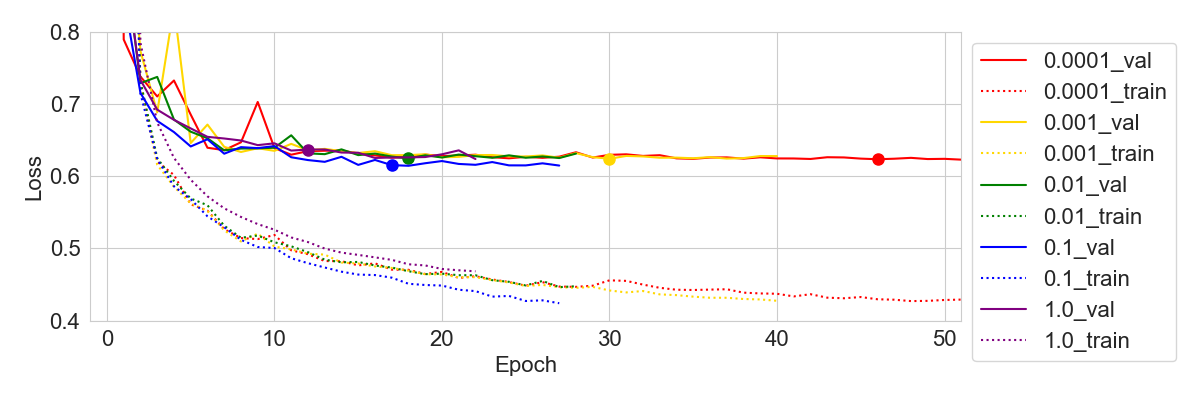
\includegraphics[height=55mm]{./figure/sec4/learning_curves/9/mel_loss.png}
        \caption{メルスペクトログラムについてのMAE Loss}
        \label{sec4:fig:learning_curve_method_9_val_mel_loss}
    \end{subfigure}
    \begin{subfigure}{\linewidth}
        \centering
        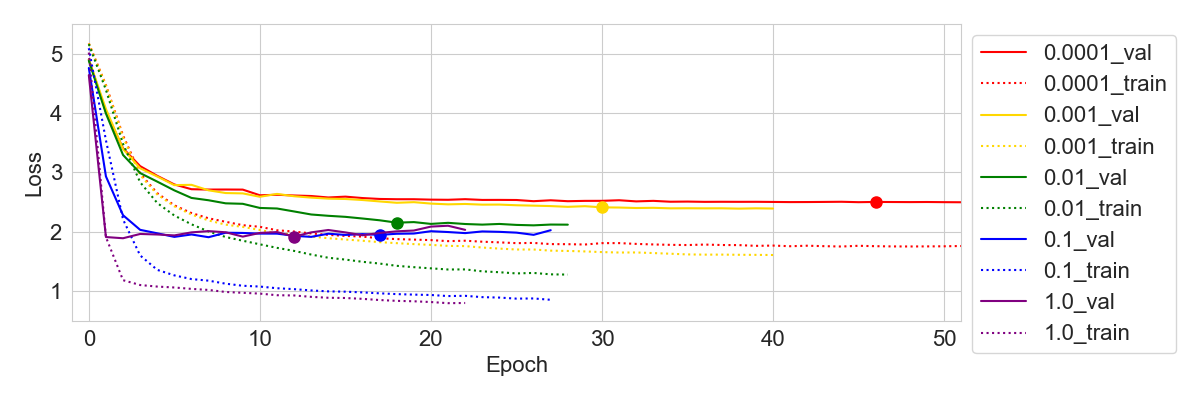
\includegraphics[height=55mm]{./figure/sec4/learning_curves/9/ssl_feature_cluster_loss.png}
        \caption{HuBERT離散特徴量についてのCross Entropy Loss}
        \label{sec4:fig:learning_curve_method_9_val_ssl_feature_cluster_loss}
    \end{subfigure}
    \begin{subfigure}{\linewidth}
        \centering
        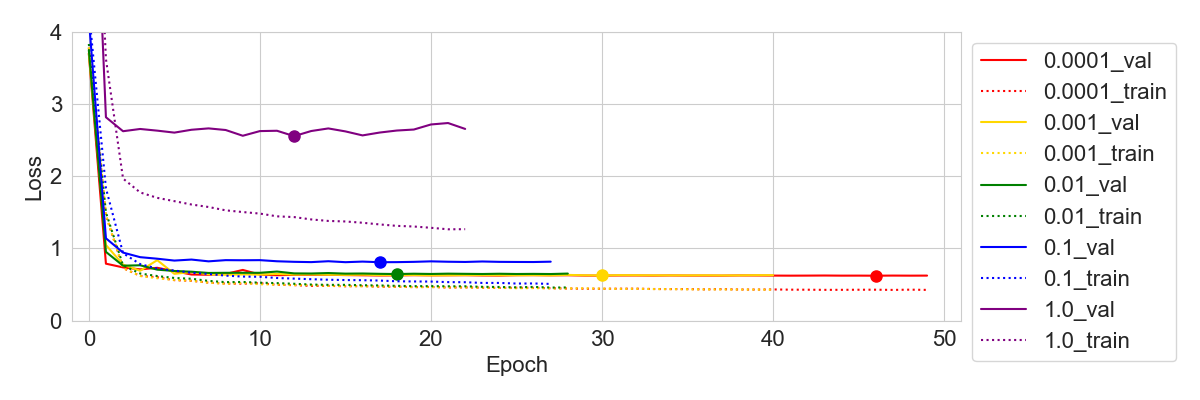
\includegraphics[height=55mm]{./figure/sec4/learning_curves/9/total_loss.png}
        \caption{損失の合計値}
        \label{sec4:fig:learning_curve_method_9_val_total_loss}
    \end{subfigure}
    \caption{ネットワークB(Randomized・A-SingleTask)における学習曲線}
    \label{sec4:fig:learning_curve_method_9_val_losses}
\end{figure}

最後に,これまでネットワークAとネットワークBを2段階で学習させたのに対し,ネットワークAからネットワークBまでを一度に学習させる方法を検討した.これにより,HuBERT中間特徴量に表現力を制限させないことで,さらなる精度改善を狙った.ここでは,ネットワークBの出力に対する損失関数$\lossB$のみを用いて学習させ,ネットワークAの出力は単にネットワークBへの入力とした.ネットワークAおよびネットワークB(Randomized)を未学習の状態で初期化した場合の結果を表\ref{sec4:tab:obj_weights_e2e_randomized}に示す.新たに検討した手法はネットワークE2E(Randomized)とし,$\lossWeightHubDisc = 0.1$が最適だと判断した.これより,最適なネットワークE2E(Randomized)はネットワークB(Randomized・A-SingleTask)よりもWERが20.0\%高く,話者類似度は0.080低いことがわかる.図\ref{sec4:fig:learning_curve_method_7_val_losses}に学習曲線を示す.2段階で学習させたネットワークB(Randomized・A-SingleTask)と比較して損失の下がりが悪く,客観評価指標が顕著に悪化したことは妥当だと考える.以上より,2段階学習は学習の安定化につながっていたと言える.次に,ここまでの検討で最も良好な結果を示した,ネットワークB(Randomized・A-SingleTask)かつ$\lossWeightHubDisc = 0.1$の場合における学習済み重みでネットワークAとネットワークBを初期化した場合の結果を表\ref{sec4:tab:obj_weights_e2e_pretrained}に示す.新たに検討した手法はネットワークE2E(Pretrained)とし,ここでは$\lossWeightHubDisc$の値は0.1のままで固定して,スケジューラであるCosine Annealing with Warmupの最大学習率$\learningRate_{\text{max}}$を変更することでチューニングした.最適値は$\learningRate_{\text{max}} = 5.0 \times 10^{-5}$とした.これより,最適なネットワークE2E(Pretrained)はネットワークB(Randomized・A-SingleTask)よりもWERが1.3\%高く,話者類似度も0.006高いことがわかる.図\ref{sec4:fig:learning_curve_method_10_11_12_val_losses}に学習曲線を示す.線の色は$\learningRate_{\text{max}}$の違いを表す.損失が学習開始時からほとんど低下していないため,ネットワーク全体を再学習することは効果的でなかったと考えられる.

\begin{table}[bt]
    \centering
    \caption{ネットワークAからネットワークBまでを未学習の状態で初期化し,一度に学習させた場合の比較}
    \label{sec4:tab:obj_weights_e2e_randomized}
    \begin{center}
        \renewcommand{\arraystretch}{1.0} % 行の高さ調整
        \setlength{\tabcolsep}{8pt}      % 列の幅調整
        \scalebox{1.0}{
            \begin{tabular}{|c|l|rr|}
                \hline
                \multicolumn{1}{|c|}{手法}         & \multicolumn{1}{c|}{$\lossWeightHubDisc$} & \multicolumn{1}{c}{WER [\%]} & \multicolumn{1}{c|}{話者類似度} \\
                \hline
                ネットワークE2E(Randomized)            & 0.0001                                    & 101.0                        & 0.543                      \\
                ネットワークE2E(Randomized)            & 0.001                                     & 121.9                        & 0.551                      \\
                ネットワークE2E(Randomized)            & 0.01                                      & 101.1                        & 0.507                      \\
                \textbf{ネットワークE2E(Randomized)}   & \textbf{0.1}                              & \textbf{62.0}                & \textbf{0.767}             \\
                ネットワークE2E(Randomized)            & 1                                         & 71.1                         & 0.643                      \\
                \hline
                ネットワークB(Randomized・A-SingleTask) & 0.1                                       & \underline{42.5}             & \underline{0.847}          \\
                \hline
            \end{tabular}
        }
    \end{center}
\end{table}

\begin{figure}[bt]
    \centering
    \begin{subfigure}{\linewidth}
        \centering
        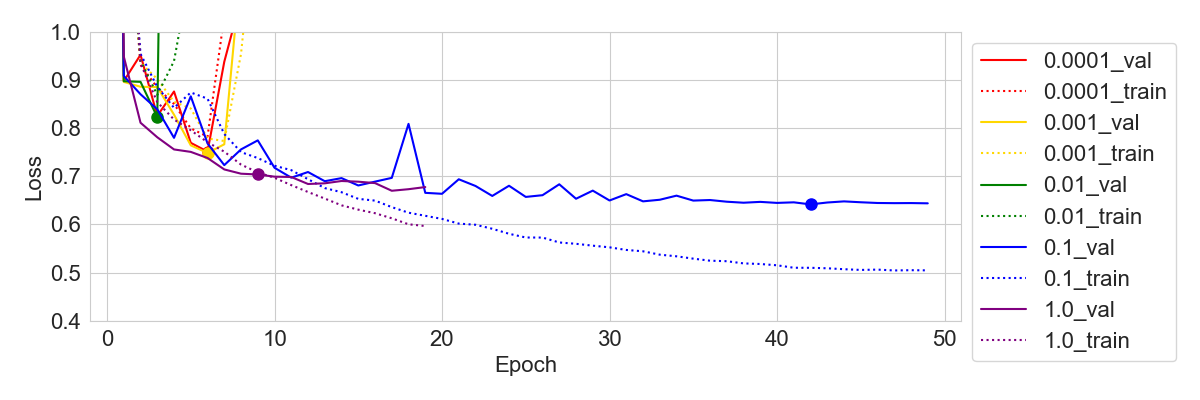
\includegraphics[height=55mm]{./figure/sec4/learning_curves/7/mel_loss.png}
        \caption{メルスペクトログラムについてのMAE Loss}
        \label{sec4:fig:learning_curve_method_7_val_mel_loss}
    \end{subfigure}
    \begin{subfigure}{\linewidth}
        \centering
        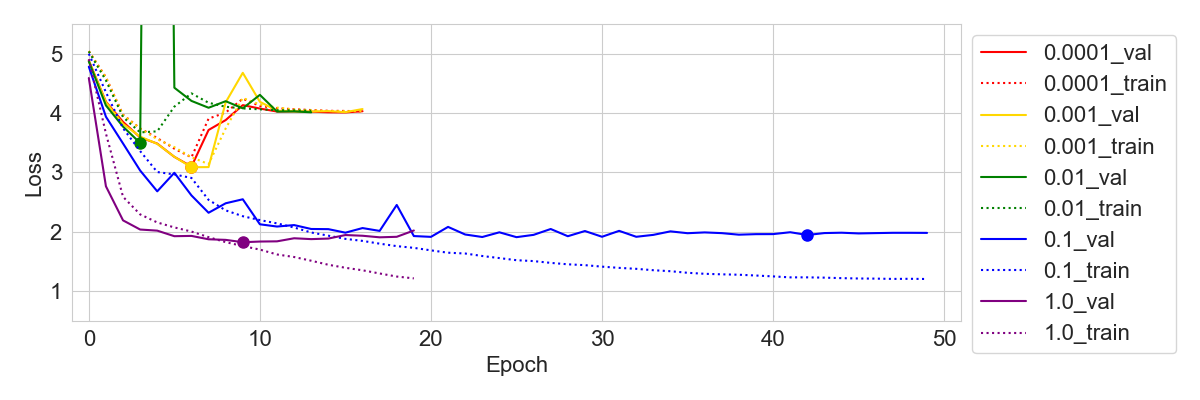
\includegraphics[height=55mm]{./figure/sec4/learning_curves/7/ssl_feature_cluster_loss.png}
        \caption{HuBERT離散特徴量についてのCross Entropy Loss}
        \label{sec4:fig:learning_curve_method_7_val_ssl_feature_cluster_loss}
    \end{subfigure}
    \begin{subfigure}{\linewidth}
        \centering
        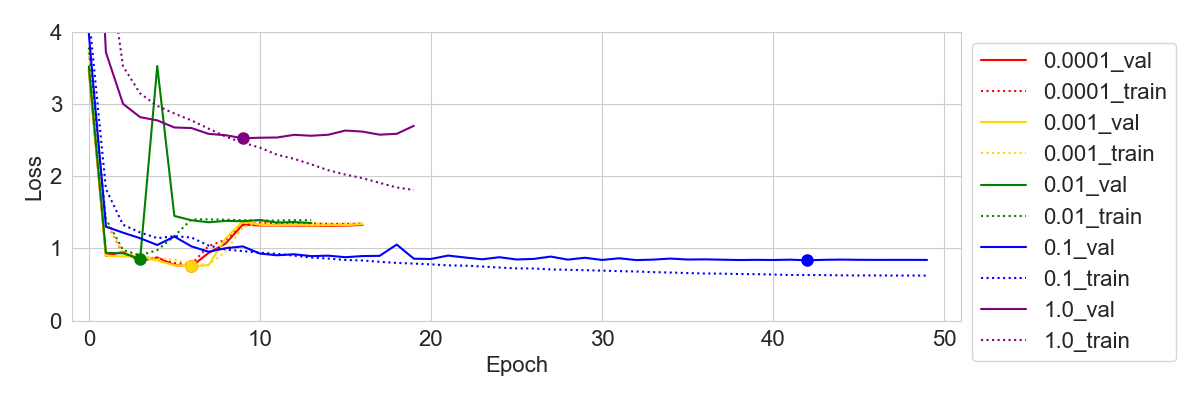
\includegraphics[height=55mm]{./figure/sec4/learning_curves/7/total_loss.png}
        \caption{損失の合計値}
        \label{sec4:fig:learning_curve_method_7_val_total_loss}
    \end{subfigure}
    \caption{ネットワークE2E(Randomized)における学習曲線}
    \label{sec4:fig:learning_curve_method_7_val_losses}
\end{figure}

\begin{table}[bt]
    \centering
    \caption{ネットワークB(Randomized・A-SingleTask)かつ$\lossWeightHubDisc = 0.1$の場合における学習済み重みでネットワークAとネットワークBを初期化し,一度に学習させた場合の比較}
    \label{sec4:tab:obj_weights_e2e_pretrained}
    \begin{center}
        \renewcommand{\arraystretch}{1.0} % 行の高さ調整
        \setlength{\tabcolsep}{8pt}      % 列の幅調整
        \scalebox{1.0}{
            \begin{tabular}{|c|l|rr|}
                \hline
                \multicolumn{1}{|c|}{手法}         & \multicolumn{1}{c|}{$\learningRate_{\text{max}}$} & \multicolumn{1}{c}{WER [\%]} & \multicolumn{1}{c|}{話者類似度} \\
                \hline
                ネットワークE2E(Pretrained)            & $5.0 \times 10^{-4}$                              & 44.6                         & 0.851                      \\
                \textbf{ネットワークE2E(Pretrained)}   & $\mathbf{5.0 \times 10^{-5}}$                     & \textbf{43.5}                & \underline{\textbf{0.853}} \\
                ネットワークE2E(Pretrained)            & $5.0 \times 10^{-6}$                              & 43.6                         & \underline{0.853}          \\
                \hline
                ネットワークB(Randomized・A-SingleTask) & $5.0 \times 10^{-4}$                              & \underline{42.5}             & 0.847                      \\
                \hline
            \end{tabular}
        }
    \end{center}
\end{table}

\begin{figure}[bt]
    \centering
    \begin{subfigure}{\linewidth}
        \centering
        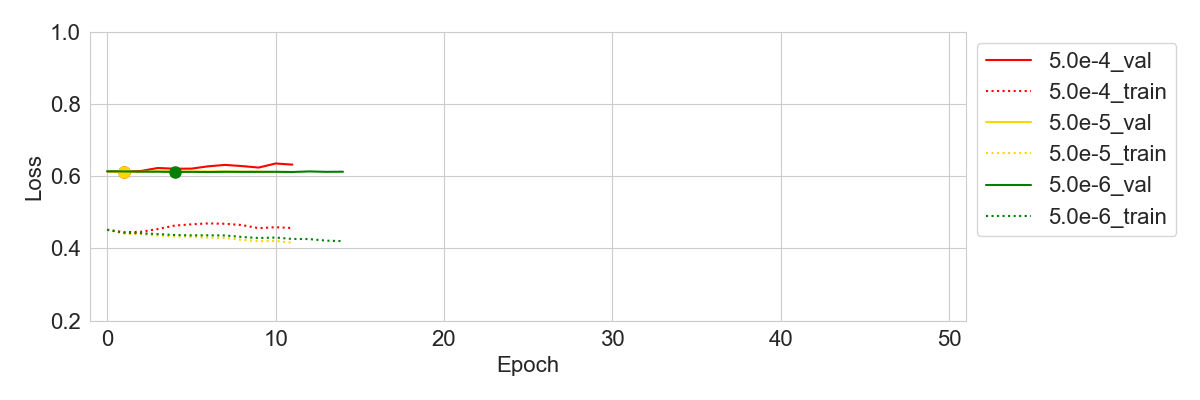
\includegraphics[height=55mm]{./figure/sec4/learning_curves/10_11_12/mel_loss.png}
        \caption{メルスペクトログラムについてのMAE Loss}
        \label{sec4:fig:learning_curve_method_10_11_12_val_mel_loss}
    \end{subfigure}
    \begin{subfigure}{\linewidth}
        \centering
        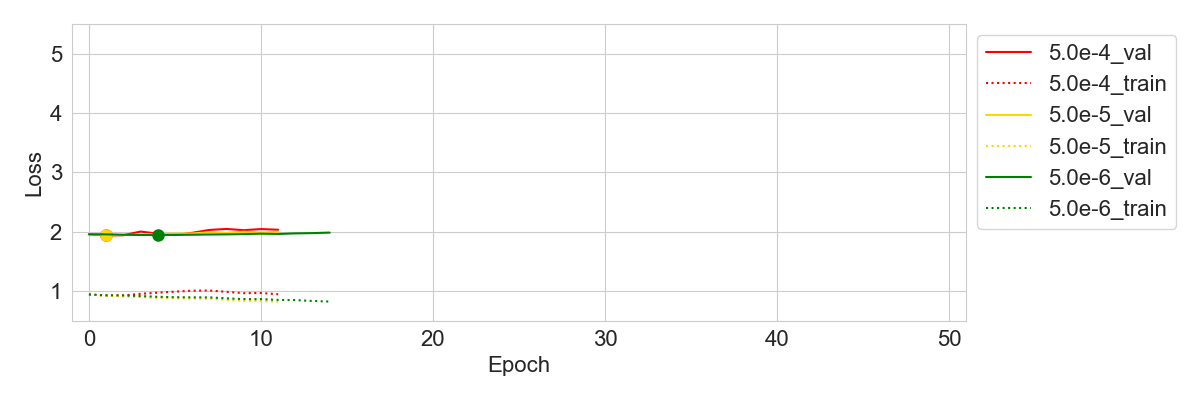
\includegraphics[height=55mm]{./figure/sec4/learning_curves/10_11_12/ssl_feature_cluster_loss.png}
        \caption{HuBERT離散特徴量についてのCross Entropy Loss}
        \label{sec4:fig:learning_curve_method_10_11_12_val_ssl_feature_cluster_loss}
    \end{subfigure}
    \begin{subfigure}{\linewidth}
        \centering
        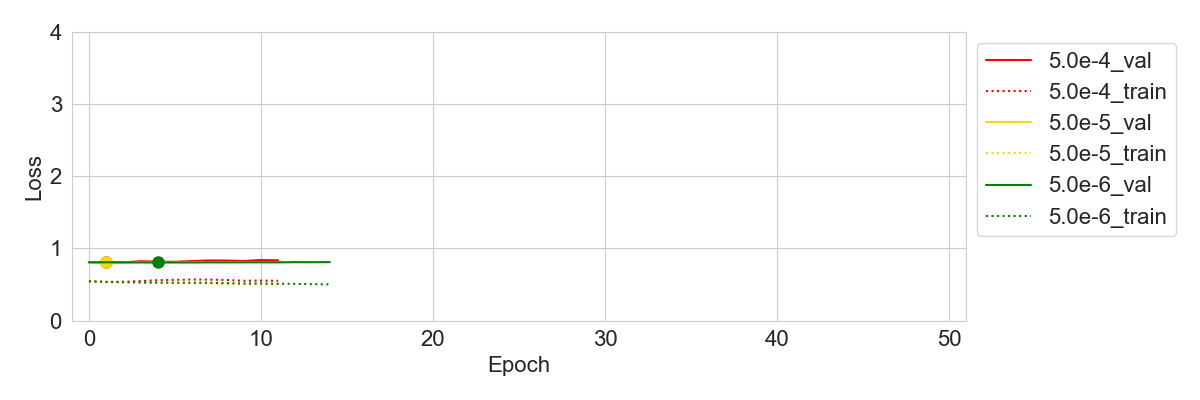
\includegraphics[height=55mm]{./figure/sec4/learning_curves/10_11_12/total_loss.png}
        \caption{損失の合計値}
        \label{sec4:fig:learning_curve_method_10_11_12_val_total_loss}
    \end{subfigure}
    \caption{ネットワークE2E(Pretrained)における学習曲線}
    \label{sec4:fig:learning_curve_method_10_11_12_val_losses}
\end{figure}

\clearpage

\subsubsection{主観評価}
主観評価実験では,\ref{sec4:sec:obj_1}節および\ref{sec4:sec:obj_2}節の検討結果を踏まえ,以下の5種類の音声を評価対象とした.
\begin{enumerate}
    \item ベースライン
    \item ネットワークB(Randomized)
    \item ネットワークB(Randomized・A-SingleTask)
    \item 分析合成
    \item 原音声
\end{enumerate}
ここで,ネットワークB(Randomized)およびネットワークB(Randomized・A-SingleTask)が,今回の実験を通して選択した提案手法の代表である.\ref{sec4:sec:sbj_explanation}節で述べたように,主観評価では音声の明瞭性と類似性の5段階評価を実施した.ダミー音声に対する評価値を誤った被験者は存在しなかったため,75人分のデータを統計処理に用いた.

被験者に対するアンケート結果について述べる.年齢層は21歳から62歳に渡り,箱ひげ図にてその分布を示した(図\ref{sec4:fig:age}).性別の内訳は男性32名,女性43名であり,実験に利用した音響機器の内訳はヘッドホンが19名,イヤホンが56名であった.
\begin{figure}[b]
    \centering
    \includegraphics[height=50mm]{./figure/sec4/sbj/age.png}
    \caption{主観評価実験における被験者の年齢層}
    \label{sec4:fig:age}
\end{figure}

明瞭性と類似性の評価値について,手法ごとの標本平均と95\%信頼区間を表\ref{sec4:tab:sbj_mean_ci}に示す.また,各手法の組み合わせについて,平均値の差の検定(Welchのt検定)を行った結果を表\ref{sec4:tab:sbj_int_p}, \ref{sec4:tab:sbj_sim_p}に示す.表における$\lr{i, j}$成分は,$i$行目の手法に対する評価値の母平均を$\mu_{i}$,$j$列目の手法に対する評価値の母平均を$\mu_{j}$とするとき,帰無仮説を$\mu_{i} = \mu_{j}$,対立仮説を$\mu_{i} > \mu_{j}$と片側検定で計算されたp値に対し,Benjamini/Hochberg法による多重比較のための補正を行った結果である.ここで,表の文字列は以下の意味である.
\begin{enumerate}
    \item GT: 原音声(Ground Truth)
    \item AbS: 分析合成(Analysis by Synthesis)
    \item B(Rand, A-S): ネットワークB(Randomized・A-SingleTask)
    \item B(Rand): ネットワークB(Randomized)
    \item Baseline: ベースライン
\end{enumerate}
また,本実験における有意水準は5\%とした.

まず,表\ref{sec4:tab:sbj_int_p}より,提案したネットワークB(Randomized)およびネットワークB(Randomized・A-SingleTask)は,ベースラインよりも明瞭性の評価値が有意に高いことがわかる.一方,ネットワークB(Randomized)とネットワークB(Randomized・A-SingleTask)の間に有意差がないことから,ネットワークAの学習方法の違いは明瞭性に顕著な違いをもたらさなかったと考えられる.次に,表\ref{sec4:tab:sbj_sim_p}より,提案したネットワークB(Randomized)およびネットワークB(Randomized・A-SingleTask)は,ベースラインよりも類似性の評価値が有意に高いことがわかる.また,ここではネットワークB(Randomized・A-SingleTask)がネットワークB(Randomized)よりも類似性の評価値が有意に高いこともわかる.従って,明瞭性と類似性の評価結果を合わせると,ネットワークB(Randomized・A-SingleTask)が最も優れた動画音声合成モデルであったと考えられる.

また,良好な結果を示したネットワークB(Randomized・A-SingleTask)であっても、分析合成や原音声との間には依然として大きな差があることがわかる。これより,本研究の目的であったベースラインからの改善は達成されたものの,原音声に匹敵する合成音声には至っていないと言える.従って,今後さらなるネットワークの改善が必要だと考える.

\begin{table}[bt]
    \centering
    \caption{主観評価実験の結果より計算した標本平均と95\%信頼区間}
    \label{sec4:tab:sbj_mean_ci}
    \begin{center}
        \renewcommand{\arraystretch}{1.0} % 行の高さ調整
        \setlength{\tabcolsep}{8pt}      % 列の幅調整
        \scalebox{0.95}{
            \begin{tabular}{|c|l|rr|}
                \hline
                \multicolumn{1}{|c|}{手法}         & \multicolumn{1}{c|}{$\lossWeightHubDisc$} & \multicolumn{1}{c}{明瞭性} & \multicolumn{1}{c|}{類似性} \\
                \hline
                ベースライン                           & 0.001                                     & $2.37 \pm 0.07$         & $2.92 \pm 0.08$          \\
                ネットワークB(Randomized)              & 0.1                                       & $2.76 \pm 0.07$         & $3.04 \pm 0.08$          \\
                ネットワークB(Randomized・A-SingleTask) & 0.1                                       & $2.82 \pm 0.08$         & $3.18 \pm 0.08$          \\
                \hline
                分析合成                             & \multicolumn{1}{c|}{-}                    & $4.75 \pm 0.04$         & $4.31 \pm 0.07$          \\
                原音声                              & \multicolumn{1}{c|}{-}                    & $4.87 \pm 0.03$         & $4.71 \pm 0.05$          \\
                \hline
            \end{tabular}
        }
    \end{center}
\end{table}

\begin{table}[bt]
    \centering
    \caption{主観評価実験の結果より計算した平均値の差の検定におけるp値(明瞭性)}
    \label{sec4:tab:sbj_int_p}
    \begin{center}
        \renewcommand{\arraystretch}{1.0} % 行の高さ調整
        \setlength{\tabcolsep}{8pt}      % 列の幅調整
        \scalebox{0.95}{
            \begin{tabular}{|c|rrrr|}
                \hline
                \multicolumn{1}{|c|}{} & \multicolumn{1}{c}{AbS} & \multicolumn{1}{c}{B(Rand, A-S)} & \multicolumn{1}{c}{B(Rand)} & \multicolumn{1}{c|}{Baseline} \\
                \hline
                GT                     & $6.67 \times 10^{-6}$   & $6.17 \times 10^{-262}$          & $2.84 \times 10^{-289}$     & $0$                           \\
                AbS                    & \multicolumn{1}{c}{-}   & $3.22 \times 10^{-243}$          & $2.40 \times 10^{-270}$     & $0$                           \\
                B(Rand, A-S)           & \multicolumn{1}{c}{-}   & \multicolumn{1}{c}{-}            & $1.23 \times 10^{-1}$       & $7.07 \times 10^{-17}$        \\
                B(Rand)                & \multicolumn{1}{c}{-}   & \multicolumn{1}{c}{-}            & \multicolumn{1}{c}{-}       & $1.12 \times 10^{-13}$        \\
                \hline
            \end{tabular}
        }
    \end{center}
\end{table}

\begin{table}[bt]
    \centering
    \caption{主観評価実験の結果より計算した平均値の差の検定におけるp値(類似性)}
    \label{sec4:tab:sbj_sim_p}
    \begin{center}
        \renewcommand{\arraystretch}{1.0} % 行の高さ調整
        \setlength{\tabcolsep}{8pt}      % 列の幅調整
        \scalebox{0.95}{
            \begin{tabular}{|c|rrrr|}
                \hline
                \multicolumn{1}{|c|}{} & \multicolumn{1}{c}{AbS} & \multicolumn{1}{c}{B(Rand, A-S)} & \multicolumn{1}{c}{B(Rand)} & \multicolumn{1}{c|}{Baseline} \\
                \hline
                GT                     & $1.24 \times 10^{-18}$  & $5.86 \times 10^{-160}$          & $9.90 \times 10^{-174}$     & $1.28 \times 10^{-205}$       \\
                AbS                    & \multicolumn{1}{c}{-}   & $3.11 \times 10^{-83}$           & $1.73 \times 10^{-97}$      & $3.58 \times 10^{-120}$       \\
                B(Rand, A-S)           & \multicolumn{1}{c}{-}   & \multicolumn{1}{c}{-}            & $1.13 \times 10^{-2}$       & $5.46 \times 10^{-6}$         \\
                B(Rand)                & \multicolumn{1}{c}{-}   & \multicolumn{1}{c}{-}            & \multicolumn{1}{c}{-}       & $2.13 \times 10^{-2}$         \\
                \hline
            \end{tabular}
        }
    \end{center}
\end{table}
\subsection{考察}

\clearpage

\section{結論}

\clearpage

\section*{謝辞}
\addcontentsline{toc}{section}{謝辞}
本研究に取り組む上で熱心に指導してくださり,計算環境やクラウドワークスなど,研究を進める上で必要となった新しい取り組みにも前向きに協力してくださった鏑木先生に,深く感謝申し上げます.

また,たくさん声をかけてくださり,研究を含め多く相談に乗っていただいた藤田さんをはじめ,ゼミなどで様々な意見をくださった研究室の方々,中間発表において意見をくださった河原先生,吉永先生に,深く感謝申し上げます.

\clearpage

\bibliographystyle{junsrt}
\addcontentsline{toc}{section}{参考文献}
\bibliography{library}

\end{document}